% Latex header for doxygen 1.8.4
\documentclass[twoside]{book}

% Packages required by doxygen
\usepackage{calc}
\usepackage{doxygen}
\usepackage{graphicx}
\usepackage[utf8]{inputenc}
\usepackage{makeidx}
\usepackage{multicol}
\usepackage{multirow}
\usepackage{textcomp}
\usepackage[table]{xcolor}

% Font selection
\usepackage[T1]{fontenc}
\usepackage{mathptmx}
\usepackage[scaled=.90]{helvet}
\usepackage{courier}
\usepackage{amssymb}
\usepackage{sectsty}
\renewcommand{\familydefault}{\sfdefault}
\allsectionsfont{%
  \fontseries{bc}\selectfont%
  \color{darkgray}%
}
\renewcommand{\DoxyLabelFont}{%
  \fontseries{bc}\selectfont%
  \color{darkgray}%
}

% Page & text layout
\usepackage{geometry}
\geometry{%
  a4paper,%
  top=2.5cm,%
  bottom=2.5cm,%
  left=2.5cm,%
  right=2.5cm%
}
\tolerance=750
\hfuzz=15pt
\hbadness=750
\setlength{\emergencystretch}{15pt}
\setlength{\parindent}{0cm}
\setlength{\parskip}{0.2cm}
\makeatletter
\renewcommand{\paragraph}{%
  \@startsection{paragraph}{4}{0ex}{-1.0ex}{1.0ex}{%
    \normalfont\normalsize\bfseries\SS@parafont%
  }%
}
\renewcommand{\subparagraph}{%
  \@startsection{subparagraph}{5}{0ex}{-1.0ex}{1.0ex}{%
    \normalfont\normalsize\bfseries\SS@subparafont%
  }%
}
\makeatother

% Headers & footers
\usepackage{fancyhdr}
\pagestyle{fancyplain}
\fancyhead[LE]{\fancyplain{}{\bfseries\thepage}}
\fancyhead[CE]{\fancyplain{}{}}
\fancyhead[RE]{\fancyplain{}{\bfseries\leftmark}}
\fancyhead[LO]{\fancyplain{}{\bfseries\rightmark}}
\fancyhead[CO]{\fancyplain{}{}}
\fancyhead[RO]{\fancyplain{}{\bfseries\thepage}}
\fancyfoot[LE]{\fancyplain{}{}}
\fancyfoot[CE]{\fancyplain{}{}}
\fancyfoot[RE]{\fancyplain{}{\bfseries\scriptsize Generated on Mon Jul 15 2013 11:32:33 for My Project by Doxygen }}
\fancyfoot[LO]{\fancyplain{}{\bfseries\scriptsize Generated on Mon Jul 15 2013 11:32:33 for My Project by Doxygen }}
\fancyfoot[CO]{\fancyplain{}{}}
\fancyfoot[RO]{\fancyplain{}{}}
\renewcommand{\footrulewidth}{0.4pt}
\renewcommand{\chaptermark}[1]{%
  \markboth{#1}{}%
}
\renewcommand{\sectionmark}[1]{%
  \markright{\thesection\ #1}%
}

% Indices & bibliography
\usepackage{natbib}
\usepackage[titles]{tocloft}
\setcounter{tocdepth}{1}
\setcounter{secnumdepth}{5}
\makeindex

% Hyperlinks (required, but should be loaded last)
\usepackage{ifpdf}
\ifpdf
  \usepackage[pdftex,pagebackref=true]{hyperref}
\else
  \usepackage[ps2pdf,pagebackref=true]{hyperref}
\fi
\hypersetup{%
  colorlinks=true,%
  linkcolor=blue,%
  citecolor=blue,%
  unicode%
}

% Custom commands
\newcommand{\clearemptydoublepage}{%
  \newpage{\pagestyle{empty}\cleardoublepage}%
}


%===== C O N T E N T S =====

\begin{document}

% Titlepage & ToC
\hypersetup{pageanchor=false}
\pagenumbering{roman}
\begin{titlepage}
\vspace*{7cm}
\begin{center}%
{\Large F2802x Burn In Unit}\\
\vspace*{1cm}
{\large Code Reference Manual}\\
\vspace*{0.5cm}
{\small Fri Jul 26 2013}\\
\end{center}
\end{titlepage}
\clearemptydoublepage
\tableofcontents
\clearemptydoublepage
\pagenumbering{arabic}
\hypersetup{pageanchor=true}

%--- Begin generated contents ---
\chapter{Data Structure Documentation}
\hypertarget{structchannel_parameters}{\section{channel\-Parameters Struct Reference}
\label{structchannel_parameters}\index{channel\-Parameters@{channel\-Parameters}}
}


{\ttfamily \#include $<$Macro\-Nets.\-h$>$}

\subsection*{Data Fields}
\begin{DoxyCompactItemize}
\item 
volatile int32 \hyperlink{structchannel_parameters_a8e3dbb10da7b72b7b4fe6c200fbb495c}{ref\-Net}
\item 
volatile int32 \hyperlink{structchannel_parameters_ad4f53b220d97af172b01f1a6d57a9635}{i\-Fdbk\-Net}
\item 
volatile int32 \hyperlink{structchannel_parameters_a5b3f0afc0e3ef0bc0726ee695570e787}{v\-Fdbk\-Net}
\item 
volatile int32 \hyperlink{structchannel_parameters_ae9a6e93b8f7d8554dd06269339167215}{out\-Net}
\item 
int32 \hyperlink{structchannel_parameters_a95bd86963045f10f75c656956a09858c}{ocp}
\item 
int32 \hyperlink{structchannel_parameters_aefb9a7e765e361d08e0ae0bbc352e244}{ovp}
\item 
int32 \hyperlink{structchannel_parameters_a2d9b0f07810affea40c8502613b8984e}{target}
\item 
int32 \hyperlink{structchannel_parameters_a09eb121ecb75a652f7689869d1685a30}{slew\-Rate}
\item 
int16 \hyperlink{structchannel_parameters_a9df39dee6c165c882bb04e26b17e3e25}{otp}
\item 
int16 \hyperlink{structchannel_parameters_ab4b8dda9d3ab4395a3fde8bc0e403212}{i\-Max\-Rms}
\item 
int16 \hyperlink{structchannel_parameters_a12f6946f5b0ee1235d7edcb6a22a4518}{i\-Min\-Rms}
\item 
int16 \hyperlink{structchannel_parameters_a21e56dc9f903bbea9c980648a8ffc097}{v\-Max\-Rms}
\item 
int16 \hyperlink{structchannel_parameters_af6a4d30899a436a77b24b99baa2852f6}{v\-Min\-Rms}
\item 
int16 \hyperlink{structchannel_parameters_a022031c9e8a34b37c6cd05d8d7934a13}{i\-Scale}
\item 
int16 \hyperlink{structchannel_parameters_a7bdcae99eedfaaa8bfda6088cec1c08d}{v\-Scale}
\item 
int16 \hyperlink{structchannel_parameters_a7dd5ddd959b3f3344721e729e51f0db5}{v\-Gain\-Lmt}
\item 
\hyperlink{_macro_nets_8h_acd90d47e6937efc4183ab0d18f787575}{op\-Type} \hyperlink{structchannel_parameters_a25d490fa4d7487c8e2e21c1400a6b99b}{op\-Mode}
\item 
\hyperlink{_macro_nets_8h_a5cd368998e9721e657fd7bc6d413807a}{ctl\-Type} \hyperlink{structchannel_parameters_ab31dab8e873272dd15641943b20e56a5}{ctl\-Mode}
\item 
Uint16 \hyperlink{structchannel_parameters_a817bac18060f842dca3867eeb7e2d06c}{ac\-Frequency}
\item 
Uint16 \hyperlink{structchannel_parameters_af99576e00746544eab1d4e88d12f39b4}{ch\-Enable}
\end{DoxyCompactItemize}


\subsection{Detailed Description}
A structure used to represent the collection of settings pertaining to a particular channel or stage. Note that D\-P\-Lib C\-N\-T\-L coefficient structures are handled separately to reduce complexity as D\-P\-Lib expects them to be arranged in a certain manner in memory. 

\subsection{Field Documentation}
\hypertarget{structchannel_parameters_a817bac18060f842dca3867eeb7e2d06c}{\index{channel\-Parameters@{channel\-Parameters}!ac\-Frequency@{ac\-Frequency}}
\index{ac\-Frequency@{ac\-Frequency}!channelParameters@{channel\-Parameters}}
\subsubsection[{ac\-Frequency}]{\setlength{\rightskip}{0pt plus 5cm}Uint16 channel\-Parameters\-::ac\-Frequency}}\label{structchannel_parameters_a817bac18060f842dca3867eeb7e2d06c}
Sine signal generator frequency setting (Hz). \hypertarget{structchannel_parameters_af99576e00746544eab1d4e88d12f39b4}{\index{channel\-Parameters@{channel\-Parameters}!ch\-Enable@{ch\-Enable}}
\index{ch\-Enable@{ch\-Enable}!channelParameters@{channel\-Parameters}}
\subsubsection[{ch\-Enable}]{\setlength{\rightskip}{0pt plus 5cm}Uint16 channel\-Parameters\-::ch\-Enable}}\label{structchannel_parameters_af99576e00746544eab1d4e88d12f39b4}
Channel enable status \{F\-A\-L\-S\-E, T\-R\-U\-E\}. \hypertarget{structchannel_parameters_ab31dab8e873272dd15641943b20e56a5}{\index{channel\-Parameters@{channel\-Parameters}!ctl\-Mode@{ctl\-Mode}}
\index{ctl\-Mode@{ctl\-Mode}!channelParameters@{channel\-Parameters}}
\subsubsection[{ctl\-Mode}]{\setlength{\rightskip}{0pt plus 5cm}{\bf ctl\-Type} channel\-Parameters\-::ctl\-Mode}}\label{structchannel_parameters_ab31dab8e873272dd15641943b20e56a5}
Control mode setting \{i\-Ctrl, v\-Ctrl\}. \hypertarget{structchannel_parameters_ad4f53b220d97af172b01f1a6d57a9635}{\index{channel\-Parameters@{channel\-Parameters}!i\-Fdbk\-Net@{i\-Fdbk\-Net}}
\index{i\-Fdbk\-Net@{i\-Fdbk\-Net}!channelParameters@{channel\-Parameters}}
\subsubsection[{i\-Fdbk\-Net}]{\setlength{\rightskip}{0pt plus 5cm}volatile int32 channel\-Parameters\-::i\-Fdbk\-Net}}\label{structchannel_parameters_ad4f53b220d97af172b01f1a6d57a9635}
Current feednack net (I\-Q24). \hypertarget{structchannel_parameters_ab4b8dda9d3ab4395a3fde8bc0e403212}{\index{channel\-Parameters@{channel\-Parameters}!i\-Max\-Rms@{i\-Max\-Rms}}
\index{i\-Max\-Rms@{i\-Max\-Rms}!channelParameters@{channel\-Parameters}}
\subsubsection[{i\-Max\-Rms}]{\setlength{\rightskip}{0pt plus 5cm}int16 channel\-Parameters\-::i\-Max\-Rms}}\label{structchannel_parameters_ab4b8dda9d3ab4395a3fde8bc0e403212}
Maximum R\-M\-S current setting limit (S\-Q10). \hypertarget{structchannel_parameters_a12f6946f5b0ee1235d7edcb6a22a4518}{\index{channel\-Parameters@{channel\-Parameters}!i\-Min\-Rms@{i\-Min\-Rms}}
\index{i\-Min\-Rms@{i\-Min\-Rms}!channelParameters@{channel\-Parameters}}
\subsubsection[{i\-Min\-Rms}]{\setlength{\rightskip}{0pt plus 5cm}int16 channel\-Parameters\-::i\-Min\-Rms}}\label{structchannel_parameters_a12f6946f5b0ee1235d7edcb6a22a4518}
Minimum R\-M\-S current setting limit (S\-Q10). \hypertarget{structchannel_parameters_a022031c9e8a34b37c6cd05d8d7934a13}{\index{channel\-Parameters@{channel\-Parameters}!i\-Scale@{i\-Scale}}
\index{i\-Scale@{i\-Scale}!channelParameters@{channel\-Parameters}}
\subsubsection[{i\-Scale}]{\setlength{\rightskip}{0pt plus 5cm}int16 channel\-Parameters\-::i\-Scale}}\label{structchannel_parameters_a022031c9e8a34b37c6cd05d8d7934a13}
Current scaling setting in volts-\/per-\/amp for scaling between a voltage level measured by an A\-D\-C to a real current value (S\-Q14). \hypertarget{structchannel_parameters_a95bd86963045f10f75c656956a09858c}{\index{channel\-Parameters@{channel\-Parameters}!ocp@{ocp}}
\index{ocp@{ocp}!channelParameters@{channel\-Parameters}}
\subsubsection[{ocp}]{\setlength{\rightskip}{0pt plus 5cm}int32 channel\-Parameters\-::ocp}}\label{structchannel_parameters_a95bd86963045f10f75c656956a09858c}
Normalised O\-C\-P limit (I\-Q24). \hypertarget{structchannel_parameters_a25d490fa4d7487c8e2e21c1400a6b99b}{\index{channel\-Parameters@{channel\-Parameters}!op\-Mode@{op\-Mode}}
\index{op\-Mode@{op\-Mode}!channelParameters@{channel\-Parameters}}
\subsubsection[{op\-Mode}]{\setlength{\rightskip}{0pt plus 5cm}{\bf op\-Type} channel\-Parameters\-::op\-Mode}}\label{structchannel_parameters_a25d490fa4d7487c8e2e21c1400a6b99b}
Output mode setting \{dc, ac\}. \hypertarget{structchannel_parameters_a9df39dee6c165c882bb04e26b17e3e25}{\index{channel\-Parameters@{channel\-Parameters}!otp@{otp}}
\index{otp@{otp}!channelParameters@{channel\-Parameters}}
\subsubsection[{otp}]{\setlength{\rightskip}{0pt plus 5cm}int16 channel\-Parameters\-::otp}}\label{structchannel_parameters_a9df39dee6c165c882bb04e26b17e3e25}
O\-T\-P limit in $ ^\circ$ C (S\-Q7). \hypertarget{structchannel_parameters_ae9a6e93b8f7d8554dd06269339167215}{\index{channel\-Parameters@{channel\-Parameters}!out\-Net@{out\-Net}}
\index{out\-Net@{out\-Net}!channelParameters@{channel\-Parameters}}
\subsubsection[{out\-Net}]{\setlength{\rightskip}{0pt plus 5cm}volatile int32 channel\-Parameters\-::out\-Net}}\label{structchannel_parameters_ae9a6e93b8f7d8554dd06269339167215}
I\-I\-R filter control law output net (I\-Q24). \hypertarget{structchannel_parameters_aefb9a7e765e361d08e0ae0bbc352e244}{\index{channel\-Parameters@{channel\-Parameters}!ovp@{ovp}}
\index{ovp@{ovp}!channelParameters@{channel\-Parameters}}
\subsubsection[{ovp}]{\setlength{\rightskip}{0pt plus 5cm}int32 channel\-Parameters\-::ovp}}\label{structchannel_parameters_aefb9a7e765e361d08e0ae0bbc352e244}
Normalised O\-V\-P limit (I\-Q24). \hypertarget{structchannel_parameters_a8e3dbb10da7b72b7b4fe6c200fbb495c}{\index{channel\-Parameters@{channel\-Parameters}!ref\-Net@{ref\-Net}}
\index{ref\-Net@{ref\-Net}!channelParameters@{channel\-Parameters}}
\subsubsection[{ref\-Net}]{\setlength{\rightskip}{0pt plus 5cm}volatile int32 channel\-Parameters\-::ref\-Net}}\label{structchannel_parameters_a8e3dbb10da7b72b7b4fe6c200fbb495c}
Net for C\-N\-T\-L reference (I\-Q24). \hypertarget{structchannel_parameters_a09eb121ecb75a652f7689869d1685a30}{\index{channel\-Parameters@{channel\-Parameters}!slew\-Rate@{slew\-Rate}}
\index{slew\-Rate@{slew\-Rate}!channelParameters@{channel\-Parameters}}
\subsubsection[{slew\-Rate}]{\setlength{\rightskip}{0pt plus 5cm}int32 channel\-Parameters\-::slew\-Rate}}\label{structchannel_parameters_a09eb121ecb75a652f7689869d1685a30}
I\-I\-R filter control law reference slew rate (I\-Q24). \hypertarget{structchannel_parameters_a2d9b0f07810affea40c8502613b8984e}{\index{channel\-Parameters@{channel\-Parameters}!target@{target}}
\index{target@{target}!channelParameters@{channel\-Parameters}}
\subsubsection[{target}]{\setlength{\rightskip}{0pt plus 5cm}int32 channel\-Parameters\-::target}}\label{structchannel_parameters_a2d9b0f07810affea40c8502613b8984e}
I\-I\-R filter control law reference slew target (I\-Q24). \hypertarget{structchannel_parameters_a5b3f0afc0e3ef0bc0726ee695570e787}{\index{channel\-Parameters@{channel\-Parameters}!v\-Fdbk\-Net@{v\-Fdbk\-Net}}
\index{v\-Fdbk\-Net@{v\-Fdbk\-Net}!channelParameters@{channel\-Parameters}}
\subsubsection[{v\-Fdbk\-Net}]{\setlength{\rightskip}{0pt plus 5cm}volatile int32 channel\-Parameters\-::v\-Fdbk\-Net}}\label{structchannel_parameters_a5b3f0afc0e3ef0bc0726ee695570e787}
Voltage feedback net (I\-Q24). \hypertarget{structchannel_parameters_a7dd5ddd959b3f3344721e729e51f0db5}{\index{channel\-Parameters@{channel\-Parameters}!v\-Gain\-Lmt@{v\-Gain\-Lmt}}
\index{v\-Gain\-Lmt@{v\-Gain\-Lmt}!channelParameters@{channel\-Parameters}}
\subsubsection[{v\-Gain\-Lmt}]{\setlength{\rightskip}{0pt plus 5cm}int16 channel\-Parameters\-::v\-Gain\-Lmt}}\label{structchannel_parameters_a7dd5ddd959b3f3344721e729e51f0db5}
Sine signal generator voltage gain limit (S\-Q14). \hypertarget{structchannel_parameters_a21e56dc9f903bbea9c980648a8ffc097}{\index{channel\-Parameters@{channel\-Parameters}!v\-Max\-Rms@{v\-Max\-Rms}}
\index{v\-Max\-Rms@{v\-Max\-Rms}!channelParameters@{channel\-Parameters}}
\subsubsection[{v\-Max\-Rms}]{\setlength{\rightskip}{0pt plus 5cm}int16 channel\-Parameters\-::v\-Max\-Rms}}\label{structchannel_parameters_a21e56dc9f903bbea9c980648a8ffc097}
Maximum R\-M\-S voltage setting limit (S\-Q10). \hypertarget{structchannel_parameters_af6a4d30899a436a77b24b99baa2852f6}{\index{channel\-Parameters@{channel\-Parameters}!v\-Min\-Rms@{v\-Min\-Rms}}
\index{v\-Min\-Rms@{v\-Min\-Rms}!channelParameters@{channel\-Parameters}}
\subsubsection[{v\-Min\-Rms}]{\setlength{\rightskip}{0pt plus 5cm}int16 channel\-Parameters\-::v\-Min\-Rms}}\label{structchannel_parameters_af6a4d30899a436a77b24b99baa2852f6}
Minimum R\-M\-S voltage setting limit (S\-Q10). \hypertarget{structchannel_parameters_a7bdcae99eedfaaa8bfda6088cec1c08d}{\index{channel\-Parameters@{channel\-Parameters}!v\-Scale@{v\-Scale}}
\index{v\-Scale@{v\-Scale}!channelParameters@{channel\-Parameters}}
\subsubsection[{v\-Scale}]{\setlength{\rightskip}{0pt plus 5cm}int16 channel\-Parameters\-::v\-Scale}}\label{structchannel_parameters_a7bdcae99eedfaaa8bfda6088cec1c08d}
Voltage scaling setting in volts-\/per-\/volts for scaling between a voltage level measured by an A\-D\-C to a real voltage value (S\-Q14). 

The documentation for this struct was generated from the following file\-:\begin{DoxyCompactItemize}
\item 
\hyperlink{_macro_nets_8h}{Macro\-Nets.\-h}\end{DoxyCompactItemize}

\hypertarget{structi2c_msg}{\section{i2c\-Msg Struct Reference}
\label{structi2c_msg}\index{i2c\-Msg@{i2c\-Msg}}
}


{\ttfamily \#include $<$I2c.\-h$>$}

\subsection*{Data Fields}
\begin{DoxyCompactItemize}
\item 
volatile Uint16 \hyperlink{structi2c_msg_aaf82cb35284e62dcfea972e7c320917a}{msg\-Status}
\item 
Uint16 \hyperlink{structi2c_msg_a971e2b542d6947e6f047591a4eb4886c}{slave\-Address}
\item 
Uint16 \hyperlink{structi2c_msg_a3f10764462075eb1d9bdb1bf9f65e752}{num\-Of\-Bytes}
\item 
Uint16 \hyperlink{structi2c_msg_af19843f447431559239db792b5166cc0}{num\-Slave\-Ptr\-Bytes}
\item 
Uint16 \hyperlink{structi2c_msg_a9769c9a3e4db1eb01cfe7e5566647c04}{slave\-Ptr\-Addr\-High}
\item 
Uint16 \hyperlink{structi2c_msg_a18a2503e16f41da3481d2dd6530327ff}{slave\-Ptr\-Addr\-Low}
\item 
Uint16 \hyperlink{structi2c_msg_ab84c3b898d635ae3698728f948dce69e}{msg\-Buffer} \mbox{[}\hyperlink{_i2c_8h_a0889ccb6e4a98d6d8a0bf7c009c818e2}{I2\-C\-\_\-\-M\-A\-X\-\_\-\-B\-U\-F\-F\-E\-R\-\_\-\-S\-I\-Z\-E}\mbox{]}
\end{DoxyCompactItemize}


\subsection{Detailed Description}
The structure used to contain all settings and values relevant to a particular I2\-C message. 

\subsection{Field Documentation}
\hypertarget{structi2c_msg_ab84c3b898d635ae3698728f948dce69e}{\index{i2c\-Msg@{i2c\-Msg}!msg\-Buffer@{msg\-Buffer}}
\index{msg\-Buffer@{msg\-Buffer}!i2cMsg@{i2c\-Msg}}
\subsubsection[{msg\-Buffer}]{\setlength{\rightskip}{0pt plus 5cm}Uint16 i2c\-Msg\-::msg\-Buffer\mbox{[}{\bf I2\-C\-\_\-\-M\-A\-X\-\_\-\-B\-U\-F\-F\-E\-R\-\_\-\-S\-I\-Z\-E}\mbox{]}}}\label{structi2c_msg_ab84c3b898d635ae3698728f948dce69e}
A buffer array for message data. The maximum buffer size, M\-A\-X\-\_\-\-B\-U\-F\-F\-E\-R\-\_\-\-S\-I\-Z\-E, is 4 due to the F\-I\-F\-O's size. \hypertarget{structi2c_msg_aaf82cb35284e62dcfea972e7c320917a}{\index{i2c\-Msg@{i2c\-Msg}!msg\-Status@{msg\-Status}}
\index{msg\-Status@{msg\-Status}!i2cMsg@{i2c\-Msg}}
\subsubsection[{msg\-Status}]{\setlength{\rightskip}{0pt plus 5cm}volatile Uint16 i2c\-Msg\-::msg\-Status}}\label{structi2c_msg_aaf82cb35284e62dcfea972e7c320917a}
Indicates which state the message is in. \hypertarget{structi2c_msg_a3f10764462075eb1d9bdb1bf9f65e752}{\index{i2c\-Msg@{i2c\-Msg}!num\-Of\-Bytes@{num\-Of\-Bytes}}
\index{num\-Of\-Bytes@{num\-Of\-Bytes}!i2cMsg@{i2c\-Msg}}
\subsubsection[{num\-Of\-Bytes}]{\setlength{\rightskip}{0pt plus 5cm}Uint16 i2c\-Msg\-::num\-Of\-Bytes}}\label{structi2c_msg_a3f10764462075eb1d9bdb1bf9f65e752}
The number of valid bytes in (or to be put in msg\-Buffer). \hypertarget{structi2c_msg_af19843f447431559239db792b5166cc0}{\index{i2c\-Msg@{i2c\-Msg}!num\-Slave\-Ptr\-Bytes@{num\-Slave\-Ptr\-Bytes}}
\index{num\-Slave\-Ptr\-Bytes@{num\-Slave\-Ptr\-Bytes}!i2cMsg@{i2c\-Msg}}
\subsubsection[{num\-Slave\-Ptr\-Bytes}]{\setlength{\rightskip}{0pt plus 5cm}Uint16 i2c\-Msg\-::num\-Slave\-Ptr\-Bytes}}\label{structi2c_msg_af19843f447431559239db792b5166cc0}
The number of slave register pointer address bytes. \hypertarget{structi2c_msg_a971e2b542d6947e6f047591a4eb4886c}{\index{i2c\-Msg@{i2c\-Msg}!slave\-Address@{slave\-Address}}
\index{slave\-Address@{slave\-Address}!i2cMsg@{i2c\-Msg}}
\subsubsection[{slave\-Address}]{\setlength{\rightskip}{0pt plus 5cm}Uint16 i2c\-Msg\-::slave\-Address}}\label{structi2c_msg_a971e2b542d6947e6f047591a4eb4886c}
The slave device I2\-C address this message is intended for. \hypertarget{structi2c_msg_a9769c9a3e4db1eb01cfe7e5566647c04}{\index{i2c\-Msg@{i2c\-Msg}!slave\-Ptr\-Addr\-High@{slave\-Ptr\-Addr\-High}}
\index{slave\-Ptr\-Addr\-High@{slave\-Ptr\-Addr\-High}!i2cMsg@{i2c\-Msg}}
\subsubsection[{slave\-Ptr\-Addr\-High}]{\setlength{\rightskip}{0pt plus 5cm}Uint16 i2c\-Msg\-::slave\-Ptr\-Addr\-High}}\label{structi2c_msg_a9769c9a3e4db1eb01cfe7e5566647c04}
The slave register pointer high byte. \hypertarget{structi2c_msg_a18a2503e16f41da3481d2dd6530327ff}{\index{i2c\-Msg@{i2c\-Msg}!slave\-Ptr\-Addr\-Low@{slave\-Ptr\-Addr\-Low}}
\index{slave\-Ptr\-Addr\-Low@{slave\-Ptr\-Addr\-Low}!i2cMsg@{i2c\-Msg}}
\subsubsection[{slave\-Ptr\-Addr\-Low}]{\setlength{\rightskip}{0pt plus 5cm}Uint16 i2c\-Msg\-::slave\-Ptr\-Addr\-Low}}\label{structi2c_msg_a18a2503e16f41da3481d2dd6530327ff}
The slave register pointer low byte. 

The documentation for this struct was generated from the following file\-:\begin{DoxyCompactItemize}
\item 
\hyperlink{_i2c_8h}{I2c.\-h}\end{DoxyCompactItemize}

\chapter{File Documentation}
\hypertarget{_adc_8h}{\section{Adc.\-h File Reference}
\label{_adc_8h}\index{Adc.\-h@{Adc.\-h}}
}


A\-D\-C, D\-A\-C, comparator and related functions.  


This graph shows which files directly or indirectly include this file\-:\nopagebreak
\begin{figure}[H]
\begin{center}
\leavevmode
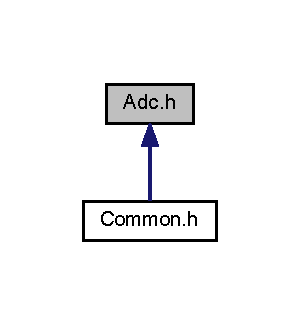
\includegraphics[width=144pt]{_adc_8h__dep__incl}
\end{center}
\end{figure}
\subsection*{Functions}
\begin{DoxyCompactItemize}
\item 
void \hyperlink{_adc_8h_af77988a3ac7a924b75e6213631b04d46}{adc\-Soc\-Cnf} (void)
\item 
void \hyperlink{_adc_8h_a3c614312b1f0ce65b46c4d93051de836}{adc\-Macro\-Configure} (void)
\item 
void \hyperlink{_adc_8h_a646e6cc4558594a6fbaa10c767cc4fec}{adc\-Comp\-Configure} (void)
\item 
Uint16 \hyperlink{_adc_8h_a7dfbe5e2625efeeb0768d42d83a71c04}{adc\-Check\-Ocp} (void)
\item 
Uint16 \hyperlink{_adc_8h_a0ad871be22e7987be07a0f4534ef231b}{adc\-Check\-Ovp} (void)
\item 
Uint16 \hyperlink{_adc_8h_aca1e33ca1b293964f5ce58d430e684f0}{adc\-Set\-Dac} (Uint16 chnl, float32 dac\-Lvl)
\item 
Uint16 \hyperlink{_adc_8h_a2dcc5ee51599a4026fc672072a3f8232}{adc\-Set\-I\-Scale} (Uint16 chnl, float32 scale\-Setting)
\item 
Uint16 \hyperlink{_adc_8h_a9c87603c2aabc17d784a9149563e71e5}{adc\-Set\-V\-Scale} (Uint16 chnl, float32 scale\-Setting)
\item 
Uint16 \hyperlink{_adc_8h_ac5c13a2ef6c3a9f9da7bf437e0213da2}{adc\-Set\-Ocp} (Uint16 chnl, float32 ocp\-Setting)
\item 
Uint16 \hyperlink{_adc_8h_a03e263230a1a25337050bfde1172d1a1}{adc\-Set\-Ovp} (Uint16 chnl, float32 ovp\-Setting)
\item 
Uint16 \hyperlink{_adc_8h_a51b43d0fbadcb3b231f4fceb4c7b9d12}{adc\-Get\-Dac} (Uint16 chnl, float32 $\ast$dac\-Dest)
\item 
Uint16 \hyperlink{_adc_8h_acbf7c83ae3b6df7b0812ef1aed2b9c96}{adc\-Get\-I\-Scale} (Uint16 chnl, float32 $\ast$scl\-Dest)
\item 
Uint16 \hyperlink{_adc_8h_a478f6261679944822575231af3eb229c}{adc\-Get\-V\-Scale} (Uint16 chnl, float32 $\ast$scl\-Dest)
\item 
Uint16 \hyperlink{_adc_8h_a47082a746494c4221df1cb453fa746f7}{adc\-Get\-Voltage} (Uint16 chnl, float32 $\ast$v\-Dest)
\item 
Uint16 \hyperlink{_adc_8h_a2cda2df7670a029f25848b9fe6f37bf8}{adc\-Get\-Current} (Uint16 chnl, float32 $\ast$i\-Dest)
\item 
Uint16 \hyperlink{_adc_8h_a8e08c745a25782602c5d337d5eb7b03c}{adc\-Get\-Ocp} (Uint16 chnl, float32 $\ast$ocp\-Dest)
\item 
Uint16 \hyperlink{_adc_8h_a1536739f53a776036e1b9c92990a102a}{adc\-Get\-Ovp} (Uint16 chnl, float32 $\ast$ovp\-Dest)
\end{DoxyCompactItemize}
\subsection*{Variables}
\begin{DoxyCompactItemize}
\item 
volatile int32 $\ast$ \hyperlink{_adc_8h_a42ca9720519e1d0cb7ded4f56da083ba}{A\-D\-C\-D\-R\-V\-\_\-1ch\-\_\-\-Rlt1}
\item 
volatile int32 $\ast$ \hyperlink{_adc_8h_a1ca55c7841c3e4bc154789647a068810}{A\-D\-C\-D\-R\-V\-\_\-1ch\-\_\-\-Rlt2}
\item 
volatile int32 $\ast$ \hyperlink{_adc_8h_a1704632b071d0fff6bdc9629549c5d08}{A\-D\-C\-D\-R\-V\-\_\-1ch\-\_\-\-Rlt3}
\item 
volatile int32 $\ast$ \hyperlink{_adc_8h_ac181cb2fb372cceb0f55844ed941c5d0}{A\-D\-C\-D\-R\-V\-\_\-1ch\-\_\-\-Rlt4}
\item 
volatile int32 $\ast$ \hyperlink{_adc_8h_a7b586f409f6daf8232917fbd976532a4}{A\-D\-C\-D\-R\-V\-\_\-1ch\-\_\-\-Rlt5}
\item 
volatile int32 $\ast$ \hyperlink{_adc_8h_ae8182c9b35af2d72b1c18ea41ccece2d}{A\-D\-C\-D\-R\-V\-\_\-1ch\-\_\-\-Rlt6}
\item 
volatile int32 $\ast$ \hyperlink{_adc_8h_a4fa6265d0bf9b69d560d8f9f488b98c1}{A\-D\-C\-D\-R\-V\-\_\-1ch\-\_\-\-Rlt7}
\item 
volatile int32 $\ast$ \hyperlink{_adc_8h_a0415309d16a115f0116a26aeda91aabd}{A\-D\-C\-D\-R\-V\-\_\-1ch\-\_\-\-Rlt8}
\item 
volatile int32 $\ast$ \hyperlink{_adc_8h_adea6b0b8533e0d56a5c6cbac1c1e705f}{A\-D\-C\-D\-R\-V\-\_\-1ch\-\_\-\-Rlt9}
\item 
volatile int32 $\ast$ \hyperlink{_adc_8h_ad1b851523cd317f0910f2db4220f32da}{A\-D\-C\-D\-R\-V\-\_\-1ch\-\_\-\-Rlt10}
\item 
volatile int32 $\ast$ \hyperlink{_adc_8h_ad4435404e2f432a8c3a449dd23cda8f0}{A\-D\-C\-D\-R\-V\-\_\-1ch\-\_\-\-Rlt11}
\item 
volatile int32 $\ast$ \hyperlink{_adc_8h_ac3656f047361723ec883e6ebfe3f026a}{A\-D\-C\-D\-R\-V\-\_\-1ch\-\_\-\-Rlt12}
\item 
volatile int32 $\ast$ \hyperlink{_adc_8h_ad7ef0544a173d3c7883f0e739b7d2096}{A\-D\-C\-D\-R\-V\-\_\-1ch\-\_\-\-Rlt13}
\end{DoxyCompactItemize}


\subsection{Detailed Description}
A\-D\-C, D\-A\-C, comparator and related functions. Requires the modification of the C\-O\-M\-P\-\_\-\-R\-E\-G\-S struct of the D\-S\-P2802x\-\_\-\-Global\-Variable\-Defs in the file D\-S\-P2802x\-\_\-\-Comp.\-h, to allow use of the D\-A\-C\-C\-T\-L and ramp-\/related register unions. Use the equivalent file from the f2903x includes for reference. 

\subsection{Function Documentation}
\hypertarget{_adc_8h_a7dfbe5e2625efeeb0768d42d83a71c04}{\index{Adc.\-h@{Adc.\-h}!adc\-Check\-Ocp@{adc\-Check\-Ocp}}
\index{adc\-Check\-Ocp@{adc\-Check\-Ocp}!Adc.h@{Adc.\-h}}
\subsubsection[{adc\-Check\-Ocp}]{\setlength{\rightskip}{0pt plus 5cm}Uint16 adc\-Check\-Ocp (
\begin{DoxyParamCaption}
\item[{void}]{}
\end{DoxyParamCaption}
)}}\label{_adc_8h_a7dfbe5e2625efeeb0768d42d83a71c04}
Checks the current current sense A\-D\-C readings against the O\-C\-P limits. \begin{DoxyReturn}{Returns}
Error status 
\end{DoxyReturn}
\hypertarget{_adc_8h_a0ad871be22e7987be07a0f4534ef231b}{\index{Adc.\-h@{Adc.\-h}!adc\-Check\-Ovp@{adc\-Check\-Ovp}}
\index{adc\-Check\-Ovp@{adc\-Check\-Ovp}!Adc.h@{Adc.\-h}}
\subsubsection[{adc\-Check\-Ovp}]{\setlength{\rightskip}{0pt plus 5cm}Uint16 adc\-Check\-Ovp (
\begin{DoxyParamCaption}
\item[{void}]{}
\end{DoxyParamCaption}
)}}\label{_adc_8h_a0ad871be22e7987be07a0f4534ef231b}
Checks the current voltage sense A\-D\-C readings against the O\-V\-P limits. \begin{DoxyReturn}{Returns}
Error status 
\end{DoxyReturn}
\hypertarget{_adc_8h_a646e6cc4558594a6fbaa10c767cc4fec}{\index{Adc.\-h@{Adc.\-h}!adc\-Comp\-Configure@{adc\-Comp\-Configure}}
\index{adc\-Comp\-Configure@{adc\-Comp\-Configure}!Adc.h@{Adc.\-h}}
\subsubsection[{adc\-Comp\-Configure}]{\setlength{\rightskip}{0pt plus 5cm}void adc\-Comp\-Configure (
\begin{DoxyParamCaption}
\item[{void}]{}
\end{DoxyParamCaption}
)}}\label{_adc_8h_a646e6cc4558594a6fbaa10c767cc4fec}
Configures the C\-O\-M\-P 1 \& 2 comparators using the internal D\-A\-Cs at inverting inputs.
\begin{DoxyItemize}
\item S\-H\-O\-U\-L\-D be called A\-F\-T\-E\-R \hyperlink{_adc_8h_af77988a3ac7a924b75e6213631b04d46}{adc\-Soc\-Cnf()}.
\item S\-H\-O\-U\-L\-D be called B\-E\-F\-O\-R\-E P\-W\-M\-S (S\-Y\-N\-C) are started.
\item S\-H\-O\-U\-L\-D be called B\-E\-F\-O\-R\-E pwm\-T\-Z\-Configure(). 
\end{DoxyItemize}\hypertarget{_adc_8h_a2cda2df7670a029f25848b9fe6f37bf8}{\index{Adc.\-h@{Adc.\-h}!adc\-Get\-Current@{adc\-Get\-Current}}
\index{adc\-Get\-Current@{adc\-Get\-Current}!Adc.h@{Adc.\-h}}
\subsubsection[{adc\-Get\-Current}]{\setlength{\rightskip}{0pt plus 5cm}Uint16 adc\-Get\-Current (
\begin{DoxyParamCaption}
\item[{Uint16}]{chnl, }
\item[{float32 $\ast$}]{i\-Dest}
\end{DoxyParamCaption}
)}}\label{_adc_8h_a2cda2df7670a029f25848b9fe6f37bf8}
Queries the most recent current reading from the specified channel's associated A\-D\-C. 
\begin{DoxyParams}[1]{Parameters}
\mbox{\tt in}  & {\em chnl} & Specifies the channel number on which the reading is to be queried. \\
\hline
\mbox{\tt out}  & {\em i\-Dest} & Address of the memory location at which to place the query result (amps). \\
\hline
\end{DoxyParams}
\begin{DoxyReturn}{Returns}
Error status. 
\end{DoxyReturn}
\hypertarget{_adc_8h_a51b43d0fbadcb3b231f4fceb4c7b9d12}{\index{Adc.\-h@{Adc.\-h}!adc\-Get\-Dac@{adc\-Get\-Dac}}
\index{adc\-Get\-Dac@{adc\-Get\-Dac}!Adc.h@{Adc.\-h}}
\subsubsection[{adc\-Get\-Dac}]{\setlength{\rightskip}{0pt plus 5cm}Uint16 adc\-Get\-Dac (
\begin{DoxyParamCaption}
\item[{Uint16}]{chnl, }
\item[{float32 $\ast$}]{dac\-Dest}
\end{DoxyParamCaption}
)}}\label{_adc_8h_a51b43d0fbadcb3b231f4fceb4c7b9d12}
Queries the output level setting of the D\-A\-C on the inverting input of the comparators. 
\begin{DoxyParams}[1]{Parameters}
\mbox{\tt in}  & {\em chnl} & Specifies the channel number on which the setting is to be queried. \\
\hline
\mbox{\tt out}  & {\em dac\-Dest} & Address of the memory location at which to place the query result (volts or amps). \\
\hline
\end{DoxyParams}
\begin{DoxyReturn}{Returns}
Error status. 
\end{DoxyReturn}
\hypertarget{_adc_8h_acbf7c83ae3b6df7b0812ef1aed2b9c96}{\index{Adc.\-h@{Adc.\-h}!adc\-Get\-I\-Scale@{adc\-Get\-I\-Scale}}
\index{adc\-Get\-I\-Scale@{adc\-Get\-I\-Scale}!Adc.h@{Adc.\-h}}
\subsubsection[{adc\-Get\-I\-Scale}]{\setlength{\rightskip}{0pt plus 5cm}Uint16 adc\-Get\-I\-Scale (
\begin{DoxyParamCaption}
\item[{Uint16}]{chnl, }
\item[{float32 $\ast$}]{scl\-Dest}
\end{DoxyParamCaption}
)}}\label{_adc_8h_acbf7c83ae3b6df7b0812ef1aed2b9c96}
Queries the current current scaling setting of the specified channel. 
\begin{DoxyParams}[1]{Parameters}
\mbox{\tt in}  & {\em chnl} & Specifies the channel number on which the setting is to be queried. \\
\hline
\mbox{\tt out}  & {\em scl\-Dest} & Address of the memory location at which to place the query result (amps). \\
\hline
\end{DoxyParams}
\begin{DoxyReturn}{Returns}
Error status. 
\end{DoxyReturn}
\hypertarget{_adc_8h_a8e08c745a25782602c5d337d5eb7b03c}{\index{Adc.\-h@{Adc.\-h}!adc\-Get\-Ocp@{adc\-Get\-Ocp}}
\index{adc\-Get\-Ocp@{adc\-Get\-Ocp}!Adc.h@{Adc.\-h}}
\subsubsection[{adc\-Get\-Ocp}]{\setlength{\rightskip}{0pt plus 5cm}Uint16 adc\-Get\-Ocp (
\begin{DoxyParamCaption}
\item[{Uint16}]{chnl, }
\item[{float32 $\ast$}]{ocp\-Dest}
\end{DoxyParamCaption}
)}}\label{_adc_8h_a8e08c745a25782602c5d337d5eb7b03c}
Queries the over current protection setting for the specified channel. 
\begin{DoxyParams}[1]{Parameters}
\mbox{\tt in}  & {\em chnl} & Specifies the channel number on which the setting is to be queried. \\
\hline
\mbox{\tt out}  & {\em ocp\-Dest} & Address of the memory location at which to place the query result (amps). \\
\hline
\end{DoxyParams}
\begin{DoxyReturn}{Returns}
Error status. 
\end{DoxyReturn}
\hypertarget{_adc_8h_a1536739f53a776036e1b9c92990a102a}{\index{Adc.\-h@{Adc.\-h}!adc\-Get\-Ovp@{adc\-Get\-Ovp}}
\index{adc\-Get\-Ovp@{adc\-Get\-Ovp}!Adc.h@{Adc.\-h}}
\subsubsection[{adc\-Get\-Ovp}]{\setlength{\rightskip}{0pt plus 5cm}Uint16 adc\-Get\-Ovp (
\begin{DoxyParamCaption}
\item[{Uint16}]{chnl, }
\item[{float32 $\ast$}]{ovp\-Dest}
\end{DoxyParamCaption}
)}}\label{_adc_8h_a1536739f53a776036e1b9c92990a102a}
Queries the over current protection setting for the specified channel. 
\begin{DoxyParams}[1]{Parameters}
\mbox{\tt in}  & {\em chnl} & Specifies the channel number on which the setting is to be queried. \\
\hline
\mbox{\tt out}  & {\em ovp\-Dest} & Address of the memory location at which to place the query result (volts). \\
\hline
\end{DoxyParams}
\begin{DoxyReturn}{Returns}
Error status. 
\end{DoxyReturn}
\hypertarget{_adc_8h_a47082a746494c4221df1cb453fa746f7}{\index{Adc.\-h@{Adc.\-h}!adc\-Get\-Voltage@{adc\-Get\-Voltage}}
\index{adc\-Get\-Voltage@{adc\-Get\-Voltage}!Adc.h@{Adc.\-h}}
\subsubsection[{adc\-Get\-Voltage}]{\setlength{\rightskip}{0pt plus 5cm}Uint16 adc\-Get\-Voltage (
\begin{DoxyParamCaption}
\item[{Uint16}]{chnl, }
\item[{float32 $\ast$}]{v\-Dest}
\end{DoxyParamCaption}
)}}\label{_adc_8h_a47082a746494c4221df1cb453fa746f7}
Queries the most recent voltage reading from the specified channel's associated A\-D\-C. 
\begin{DoxyParams}[1]{Parameters}
\mbox{\tt in}  & {\em chnl} & Specifies the channel number on which the reading is to be queried. \\
\hline
\mbox{\tt out}  & {\em v\-Dest} & Address of the memory location at which to place the query result (volts). \\
\hline
\end{DoxyParams}
\begin{DoxyReturn}{Returns}
Error status. 
\end{DoxyReturn}
\hypertarget{_adc_8h_a478f6261679944822575231af3eb229c}{\index{Adc.\-h@{Adc.\-h}!adc\-Get\-V\-Scale@{adc\-Get\-V\-Scale}}
\index{adc\-Get\-V\-Scale@{adc\-Get\-V\-Scale}!Adc.h@{Adc.\-h}}
\subsubsection[{adc\-Get\-V\-Scale}]{\setlength{\rightskip}{0pt plus 5cm}Uint16 adc\-Get\-V\-Scale (
\begin{DoxyParamCaption}
\item[{Uint16}]{chnl, }
\item[{float32 $\ast$}]{scl\-Dest}
\end{DoxyParamCaption}
)}}\label{_adc_8h_a478f6261679944822575231af3eb229c}
Queries the current voltage scaling setting of the specified channel. 
\begin{DoxyParams}[1]{Parameters}
\mbox{\tt in}  & {\em chnl} & Specifies the channel number on which the setting is to be queried. \\
\hline
\mbox{\tt out}  & {\em scl\-Dest} & Address of the memory location at which to place the query result (volts). \\
\hline
\end{DoxyParams}
\begin{DoxyReturn}{Returns}
Error status. 
\end{DoxyReturn}
\hypertarget{_adc_8h_a3c614312b1f0ce65b46c4d93051de836}{\index{Adc.\-h@{Adc.\-h}!adc\-Macro\-Configure@{adc\-Macro\-Configure}}
\index{adc\-Macro\-Configure@{adc\-Macro\-Configure}!Adc.h@{Adc.\-h}}
\subsubsection[{adc\-Macro\-Configure}]{\setlength{\rightskip}{0pt plus 5cm}void adc\-Macro\-Configure (
\begin{DoxyParamCaption}
\item[{void}]{}
\end{DoxyParamCaption}
)}}\label{_adc_8h_a3c614312b1f0ce65b46c4d93051de836}
Configures the A\-D\-C's S\-O\-Cs then calls \hyperlink{_pwm_8h_a358d8706acd0faf4e1cc705129be6548}{pwm\-Soc\-Configure()}.
\begin{DoxyItemize}
\item S\-H\-O\-U\-L\-D be run after \hyperlink{_pwm_8h_acc68120fcdfa36145370c31a61eb23a7}{pwm\-Macro\-Configure()}.
\item S\-H\-O\-U\-L\-D be run before D\-P\-L\-\_\-\-I\-N\-I\-T(). 
\end{DoxyItemize}\hypertarget{_adc_8h_aca1e33ca1b293964f5ce58d430e684f0}{\index{Adc.\-h@{Adc.\-h}!adc\-Set\-Dac@{adc\-Set\-Dac}}
\index{adc\-Set\-Dac@{adc\-Set\-Dac}!Adc.h@{Adc.\-h}}
\subsubsection[{adc\-Set\-Dac}]{\setlength{\rightskip}{0pt plus 5cm}Uint16 adc\-Set\-Dac (
\begin{DoxyParamCaption}
\item[{Uint16}]{chnl, }
\item[{float32}]{dac\-Lvl}
\end{DoxyParamCaption}
)}}\label{_adc_8h_aca1e33ca1b293964f5ce58d430e684f0}
Sets the output levels of the D\-A\-Cs on the inverting input of the comparators. The function will determine the scaling to be applied by testing the ctrl\-Mode setting of the channel specified. The respective channel's current or voltage M\-U\-S\-T be set previously. 
\begin{DoxyParams}[1]{Parameters}
\mbox{\tt in}  & {\em chnl} & Specifies the channel number the setting is to be applied to. \\
\hline
\mbox{\tt in}  & {\em dac\-Lvl} & Specifies the value of the level setting to be applied (volts or amps). \\
\hline
\end{DoxyParams}
\begin{DoxyReturn}{Returns}
Error status. 
\end{DoxyReturn}
\hypertarget{_adc_8h_a2dcc5ee51599a4026fc672072a3f8232}{\index{Adc.\-h@{Adc.\-h}!adc\-Set\-I\-Scale@{adc\-Set\-I\-Scale}}
\index{adc\-Set\-I\-Scale@{adc\-Set\-I\-Scale}!Adc.h@{Adc.\-h}}
\subsubsection[{adc\-Set\-I\-Scale}]{\setlength{\rightskip}{0pt plus 5cm}Uint16 adc\-Set\-I\-Scale (
\begin{DoxyParamCaption}
\item[{Uint16}]{chnl, }
\item[{float32}]{scale\-Setting}
\end{DoxyParamCaption}
)}}\label{_adc_8h_a2dcc5ee51599a4026fc672072a3f8232}
Sets the current scaling for the specified channel. 
\begin{DoxyParams}[1]{Parameters}
\mbox{\tt in}  & {\em chnl} & Specifies the channel number the setting is to be applied to. \\
\hline
\mbox{\tt in}  & {\em scale\-Setting} & Specifies the value of the scaling setting to be applied (amps/volts). \\
\hline
\end{DoxyParams}
\begin{DoxyReturn}{Returns}
Error status. 
\end{DoxyReturn}
\hypertarget{_adc_8h_ac5c13a2ef6c3a9f9da7bf437e0213da2}{\index{Adc.\-h@{Adc.\-h}!adc\-Set\-Ocp@{adc\-Set\-Ocp}}
\index{adc\-Set\-Ocp@{adc\-Set\-Ocp}!Adc.h@{Adc.\-h}}
\subsubsection[{adc\-Set\-Ocp}]{\setlength{\rightskip}{0pt plus 5cm}Uint16 adc\-Set\-Ocp (
\begin{DoxyParamCaption}
\item[{Uint16}]{chnl, }
\item[{float32}]{ocp\-Setting}
\end{DoxyParamCaption}
)}}\label{_adc_8h_ac5c13a2ef6c3a9f9da7bf437e0213da2}
Sets the over current protection limit for the specified channel. 
\begin{DoxyParams}[1]{Parameters}
\mbox{\tt in}  & {\em chnl} & Specifies the channel number the setting is to be applied to. \\
\hline
\mbox{\tt in}  & {\em ocp\-Setting} & Specifies the value of the limit to be applied (Amps). \\
\hline
\end{DoxyParams}
\begin{DoxyReturn}{Returns}
Error status. 
\end{DoxyReturn}
\hypertarget{_adc_8h_a03e263230a1a25337050bfde1172d1a1}{\index{Adc.\-h@{Adc.\-h}!adc\-Set\-Ovp@{adc\-Set\-Ovp}}
\index{adc\-Set\-Ovp@{adc\-Set\-Ovp}!Adc.h@{Adc.\-h}}
\subsubsection[{adc\-Set\-Ovp}]{\setlength{\rightskip}{0pt plus 5cm}Uint16 adc\-Set\-Ovp (
\begin{DoxyParamCaption}
\item[{Uint16}]{chnl, }
\item[{float32}]{ovp\-Setting}
\end{DoxyParamCaption}
)}}\label{_adc_8h_a03e263230a1a25337050bfde1172d1a1}
Sets the over voltage protection limit for the specified channel. 
\begin{DoxyParams}[1]{Parameters}
\mbox{\tt in}  & {\em chnl} & Specifies the channel number the setting is to be applied to. \\
\hline
\mbox{\tt in}  & {\em ovp\-Setting} & Specifies the value of the limit to be applied (volts). \\
\hline
\end{DoxyParams}
\begin{DoxyReturn}{Returns}
Error status. 
\end{DoxyReturn}
\hypertarget{_adc_8h_a9c87603c2aabc17d784a9149563e71e5}{\index{Adc.\-h@{Adc.\-h}!adc\-Set\-V\-Scale@{adc\-Set\-V\-Scale}}
\index{adc\-Set\-V\-Scale@{adc\-Set\-V\-Scale}!Adc.h@{Adc.\-h}}
\subsubsection[{adc\-Set\-V\-Scale}]{\setlength{\rightskip}{0pt plus 5cm}Uint16 adc\-Set\-V\-Scale (
\begin{DoxyParamCaption}
\item[{Uint16}]{chnl, }
\item[{float32}]{scale\-Setting}
\end{DoxyParamCaption}
)}}\label{_adc_8h_a9c87603c2aabc17d784a9149563e71e5}
Sets the voltage scaling for the specified channel. 
\begin{DoxyParams}[1]{Parameters}
\mbox{\tt in}  & {\em chnl} & Specifies the channel number the setting is to be applied to. \\
\hline
\mbox{\tt in}  & {\em scale\-Setting} & Specifies the value of the scaling setting to be applied (volts/volts). \\
\hline
\end{DoxyParams}
\begin{DoxyReturn}{Returns}
Error status. 
\end{DoxyReturn}
\hypertarget{_adc_8h_af77988a3ac7a924b75e6213631b04d46}{\index{Adc.\-h@{Adc.\-h}!adc\-Soc\-Cnf@{adc\-Soc\-Cnf}}
\index{adc\-Soc\-Cnf@{adc\-Soc\-Cnf}!Adc.h@{Adc.\-h}}
\subsubsection[{adc\-Soc\-Cnf}]{\setlength{\rightskip}{0pt plus 5cm}void adc\-Soc\-Cnf (
\begin{DoxyParamCaption}
\item[{void}]{}
\end{DoxyParamCaption}
)}}\label{_adc_8h_af77988a3ac7a924b75e6213631b04d46}
Configures A\-D\-C S\-O\-C for A\-D\-C macro 

\subsection{Variable Documentation}
\hypertarget{_adc_8h_a42ca9720519e1d0cb7ded4f56da083ba}{\index{Adc.\-h@{Adc.\-h}!A\-D\-C\-D\-R\-V\-\_\-1ch\-\_\-\-Rlt1@{A\-D\-C\-D\-R\-V\-\_\-1ch\-\_\-\-Rlt1}}
\index{A\-D\-C\-D\-R\-V\-\_\-1ch\-\_\-\-Rlt1@{A\-D\-C\-D\-R\-V\-\_\-1ch\-\_\-\-Rlt1}!Adc.h@{Adc.\-h}}
\subsubsection[{A\-D\-C\-D\-R\-V\-\_\-1ch\-\_\-\-Rlt1}]{\setlength{\rightskip}{0pt plus 5cm}volatile int32$\ast$ A\-D\-C\-D\-R\-V\-\_\-1ch\-\_\-\-Rlt1}}\label{_adc_8h_a42ca9720519e1d0cb7ded4f56da083ba}
Channel 0 current sense A\-D\-C terminal pointer. \hypertarget{_adc_8h_ad1b851523cd317f0910f2db4220f32da}{\index{Adc.\-h@{Adc.\-h}!A\-D\-C\-D\-R\-V\-\_\-1ch\-\_\-\-Rlt10@{A\-D\-C\-D\-R\-V\-\_\-1ch\-\_\-\-Rlt10}}
\index{A\-D\-C\-D\-R\-V\-\_\-1ch\-\_\-\-Rlt10@{A\-D\-C\-D\-R\-V\-\_\-1ch\-\_\-\-Rlt10}!Adc.h@{Adc.\-h}}
\subsubsection[{A\-D\-C\-D\-R\-V\-\_\-1ch\-\_\-\-Rlt10}]{\setlength{\rightskip}{0pt plus 5cm}volatile int32$\ast$ A\-D\-C\-D\-R\-V\-\_\-1ch\-\_\-\-Rlt10}}\label{_adc_8h_ad1b851523cd317f0910f2db4220f32da}
Channel 3 voltage sense A\-D\-C terminal pointer. \hypertarget{_adc_8h_ad4435404e2f432a8c3a449dd23cda8f0}{\index{Adc.\-h@{Adc.\-h}!A\-D\-C\-D\-R\-V\-\_\-1ch\-\_\-\-Rlt11@{A\-D\-C\-D\-R\-V\-\_\-1ch\-\_\-\-Rlt11}}
\index{A\-D\-C\-D\-R\-V\-\_\-1ch\-\_\-\-Rlt11@{A\-D\-C\-D\-R\-V\-\_\-1ch\-\_\-\-Rlt11}!Adc.h@{Adc.\-h}}
\subsubsection[{A\-D\-C\-D\-R\-V\-\_\-1ch\-\_\-\-Rlt11}]{\setlength{\rightskip}{0pt plus 5cm}volatile int32$\ast$ A\-D\-C\-D\-R\-V\-\_\-1ch\-\_\-\-Rlt11}}\label{_adc_8h_ad4435404e2f432a8c3a449dd23cda8f0}
Interboost voltage sense A\-D\-C terminal pointer. \hypertarget{_adc_8h_ac3656f047361723ec883e6ebfe3f026a}{\index{Adc.\-h@{Adc.\-h}!A\-D\-C\-D\-R\-V\-\_\-1ch\-\_\-\-Rlt12@{A\-D\-C\-D\-R\-V\-\_\-1ch\-\_\-\-Rlt12}}
\index{A\-D\-C\-D\-R\-V\-\_\-1ch\-\_\-\-Rlt12@{A\-D\-C\-D\-R\-V\-\_\-1ch\-\_\-\-Rlt12}!Adc.h@{Adc.\-h}}
\subsubsection[{A\-D\-C\-D\-R\-V\-\_\-1ch\-\_\-\-Rlt12}]{\setlength{\rightskip}{0pt plus 5cm}volatile int32$\ast$ A\-D\-C\-D\-R\-V\-\_\-1ch\-\_\-\-Rlt12}}\label{_adc_8h_ac3656f047361723ec883e6ebfe3f026a}
A\-C stage voltage sense A\-D\-C terminal pointer. \hypertarget{_adc_8h_ad7ef0544a173d3c7883f0e739b7d2096}{\index{Adc.\-h@{Adc.\-h}!A\-D\-C\-D\-R\-V\-\_\-1ch\-\_\-\-Rlt13@{A\-D\-C\-D\-R\-V\-\_\-1ch\-\_\-\-Rlt13}}
\index{A\-D\-C\-D\-R\-V\-\_\-1ch\-\_\-\-Rlt13@{A\-D\-C\-D\-R\-V\-\_\-1ch\-\_\-\-Rlt13}!Adc.h@{Adc.\-h}}
\subsubsection[{A\-D\-C\-D\-R\-V\-\_\-1ch\-\_\-\-Rlt13}]{\setlength{\rightskip}{0pt plus 5cm}volatile int32$\ast$ A\-D\-C\-D\-R\-V\-\_\-1ch\-\_\-\-Rlt13}}\label{_adc_8h_ad7ef0544a173d3c7883f0e739b7d2096}
V\-Mid voltage sense A\-D\-C terminal pointer. \hypertarget{_adc_8h_a1ca55c7841c3e4bc154789647a068810}{\index{Adc.\-h@{Adc.\-h}!A\-D\-C\-D\-R\-V\-\_\-1ch\-\_\-\-Rlt2@{A\-D\-C\-D\-R\-V\-\_\-1ch\-\_\-\-Rlt2}}
\index{A\-D\-C\-D\-R\-V\-\_\-1ch\-\_\-\-Rlt2@{A\-D\-C\-D\-R\-V\-\_\-1ch\-\_\-\-Rlt2}!Adc.h@{Adc.\-h}}
\subsubsection[{A\-D\-C\-D\-R\-V\-\_\-1ch\-\_\-\-Rlt2}]{\setlength{\rightskip}{0pt plus 5cm}volatile int32$\ast$ A\-D\-C\-D\-R\-V\-\_\-1ch\-\_\-\-Rlt2}}\label{_adc_8h_a1ca55c7841c3e4bc154789647a068810}
Channel 1 current sense A\-D\-C terminal pointer. \hypertarget{_adc_8h_a1704632b071d0fff6bdc9629549c5d08}{\index{Adc.\-h@{Adc.\-h}!A\-D\-C\-D\-R\-V\-\_\-1ch\-\_\-\-Rlt3@{A\-D\-C\-D\-R\-V\-\_\-1ch\-\_\-\-Rlt3}}
\index{A\-D\-C\-D\-R\-V\-\_\-1ch\-\_\-\-Rlt3@{A\-D\-C\-D\-R\-V\-\_\-1ch\-\_\-\-Rlt3}!Adc.h@{Adc.\-h}}
\subsubsection[{A\-D\-C\-D\-R\-V\-\_\-1ch\-\_\-\-Rlt3}]{\setlength{\rightskip}{0pt plus 5cm}volatile int32$\ast$ A\-D\-C\-D\-R\-V\-\_\-1ch\-\_\-\-Rlt3}}\label{_adc_8h_a1704632b071d0fff6bdc9629549c5d08}
Channel 2 current sense A\-D\-C terminal pointer. \hypertarget{_adc_8h_ac181cb2fb372cceb0f55844ed941c5d0}{\index{Adc.\-h@{Adc.\-h}!A\-D\-C\-D\-R\-V\-\_\-1ch\-\_\-\-Rlt4@{A\-D\-C\-D\-R\-V\-\_\-1ch\-\_\-\-Rlt4}}
\index{A\-D\-C\-D\-R\-V\-\_\-1ch\-\_\-\-Rlt4@{A\-D\-C\-D\-R\-V\-\_\-1ch\-\_\-\-Rlt4}!Adc.h@{Adc.\-h}}
\subsubsection[{A\-D\-C\-D\-R\-V\-\_\-1ch\-\_\-\-Rlt4}]{\setlength{\rightskip}{0pt plus 5cm}volatile int32$\ast$ A\-D\-C\-D\-R\-V\-\_\-1ch\-\_\-\-Rlt4}}\label{_adc_8h_ac181cb2fb372cceb0f55844ed941c5d0}
Channel 3 current sense A\-D\-C terminal pointer. \hypertarget{_adc_8h_a7b586f409f6daf8232917fbd976532a4}{\index{Adc.\-h@{Adc.\-h}!A\-D\-C\-D\-R\-V\-\_\-1ch\-\_\-\-Rlt5@{A\-D\-C\-D\-R\-V\-\_\-1ch\-\_\-\-Rlt5}}
\index{A\-D\-C\-D\-R\-V\-\_\-1ch\-\_\-\-Rlt5@{A\-D\-C\-D\-R\-V\-\_\-1ch\-\_\-\-Rlt5}!Adc.h@{Adc.\-h}}
\subsubsection[{A\-D\-C\-D\-R\-V\-\_\-1ch\-\_\-\-Rlt5}]{\setlength{\rightskip}{0pt plus 5cm}volatile int32$\ast$ A\-D\-C\-D\-R\-V\-\_\-1ch\-\_\-\-Rlt5}}\label{_adc_8h_a7b586f409f6daf8232917fbd976532a4}
Interboost current sense A\-D\-C terminal pointer. \hypertarget{_adc_8h_ae8182c9b35af2d72b1c18ea41ccece2d}{\index{Adc.\-h@{Adc.\-h}!A\-D\-C\-D\-R\-V\-\_\-1ch\-\_\-\-Rlt6@{A\-D\-C\-D\-R\-V\-\_\-1ch\-\_\-\-Rlt6}}
\index{A\-D\-C\-D\-R\-V\-\_\-1ch\-\_\-\-Rlt6@{A\-D\-C\-D\-R\-V\-\_\-1ch\-\_\-\-Rlt6}!Adc.h@{Adc.\-h}}
\subsubsection[{A\-D\-C\-D\-R\-V\-\_\-1ch\-\_\-\-Rlt6}]{\setlength{\rightskip}{0pt plus 5cm}volatile int32$\ast$ A\-D\-C\-D\-R\-V\-\_\-1ch\-\_\-\-Rlt6}}\label{_adc_8h_ae8182c9b35af2d72b1c18ea41ccece2d}
A\-C stage current sense A\-D\-C terminal pointer. \hypertarget{_adc_8h_a4fa6265d0bf9b69d560d8f9f488b98c1}{\index{Adc.\-h@{Adc.\-h}!A\-D\-C\-D\-R\-V\-\_\-1ch\-\_\-\-Rlt7@{A\-D\-C\-D\-R\-V\-\_\-1ch\-\_\-\-Rlt7}}
\index{A\-D\-C\-D\-R\-V\-\_\-1ch\-\_\-\-Rlt7@{A\-D\-C\-D\-R\-V\-\_\-1ch\-\_\-\-Rlt7}!Adc.h@{Adc.\-h}}
\subsubsection[{A\-D\-C\-D\-R\-V\-\_\-1ch\-\_\-\-Rlt7}]{\setlength{\rightskip}{0pt plus 5cm}volatile int32$\ast$ A\-D\-C\-D\-R\-V\-\_\-1ch\-\_\-\-Rlt7}}\label{_adc_8h_a4fa6265d0bf9b69d560d8f9f488b98c1}
Channel 0 voltage sense A\-D\-C terminal pointer. \hypertarget{_adc_8h_a0415309d16a115f0116a26aeda91aabd}{\index{Adc.\-h@{Adc.\-h}!A\-D\-C\-D\-R\-V\-\_\-1ch\-\_\-\-Rlt8@{A\-D\-C\-D\-R\-V\-\_\-1ch\-\_\-\-Rlt8}}
\index{A\-D\-C\-D\-R\-V\-\_\-1ch\-\_\-\-Rlt8@{A\-D\-C\-D\-R\-V\-\_\-1ch\-\_\-\-Rlt8}!Adc.h@{Adc.\-h}}
\subsubsection[{A\-D\-C\-D\-R\-V\-\_\-1ch\-\_\-\-Rlt8}]{\setlength{\rightskip}{0pt plus 5cm}volatile int32$\ast$ A\-D\-C\-D\-R\-V\-\_\-1ch\-\_\-\-Rlt8}}\label{_adc_8h_a0415309d16a115f0116a26aeda91aabd}
Channel 1 voltage sense A\-D\-C terminal pointer. \hypertarget{_adc_8h_adea6b0b8533e0d56a5c6cbac1c1e705f}{\index{Adc.\-h@{Adc.\-h}!A\-D\-C\-D\-R\-V\-\_\-1ch\-\_\-\-Rlt9@{A\-D\-C\-D\-R\-V\-\_\-1ch\-\_\-\-Rlt9}}
\index{A\-D\-C\-D\-R\-V\-\_\-1ch\-\_\-\-Rlt9@{A\-D\-C\-D\-R\-V\-\_\-1ch\-\_\-\-Rlt9}!Adc.h@{Adc.\-h}}
\subsubsection[{A\-D\-C\-D\-R\-V\-\_\-1ch\-\_\-\-Rlt9}]{\setlength{\rightskip}{0pt plus 5cm}volatile int32$\ast$ A\-D\-C\-D\-R\-V\-\_\-1ch\-\_\-\-Rlt9}}\label{_adc_8h_adea6b0b8533e0d56a5c6cbac1c1e705f}
Channel 2 voltage sense A\-D\-C terminal pointer. 
\hypertarget{_bst_en_8h}{\section{Bst\-En.\-h File Reference}
\label{_bst_en_8h}\index{Bst\-En.\-h@{Bst\-En.\-h}}
}


Functions for enabling and disabling the boost converter stages via I2\-C.  


This graph shows which files directly or indirectly include this file\-:\nopagebreak
\begin{figure}[H]
\begin{center}
\leavevmode
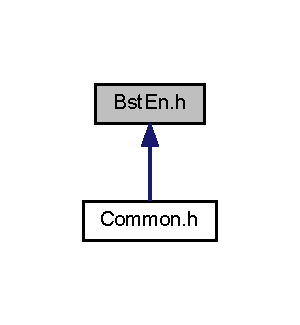
\includegraphics[width=144pt]{_bst_en_8h__dep__incl}
\end{center}
\end{figure}
\subsection*{Macros}
\begin{DoxyCompactItemize}
\item 
\#define \hyperlink{_bst_en_8h_ad615a329bea187ce779cf9930ba8a6fa}{I\-O\-E\-\_\-\-I2\-C\-\_\-\-A\-D\-D\-R}~0x20
\item 
\#define \hyperlink{_bst_en_8h_a36c134b088cc2e64e0a5e14e8f90fe38}{I\-O\-E\-\_\-\-I\-O\-D\-I\-R\-\_\-\-A\-D\-D\-R}~0x00
\item 
\#define \hyperlink{_bst_en_8h_a04633cd2ea7fd0b332e1edf066f674c4}{I\-O\-E\-\_\-\-I\-P\-O\-L\-\_\-\-A\-D\-D\-R}~0x01
\item 
\#define \hyperlink{_bst_en_8h_aa68be5a6ed28fb146600b4fd2d11fafd}{I\-O\-E\-\_\-\-G\-P\-I\-N\-T\-E\-N\-\_\-\-A\-D\-D\-R}~0x02
\item 
\#define \hyperlink{_bst_en_8h_a687e15212e8d4b49c12159dce73eeeab}{I\-O\-E\-\_\-\-D\-E\-F\-V\-A\-L\-\_\-\-A\-D\-D\-R}~0x03
\item 
\#define \hyperlink{_bst_en_8h_a90945d9544eebc892154f1e0443b1407}{I\-O\-E\-\_\-\-I\-N\-T\-C\-O\-N\-\_\-\-A\-D\-D\-R}~0x04
\item 
\#define \hyperlink{_bst_en_8h_af44ed2bf93808aeb932ce9944a942b75}{I\-O\-E\-\_\-\-I\-O\-C\-O\-N\-\_\-\-A\-D\-D\-R}~0x05
\item 
\#define \hyperlink{_bst_en_8h_a91e588d697383f94de2bf7f11d9ecb4b}{I\-O\-E\-\_\-\-G\-P\-P\-U\-\_\-\-A\-D\-D\-R}~0x06
\item 
\#define \hyperlink{_bst_en_8h_a32cac2ad5af58a2562540ec8fc205dd1}{I\-O\-E\-\_\-\-I\-N\-T\-F\-\_\-\-A\-D\-D\-R}~0x07
\item 
\#define \hyperlink{_bst_en_8h_ac0afd8503a8584599cc81f3d9b0a04dc}{I\-O\-E\-\_\-\-I\-N\-T\-C\-A\-P\-\_\-\-A\-D\-D\-R}~0x08
\item 
\#define \hyperlink{_bst_en_8h_af2d85152c5775a221f107d6de547bca1}{I\-O\-E\-\_\-\-G\-P\-I\-O\-\_\-\-A\-D\-D\-R}~0x09
\item 
\#define \hyperlink{_bst_en_8h_ab26864d7372ac11db9c1996842a3cf56}{I\-O\-E\-\_\-\-O\-L\-A\-T\-\_\-\-A\-D\-D\-R}~0x0\-A
\item 
\#define \hyperlink{_bst_en_8h_ac36a77a8d07d8025000e3e748cea40dd}{B\-S\-T\-\_\-\-N\-U\-M\-\_\-\-C\-H\-N\-L}~0x04
\item 
\#define \hyperlink{_bst_en_8h_a5b329f52cf0129bf56d1b16eb706dee4}{I\-O\-E\-\_\-\-N\-U\-M\-\_\-\-C\-H\-N\-L}~\hyperlink{_bst_en_8h_ac36a77a8d07d8025000e3e748cea40dd}{B\-S\-T\-\_\-\-N\-U\-M\-\_\-\-C\-H\-N\-L}
\end{DoxyCompactItemize}
\subsection*{Functions}
\begin{DoxyCompactItemize}
\item 
Uint16 \hyperlink{_bst_en_8h_aa6cb02a7aacce8671212b21ed6e39863}{bc\-Init} (void)
\item 
Uint16 \hyperlink{_bst_en_8h_af10c5e095b6142ee37930042bd1da708}{bc\-Enable} (Uint16 chnl)
\item 
Uint16 \hyperlink{_bst_en_8h_a3df6954c93c9089cdc750fff4b89da3e}{bc\-Disable} (Uint16 chnl)
\end{DoxyCompactItemize}


\subsection{Detailed Description}
Functions for enabling and disabling the boost converter stages via I2\-C. The converters are controlled via an external I/\-O expander (M\-C\-P23008) that is connected to the I2\-C bus at address 0100x-\/x-\/x where 'x-\/x-\/x' is dependent upon the configuration of resistors R60 -\/ 61 \& R70 -\/ R74.

After \hyperlink{_bst_en_8h_aa6cb02a7aacce8671212b21ed6e39863}{bc\-Init()} all converters default to disabled.

\begin{DoxyWarning}{Warning}
Before any converter control functions can be used the I2\-C peripheral M\-U\-S\-T be initialised and E\-I\-T\-H\-E\-R \hyperlink{_bst_en_8h_aa6cb02a7aacce8671212b21ed6e39863}{bc\-Init()} or \hyperlink{_fan_en_8h_a3506b5e25346351ce292e2ad256607cc}{fc\-Init()} M\-U\-S\-T be run -\/ \hyperlink{_bst_en_8h_aa6cb02a7aacce8671212b21ed6e39863}{bc\-Init()} will require the interrupts to be enabled globally.
\end{DoxyWarning}
\begin{DoxySeeAlso}{See Also}
\hyperlink{_i2c_8h_a1e0a81a1ad1fd7710ca189236e3e5476}{i2c\-Init()} 

\hyperlink{_fan_en_8h_a3506b5e25346351ce292e2ad256607cc}{fc\-Init()} 
\end{DoxySeeAlso}


\subsection{Macro Definition Documentation}
\hypertarget{_bst_en_8h_ac36a77a8d07d8025000e3e748cea40dd}{\index{Bst\-En.\-h@{Bst\-En.\-h}!B\-S\-T\-\_\-\-N\-U\-M\-\_\-\-C\-H\-N\-L@{B\-S\-T\-\_\-\-N\-U\-M\-\_\-\-C\-H\-N\-L}}
\index{B\-S\-T\-\_\-\-N\-U\-M\-\_\-\-C\-H\-N\-L@{B\-S\-T\-\_\-\-N\-U\-M\-\_\-\-C\-H\-N\-L}!BstEn.h@{Bst\-En.\-h}}
\subsubsection[{B\-S\-T\-\_\-\-N\-U\-M\-\_\-\-C\-H\-N\-L}]{\setlength{\rightskip}{0pt plus 5cm}\#define B\-S\-T\-\_\-\-N\-U\-M\-\_\-\-C\-H\-N\-L~0x04}}\label{_bst_en_8h_ac36a77a8d07d8025000e3e748cea40dd}
Number of boost converter channels. \hypertarget{_bst_en_8h_a687e15212e8d4b49c12159dce73eeeab}{\index{Bst\-En.\-h@{Bst\-En.\-h}!I\-O\-E\-\_\-\-D\-E\-F\-V\-A\-L\-\_\-\-A\-D\-D\-R@{I\-O\-E\-\_\-\-D\-E\-F\-V\-A\-L\-\_\-\-A\-D\-D\-R}}
\index{I\-O\-E\-\_\-\-D\-E\-F\-V\-A\-L\-\_\-\-A\-D\-D\-R@{I\-O\-E\-\_\-\-D\-E\-F\-V\-A\-L\-\_\-\-A\-D\-D\-R}!BstEn.h@{Bst\-En.\-h}}
\subsubsection[{I\-O\-E\-\_\-\-D\-E\-F\-V\-A\-L\-\_\-\-A\-D\-D\-R}]{\setlength{\rightskip}{0pt plus 5cm}\#define I\-O\-E\-\_\-\-D\-E\-F\-V\-A\-L\-\_\-\-A\-D\-D\-R~0x03}}\label{_bst_en_8h_a687e15212e8d4b49c12159dce73eeeab}
M\-C\-P23008 I/\-O expander default value register address. \hypertarget{_bst_en_8h_aa68be5a6ed28fb146600b4fd2d11fafd}{\index{Bst\-En.\-h@{Bst\-En.\-h}!I\-O\-E\-\_\-\-G\-P\-I\-N\-T\-E\-N\-\_\-\-A\-D\-D\-R@{I\-O\-E\-\_\-\-G\-P\-I\-N\-T\-E\-N\-\_\-\-A\-D\-D\-R}}
\index{I\-O\-E\-\_\-\-G\-P\-I\-N\-T\-E\-N\-\_\-\-A\-D\-D\-R@{I\-O\-E\-\_\-\-G\-P\-I\-N\-T\-E\-N\-\_\-\-A\-D\-D\-R}!BstEn.h@{Bst\-En.\-h}}
\subsubsection[{I\-O\-E\-\_\-\-G\-P\-I\-N\-T\-E\-N\-\_\-\-A\-D\-D\-R}]{\setlength{\rightskip}{0pt plus 5cm}\#define I\-O\-E\-\_\-\-G\-P\-I\-N\-T\-E\-N\-\_\-\-A\-D\-D\-R~0x02}}\label{_bst_en_8h_aa68be5a6ed28fb146600b4fd2d11fafd}
M\-C\-P23008 I/\-O expander interrupt on change enable register address. \hypertarget{_bst_en_8h_af2d85152c5775a221f107d6de547bca1}{\index{Bst\-En.\-h@{Bst\-En.\-h}!I\-O\-E\-\_\-\-G\-P\-I\-O\-\_\-\-A\-D\-D\-R@{I\-O\-E\-\_\-\-G\-P\-I\-O\-\_\-\-A\-D\-D\-R}}
\index{I\-O\-E\-\_\-\-G\-P\-I\-O\-\_\-\-A\-D\-D\-R@{I\-O\-E\-\_\-\-G\-P\-I\-O\-\_\-\-A\-D\-D\-R}!BstEn.h@{Bst\-En.\-h}}
\subsubsection[{I\-O\-E\-\_\-\-G\-P\-I\-O\-\_\-\-A\-D\-D\-R}]{\setlength{\rightskip}{0pt plus 5cm}\#define I\-O\-E\-\_\-\-G\-P\-I\-O\-\_\-\-A\-D\-D\-R~0x09}}\label{_bst_en_8h_af2d85152c5775a221f107d6de547bca1}
M\-C\-P23008 I/\-O expander G\-P\-I\-O port register address. \hypertarget{_bst_en_8h_a91e588d697383f94de2bf7f11d9ecb4b}{\index{Bst\-En.\-h@{Bst\-En.\-h}!I\-O\-E\-\_\-\-G\-P\-P\-U\-\_\-\-A\-D\-D\-R@{I\-O\-E\-\_\-\-G\-P\-P\-U\-\_\-\-A\-D\-D\-R}}
\index{I\-O\-E\-\_\-\-G\-P\-P\-U\-\_\-\-A\-D\-D\-R@{I\-O\-E\-\_\-\-G\-P\-P\-U\-\_\-\-A\-D\-D\-R}!BstEn.h@{Bst\-En.\-h}}
\subsubsection[{I\-O\-E\-\_\-\-G\-P\-P\-U\-\_\-\-A\-D\-D\-R}]{\setlength{\rightskip}{0pt plus 5cm}\#define I\-O\-E\-\_\-\-G\-P\-P\-U\-\_\-\-A\-D\-D\-R~0x06}}\label{_bst_en_8h_a91e588d697383f94de2bf7f11d9ecb4b}
M\-C\-P23008 I/\-O expander pull-\/up resistor configuration register address. \hypertarget{_bst_en_8h_ad615a329bea187ce779cf9930ba8a6fa}{\index{Bst\-En.\-h@{Bst\-En.\-h}!I\-O\-E\-\_\-\-I2\-C\-\_\-\-A\-D\-D\-R@{I\-O\-E\-\_\-\-I2\-C\-\_\-\-A\-D\-D\-R}}
\index{I\-O\-E\-\_\-\-I2\-C\-\_\-\-A\-D\-D\-R@{I\-O\-E\-\_\-\-I2\-C\-\_\-\-A\-D\-D\-R}!BstEn.h@{Bst\-En.\-h}}
\subsubsection[{I\-O\-E\-\_\-\-I2\-C\-\_\-\-A\-D\-D\-R}]{\setlength{\rightskip}{0pt plus 5cm}\#define I\-O\-E\-\_\-\-I2\-C\-\_\-\-A\-D\-D\-R~0x20}}\label{_bst_en_8h_ad615a329bea187ce779cf9930ba8a6fa}
M\-C\-P23008 I/\-O expander I2\-C address (slave, 32d, 8-\/bit I/\-O expander). \hypertarget{_bst_en_8h_ac0afd8503a8584599cc81f3d9b0a04dc}{\index{Bst\-En.\-h@{Bst\-En.\-h}!I\-O\-E\-\_\-\-I\-N\-T\-C\-A\-P\-\_\-\-A\-D\-D\-R@{I\-O\-E\-\_\-\-I\-N\-T\-C\-A\-P\-\_\-\-A\-D\-D\-R}}
\index{I\-O\-E\-\_\-\-I\-N\-T\-C\-A\-P\-\_\-\-A\-D\-D\-R@{I\-O\-E\-\_\-\-I\-N\-T\-C\-A\-P\-\_\-\-A\-D\-D\-R}!BstEn.h@{Bst\-En.\-h}}
\subsubsection[{I\-O\-E\-\_\-\-I\-N\-T\-C\-A\-P\-\_\-\-A\-D\-D\-R}]{\setlength{\rightskip}{0pt plus 5cm}\#define I\-O\-E\-\_\-\-I\-N\-T\-C\-A\-P\-\_\-\-A\-D\-D\-R~0x08}}\label{_bst_en_8h_ac0afd8503a8584599cc81f3d9b0a04dc}
M\-C\-P23008 I/\-O expander interrupt capture register address. \hypertarget{_bst_en_8h_a90945d9544eebc892154f1e0443b1407}{\index{Bst\-En.\-h@{Bst\-En.\-h}!I\-O\-E\-\_\-\-I\-N\-T\-C\-O\-N\-\_\-\-A\-D\-D\-R@{I\-O\-E\-\_\-\-I\-N\-T\-C\-O\-N\-\_\-\-A\-D\-D\-R}}
\index{I\-O\-E\-\_\-\-I\-N\-T\-C\-O\-N\-\_\-\-A\-D\-D\-R@{I\-O\-E\-\_\-\-I\-N\-T\-C\-O\-N\-\_\-\-A\-D\-D\-R}!BstEn.h@{Bst\-En.\-h}}
\subsubsection[{I\-O\-E\-\_\-\-I\-N\-T\-C\-O\-N\-\_\-\-A\-D\-D\-R}]{\setlength{\rightskip}{0pt plus 5cm}\#define I\-O\-E\-\_\-\-I\-N\-T\-C\-O\-N\-\_\-\-A\-D\-D\-R~0x04}}\label{_bst_en_8h_a90945d9544eebc892154f1e0443b1407}
M\-C\-P23008 I/\-O expander interrupt on change control register address. \hypertarget{_bst_en_8h_a32cac2ad5af58a2562540ec8fc205dd1}{\index{Bst\-En.\-h@{Bst\-En.\-h}!I\-O\-E\-\_\-\-I\-N\-T\-F\-\_\-\-A\-D\-D\-R@{I\-O\-E\-\_\-\-I\-N\-T\-F\-\_\-\-A\-D\-D\-R}}
\index{I\-O\-E\-\_\-\-I\-N\-T\-F\-\_\-\-A\-D\-D\-R@{I\-O\-E\-\_\-\-I\-N\-T\-F\-\_\-\-A\-D\-D\-R}!BstEn.h@{Bst\-En.\-h}}
\subsubsection[{I\-O\-E\-\_\-\-I\-N\-T\-F\-\_\-\-A\-D\-D\-R}]{\setlength{\rightskip}{0pt plus 5cm}\#define I\-O\-E\-\_\-\-I\-N\-T\-F\-\_\-\-A\-D\-D\-R~0x07}}\label{_bst_en_8h_a32cac2ad5af58a2562540ec8fc205dd1}
M\-C\-P23008 I/\-O expander interrupt flag register address. \hypertarget{_bst_en_8h_af44ed2bf93808aeb932ce9944a942b75}{\index{Bst\-En.\-h@{Bst\-En.\-h}!I\-O\-E\-\_\-\-I\-O\-C\-O\-N\-\_\-\-A\-D\-D\-R@{I\-O\-E\-\_\-\-I\-O\-C\-O\-N\-\_\-\-A\-D\-D\-R}}
\index{I\-O\-E\-\_\-\-I\-O\-C\-O\-N\-\_\-\-A\-D\-D\-R@{I\-O\-E\-\_\-\-I\-O\-C\-O\-N\-\_\-\-A\-D\-D\-R}!BstEn.h@{Bst\-En.\-h}}
\subsubsection[{I\-O\-E\-\_\-\-I\-O\-C\-O\-N\-\_\-\-A\-D\-D\-R}]{\setlength{\rightskip}{0pt plus 5cm}\#define I\-O\-E\-\_\-\-I\-O\-C\-O\-N\-\_\-\-A\-D\-D\-R~0x05}}\label{_bst_en_8h_af44ed2bf93808aeb932ce9944a942b75}
M\-C\-P23008 I/\-O expander configuration register address. \hypertarget{_bst_en_8h_a36c134b088cc2e64e0a5e14e8f90fe38}{\index{Bst\-En.\-h@{Bst\-En.\-h}!I\-O\-E\-\_\-\-I\-O\-D\-I\-R\-\_\-\-A\-D\-D\-R@{I\-O\-E\-\_\-\-I\-O\-D\-I\-R\-\_\-\-A\-D\-D\-R}}
\index{I\-O\-E\-\_\-\-I\-O\-D\-I\-R\-\_\-\-A\-D\-D\-R@{I\-O\-E\-\_\-\-I\-O\-D\-I\-R\-\_\-\-A\-D\-D\-R}!BstEn.h@{Bst\-En.\-h}}
\subsubsection[{I\-O\-E\-\_\-\-I\-O\-D\-I\-R\-\_\-\-A\-D\-D\-R}]{\setlength{\rightskip}{0pt plus 5cm}\#define I\-O\-E\-\_\-\-I\-O\-D\-I\-R\-\_\-\-A\-D\-D\-R~0x00}}\label{_bst_en_8h_a36c134b088cc2e64e0a5e14e8f90fe38}
M\-C\-P23008 I/\-O expander I/\-O direction register address. \hypertarget{_bst_en_8h_a04633cd2ea7fd0b332e1edf066f674c4}{\index{Bst\-En.\-h@{Bst\-En.\-h}!I\-O\-E\-\_\-\-I\-P\-O\-L\-\_\-\-A\-D\-D\-R@{I\-O\-E\-\_\-\-I\-P\-O\-L\-\_\-\-A\-D\-D\-R}}
\index{I\-O\-E\-\_\-\-I\-P\-O\-L\-\_\-\-A\-D\-D\-R@{I\-O\-E\-\_\-\-I\-P\-O\-L\-\_\-\-A\-D\-D\-R}!BstEn.h@{Bst\-En.\-h}}
\subsubsection[{I\-O\-E\-\_\-\-I\-P\-O\-L\-\_\-\-A\-D\-D\-R}]{\setlength{\rightskip}{0pt plus 5cm}\#define I\-O\-E\-\_\-\-I\-P\-O\-L\-\_\-\-A\-D\-D\-R~0x01}}\label{_bst_en_8h_a04633cd2ea7fd0b332e1edf066f674c4}
M\-C\-P23008 I/\-O expander input polarity register address. \hypertarget{_bst_en_8h_a5b329f52cf0129bf56d1b16eb706dee4}{\index{Bst\-En.\-h@{Bst\-En.\-h}!I\-O\-E\-\_\-\-N\-U\-M\-\_\-\-C\-H\-N\-L@{I\-O\-E\-\_\-\-N\-U\-M\-\_\-\-C\-H\-N\-L}}
\index{I\-O\-E\-\_\-\-N\-U\-M\-\_\-\-C\-H\-N\-L@{I\-O\-E\-\_\-\-N\-U\-M\-\_\-\-C\-H\-N\-L}!BstEn.h@{Bst\-En.\-h}}
\subsubsection[{I\-O\-E\-\_\-\-N\-U\-M\-\_\-\-C\-H\-N\-L}]{\setlength{\rightskip}{0pt plus 5cm}\#define I\-O\-E\-\_\-\-N\-U\-M\-\_\-\-C\-H\-N\-L~{\bf B\-S\-T\-\_\-\-N\-U\-M\-\_\-\-C\-H\-N\-L}}}\label{_bst_en_8h_a5b329f52cf0129bf56d1b16eb706dee4}
Total number of M\-C\-P I/\-O expander channels. \hypertarget{_bst_en_8h_ab26864d7372ac11db9c1996842a3cf56}{\index{Bst\-En.\-h@{Bst\-En.\-h}!I\-O\-E\-\_\-\-O\-L\-A\-T\-\_\-\-A\-D\-D\-R@{I\-O\-E\-\_\-\-O\-L\-A\-T\-\_\-\-A\-D\-D\-R}}
\index{I\-O\-E\-\_\-\-O\-L\-A\-T\-\_\-\-A\-D\-D\-R@{I\-O\-E\-\_\-\-O\-L\-A\-T\-\_\-\-A\-D\-D\-R}!BstEn.h@{Bst\-En.\-h}}
\subsubsection[{I\-O\-E\-\_\-\-O\-L\-A\-T\-\_\-\-A\-D\-D\-R}]{\setlength{\rightskip}{0pt plus 5cm}\#define I\-O\-E\-\_\-\-O\-L\-A\-T\-\_\-\-A\-D\-D\-R~0x0\-A}}\label{_bst_en_8h_ab26864d7372ac11db9c1996842a3cf56}
M\-C\-P23008 I/\-O expander output latch register address. 

\subsection{Function Documentation}
\hypertarget{_bst_en_8h_a3df6954c93c9089cdc750fff4b89da3e}{\index{Bst\-En.\-h@{Bst\-En.\-h}!bc\-Disable@{bc\-Disable}}
\index{bc\-Disable@{bc\-Disable}!BstEn.h@{Bst\-En.\-h}}
\subsubsection[{bc\-Disable}]{\setlength{\rightskip}{0pt plus 5cm}Uint16 bc\-Disable (
\begin{DoxyParamCaption}
\item[{Uint16}]{chnl}
\end{DoxyParamCaption}
)}}\label{_bst_en_8h_a3df6954c93c9089cdc750fff4b89da3e}
Disables the specified channel's boost converter. The I2\-C peripheral and the boost converter enable controller interface M\-U\-S\-T be initialised before this function is used. \begin{DoxySeeAlso}{See Also}
\hyperlink{_i2c_8h_a1e0a81a1ad1fd7710ca189236e3e5476}{i2c\-Init()} 

\hyperlink{_bst_en_8h_aa6cb02a7aacce8671212b21ed6e39863}{bc\-Init()} 
\end{DoxySeeAlso}

\begin{DoxyParams}[1]{Parameters}
\mbox{\tt in}  & {\em chnl} & Specifies the channel boost that is to be disabled. \\
\hline
\end{DoxyParams}
\begin{DoxyReturn}{Returns}
Error status. 
\end{DoxyReturn}
\hypertarget{_bst_en_8h_af10c5e095b6142ee37930042bd1da708}{\index{Bst\-En.\-h@{Bst\-En.\-h}!bc\-Enable@{bc\-Enable}}
\index{bc\-Enable@{bc\-Enable}!BstEn.h@{Bst\-En.\-h}}
\subsubsection[{bc\-Enable}]{\setlength{\rightskip}{0pt plus 5cm}Uint16 bc\-Enable (
\begin{DoxyParamCaption}
\item[{Uint16}]{chnl}
\end{DoxyParamCaption}
)}}\label{_bst_en_8h_af10c5e095b6142ee37930042bd1da708}
Enables the specified channel's boost converter. The I2\-C peripheral and the boost converter enable controller interface M\-U\-S\-T be initialised before this function is used. \begin{DoxySeeAlso}{See Also}
\hyperlink{_i2c_8h_a1e0a81a1ad1fd7710ca189236e3e5476}{i2c\-Init()} 

\hyperlink{_bst_en_8h_aa6cb02a7aacce8671212b21ed6e39863}{bc\-Init()} 
\end{DoxySeeAlso}

\begin{DoxyParams}[1]{Parameters}
\mbox{\tt in}  & {\em chnl} & Specifies the channel boost that is to be enabled. \\
\hline
\end{DoxyParams}
\begin{DoxyReturn}{Returns}
Error status. 
\end{DoxyReturn}
\hypertarget{_bst_en_8h_aa6cb02a7aacce8671212b21ed6e39863}{\index{Bst\-En.\-h@{Bst\-En.\-h}!bc\-Init@{bc\-Init}}
\index{bc\-Init@{bc\-Init}!BstEn.h@{Bst\-En.\-h}}
\subsubsection[{bc\-Init}]{\setlength{\rightskip}{0pt plus 5cm}Uint16 bc\-Init (
\begin{DoxyParamCaption}
\item[{void}]{}
\end{DoxyParamCaption}
)}}\label{_bst_en_8h_aa6cb02a7aacce8671212b21ed6e39863}
Initialises the boost converter enable control interface. The I2\-C peripheral M\-U\-S\-T be initialised before this function is used. \begin{DoxySeeAlso}{See Also}
\hyperlink{_i2c_8h_a1e0a81a1ad1fd7710ca189236e3e5476}{i2c\-Init()} 
\end{DoxySeeAlso}
\begin{DoxyReturn}{Returns}
Error status. 
\end{DoxyReturn}

\hypertarget{_cntl_8h}{\section{Cntl.\-h File Reference}
\label{_cntl_8h}\index{Cntl.\-h@{Cntl.\-h}}
}


D\-P\-Lib C\-N\-T\-L Macro related helper functions.  


This graph shows which files directly or indirectly include this file\-:
\nopagebreak
\begin{figure}[H]
\begin{center}
\leavevmode
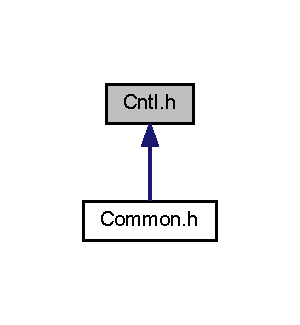
\includegraphics[width=144pt]{_cntl_8h__dep__incl}
\end{center}
\end{figure}
\subsection*{Macros}
\begin{DoxyCompactItemize}
\item 
\#define \hyperlink{_cntl_8h_a64fd24fd8ffc66895ab057370d1c10f9}{S\-A\-T\-M\-A\-X\-\_\-\-M\-A\-X}~0.\-9f
\end{DoxyCompactItemize}
\subsection*{Typedefs}
\begin{DoxyCompactItemize}
\item 
typedef enum \hyperlink{_cntl_8h_a4b8f446b389413b175ff4d4dbcd18da1}{coef\-Num} \hyperlink{_cntl_8h_ac340fbbc5919954c173757935549588f}{cf\-Type}
\end{DoxyCompactItemize}
\subsection*{Enumerations}
\begin{DoxyCompactItemize}
\item 
enum \hyperlink{_cntl_8h_a4b8f446b389413b175ff4d4dbcd18da1}{coef\-Num} \{ , \\*
\hyperlink{_cntl_8h_a4b8f446b389413b175ff4d4dbcd18da1ad15b967851188a21b2d4fd326304bf83}{c\-Min} = first\-Coef, 
\hyperlink{_cntl_8h_a4b8f446b389413b175ff4d4dbcd18da1a3576a9eb4b8f9d1ca3d31a0f9b889299}{c\-Max}, 
\hyperlink{_cntl_8h_a4b8f446b389413b175ff4d4dbcd18da1a3dec162fc3f68f49f43775eba612e110}{c\-B0}, 
\hyperlink{_cntl_8h_a4b8f446b389413b175ff4d4dbcd18da1a43986b141584b760c8c8c9fc29304de2}{c\-B1}, 
\\*
\hyperlink{_cntl_8h_a4b8f446b389413b175ff4d4dbcd18da1aac28a7344b33c5e968a79fc27078da99}{c\-A1}, 
\hyperlink{_cntl_8h_a4b8f446b389413b175ff4d4dbcd18da1a5229cb73bab727c5aeaae425a4fd2472}{c\-B2}, 
\hyperlink{_cntl_8h_a4b8f446b389413b175ff4d4dbcd18da1a80d8d6d72b42fa8603b71cba71e13ef2}{c\-A2}, 
\hyperlink{_cntl_8h_a4b8f446b389413b175ff4d4dbcd18da1aaf02fe4d8a1a90d96d8ceb29c6face14}{c\-B3}, 
\\*
\hyperlink{_cntl_8h_a4b8f446b389413b175ff4d4dbcd18da1a23a7967c17fd0f99330009d84750ff62}{c\-A3}
 \}
\end{DoxyCompactItemize}
\subsection*{Functions}
\begin{DoxyCompactItemize}
\item 
void \hyperlink{_cntl_8h_ac82b19f3b880ae3bbed395b3194d709e}{cntl\-Update\-Coefs} (void)
\item 
Uint16 \hyperlink{_cntl_8h_abc7c9f468b60d7348e835e6473a34b23}{cntl\-Get\-Coef} (Uint16 chnl, \hyperlink{_cntl_8h_ac340fbbc5919954c173757935549588f}{cf\-Type} coef, float32 $\ast$val\-Dest)
\item 
Uint16 \hyperlink{_cntl_8h_a1b0f822cb4344a66c433d36c8eee2be3}{cntl\-Set\-Coef} (Uint16 chnl, \hyperlink{_cntl_8h_ac340fbbc5919954c173757935549588f}{cf\-Type} coef, float32 val)
\end{DoxyCompactItemize}
\subsection*{Variables}
\begin{DoxyCompactItemize}
\item 
volatile int32 $\ast$ \hyperlink{_cntl_8h_a047c759a71b80d8cfd5e6f52b1b021b9}{C\-N\-T\-L\-\_\-2\-P2\-Z\-\_\-\-Coef1}
\item 
volatile int32 $\ast$ \hyperlink{_cntl_8h_abdc599cbabc62898c49926678c3327e6}{C\-N\-T\-L\-\_\-2\-P2\-Z\-\_\-\-Coef2}
\item 
volatile int32 $\ast$ \hyperlink{_cntl_8h_a1e357d296e76299ea04d7a63e4c46d1b}{C\-N\-T\-L\-\_\-2\-P2\-Z\-\_\-\-Coef3}
\item 
volatile int32 $\ast$ \hyperlink{_cntl_8h_afe468cb1e995b267671e88b8d292aef6}{C\-N\-T\-L\-\_\-2\-P2\-Z\-\_\-\-Coef4}
\item 
volatile int32 $\ast$ \hyperlink{_cntl_8h_a5fe3f4dd6aac27512c9e0b6fc843b0b6}{C\-N\-T\-L\-\_\-2\-P2\-Z\-\_\-\-Coef5}
\item 
volatile int32 $\ast$ \hyperlink{_cntl_8h_a9c0418a780375035750c3d4dc16f3ae4}{C\-N\-T\-L\-\_\-2\-P2\-Z\-\_\-\-Fdbk1}
\item 
volatile int32 $\ast$ \hyperlink{_cntl_8h_a6092ef1c1c54802bb5e11564f782390d}{C\-N\-T\-L\-\_\-2\-P2\-Z\-\_\-\-Fdbk2}
\item 
volatile int32 $\ast$ \hyperlink{_cntl_8h_a939782d23ddbf7f45e5e393a65bafcff}{C\-N\-T\-L\-\_\-2\-P2\-Z\-\_\-\-Fdbk3}
\item 
volatile int32 $\ast$ \hyperlink{_cntl_8h_a6937e965f3ae840ea6ee43cce410680f}{C\-N\-T\-L\-\_\-2\-P2\-Z\-\_\-\-Fdbk4}
\item 
volatile int32 $\ast$ \hyperlink{_cntl_8h_af5cbb635f31bbebd041e8543deb40dee}{C\-N\-T\-L\-\_\-2\-P2\-Z\-\_\-\-Fdbk5}
\item 
volatile int32 $\ast$ \hyperlink{_cntl_8h_a84d7c096ca668d1edc5e4fa54abe5d98}{C\-N\-T\-L\-\_\-2\-P2\-Z\-\_\-\-Out1}
\item 
volatile int32 $\ast$ \hyperlink{_cntl_8h_ae6679b66ffeca93742f973a2c947855f}{C\-N\-T\-L\-\_\-2\-P2\-Z\-\_\-\-Out2}
\item 
volatile int32 $\ast$ \hyperlink{_cntl_8h_a11dcb9f6b6d03fe960ddf790e1ad5ed2}{C\-N\-T\-L\-\_\-2\-P2\-Z\-\_\-\-Out3}
\item 
volatile int32 $\ast$ \hyperlink{_cntl_8h_a253e4070b19470606e0566ff25fc911f}{C\-N\-T\-L\-\_\-2\-P2\-Z\-\_\-\-Out4}
\item 
volatile int32 $\ast$ \hyperlink{_cntl_8h_a3b336a91d25a7feb9f8927b32b800d0d}{C\-N\-T\-L\-\_\-2\-P2\-Z\-\_\-\-Out5}
\item 
volatile int32 $\ast$ \hyperlink{_cntl_8h_a98527ce76f5175fa2933d46f324d85fb}{C\-N\-T\-L\-\_\-2\-P2\-Z\-\_\-\-Ref1}
\item 
volatile int32 $\ast$ \hyperlink{_cntl_8h_a9bf1756a901a3a74d9f43a51f85cede4}{C\-N\-T\-L\-\_\-2\-P2\-Z\-\_\-\-Ref2}
\item 
volatile int32 $\ast$ \hyperlink{_cntl_8h_a859e9bbd5bc82f1b42863a93e4f992af}{C\-N\-T\-L\-\_\-2\-P2\-Z\-\_\-\-Ref3}
\item 
volatile int32 $\ast$ \hyperlink{_cntl_8h_af54c55f228deb8189c44282a94a870c1}{C\-N\-T\-L\-\_\-2\-P2\-Z\-\_\-\-Ref4}
\item 
volatile int32 $\ast$ \hyperlink{_cntl_8h_abd3b240e2d3f7d3f4f717066ee8efd3e}{C\-N\-T\-L\-\_\-2\-P2\-Z\-\_\-\-Ref5}
\item 
volatile int32 $\ast$ \hyperlink{_cntl_8h_a41005c53e7c439f0af28e140f7d3d0ed}{C\-N\-T\-L\-\_\-3\-P3\-Z\-\_\-\-Coef1}
\item 
volatile int32 $\ast$ \hyperlink{_cntl_8h_a7a74642d86ae9a823f58f49db57f8bc8}{C\-N\-T\-L\-\_\-3\-P3\-Z\-\_\-\-Coef2}
\item 
volatile int32 $\ast$ \hyperlink{_cntl_8h_a361372a23d9146cd2d077e6c843ec47e}{C\-N\-T\-L\-\_\-3\-P3\-Z\-\_\-\-Fdbk1}
\item 
volatile int32 $\ast$ \hyperlink{_cntl_8h_a4676fa58f77cab7e1c4e86255049dfe7}{C\-N\-T\-L\-\_\-3\-P3\-Z\-\_\-\-Fdbk2}
\item 
volatile int32 $\ast$ \hyperlink{_cntl_8h_acb0edbb1cfd2fb0e63ac2eb233dcd577}{C\-N\-T\-L\-\_\-3\-P3\-Z\-\_\-\-Out1}
\item 
volatile int32 $\ast$ \hyperlink{_cntl_8h_a92dd8eabeed10eaaaf60887d9bcbd76d}{C\-N\-T\-L\-\_\-3\-P3\-Z\-\_\-\-Out2}
\item 
volatile int32 $\ast$ \hyperlink{_cntl_8h_a6ebe91dab023eff56cade0eddcd3e96d}{C\-N\-T\-L\-\_\-3\-P3\-Z\-\_\-\-Ref1}
\item 
volatile int32 $\ast$ \hyperlink{_cntl_8h_a589e93bad0b8ba223e32ce590bba816b}{C\-N\-T\-L\-\_\-3\-P3\-Z\-\_\-\-Ref2}
\item 
struct C\-N\-T\-L\-\_\-2\-P2\-Z\-\_\-\-Coef\-Struct \hyperlink{_cntl_8h_a0e862b208ff3b2bb45fcfce1ccd74cd2}{coefs2} \mbox{[}\hyperlink{_settings_8h_a69b2e41c3deaae85991311202c4a1a14}{N\-U\-M\-\_\-\-I\-C\-T\-R\-L\-\_\-\-C\-H\-N\-L\-S}\mbox{]}
\item 
struct C\-N\-T\-L\-\_\-3\-P3\-Z\-\_\-\-Coef\-Struct \hyperlink{_cntl_8h_a84b8a9f9bc8749e7ad42eea593f858c4}{coefs3} \mbox{[}\hyperlink{_settings_8h_a42a316162edffd07a32e68a889760c06}{N\-U\-M\-\_\-\-V\-C\-T\-R\-L\-\_\-\-C\-H\-N\-L\-S}\mbox{]}
\end{DoxyCompactItemize}


\subsection{Detailed Description}
D\-P\-Lib C\-N\-T\-L Macro related helper functions. 

\subsection{Macro Definition Documentation}
\hypertarget{_cntl_8h_a64fd24fd8ffc66895ab057370d1c10f9}{\index{Cntl.\-h@{Cntl.\-h}!S\-A\-T\-M\-A\-X\-\_\-\-M\-A\-X@{S\-A\-T\-M\-A\-X\-\_\-\-M\-A\-X}}
\index{S\-A\-T\-M\-A\-X\-\_\-\-M\-A\-X@{S\-A\-T\-M\-A\-X\-\_\-\-M\-A\-X}!Cntl.h@{Cntl.\-h}}
\subsubsection[{S\-A\-T\-M\-A\-X\-\_\-\-M\-A\-X}]{\setlength{\rightskip}{0pt plus 5cm}\#define S\-A\-T\-M\-A\-X\-\_\-\-M\-A\-X~0.\-9f}}\label{_cntl_8h_a64fd24fd8ffc66895ab057370d1c10f9}
The maximum allowable value for the I\-I\-R filter control law's maximum saturation. 

\subsection{Typedef Documentation}
\hypertarget{_cntl_8h_ac340fbbc5919954c173757935549588f}{\index{Cntl.\-h@{Cntl.\-h}!cf\-Type@{cf\-Type}}
\index{cf\-Type@{cf\-Type}!Cntl.h@{Cntl.\-h}}
\subsubsection[{cf\-Type}]{\setlength{\rightskip}{0pt plus 5cm}typedef enum {\bf coef\-Num} {\bf cf\-Type}}}\label{_cntl_8h_ac340fbbc5919954c173757935549588f}
A type that allows a reference to a C\-N\-T\-L coefficient. 

\subsection{Enumeration Type Documentation}
\hypertarget{_cntl_8h_a4b8f446b389413b175ff4d4dbcd18da1}{\index{Cntl.\-h@{Cntl.\-h}!coef\-Num@{coef\-Num}}
\index{coef\-Num@{coef\-Num}!Cntl.h@{Cntl.\-h}}
\subsubsection[{coef\-Num}]{\setlength{\rightskip}{0pt plus 5cm}enum {\bf coef\-Num}}}\label{_cntl_8h_a4b8f446b389413b175ff4d4dbcd18da1}
C\-N\-T\-L Coefficient references \begin{Desc}
\item[Enumerator]\par
\begin{description}
\index{c\-Min@{c\-Min}!Cntl.\-h@{Cntl.\-h}}\index{Cntl.\-h@{Cntl.\-h}!c\-Min@{c\-Min}}\item[{\em 
\hypertarget{_cntl_8h_a4b8f446b389413b175ff4d4dbcd18da1ad15b967851188a21b2d4fd326304bf83}{c\-Min}\label{_cntl_8h_a4b8f446b389413b175ff4d4dbcd18da1ad15b967851188a21b2d4fd326304bf83}
}]Saturation minimum reference. \index{c\-Max@{c\-Max}!Cntl.\-h@{Cntl.\-h}}\index{Cntl.\-h@{Cntl.\-h}!c\-Max@{c\-Max}}\item[{\em 
\hypertarget{_cntl_8h_a4b8f446b389413b175ff4d4dbcd18da1a3576a9eb4b8f9d1ca3d31a0f9b889299}{c\-Max}\label{_cntl_8h_a4b8f446b389413b175ff4d4dbcd18da1a3576a9eb4b8f9d1ca3d31a0f9b889299}
}]Saturation maximum reference. \index{c\-B0@{c\-B0}!Cntl.\-h@{Cntl.\-h}}\index{Cntl.\-h@{Cntl.\-h}!c\-B0@{c\-B0}}\item[{\em 
\hypertarget{_cntl_8h_a4b8f446b389413b175ff4d4dbcd18da1a3dec162fc3f68f49f43775eba612e110}{c\-B0}\label{_cntl_8h_a4b8f446b389413b175ff4d4dbcd18da1a3dec162fc3f68f49f43775eba612e110}
}]B0 coefficient reference. \index{c\-B1@{c\-B1}!Cntl.\-h@{Cntl.\-h}}\index{Cntl.\-h@{Cntl.\-h}!c\-B1@{c\-B1}}\item[{\em 
\hypertarget{_cntl_8h_a4b8f446b389413b175ff4d4dbcd18da1a43986b141584b760c8c8c9fc29304de2}{c\-B1}\label{_cntl_8h_a4b8f446b389413b175ff4d4dbcd18da1a43986b141584b760c8c8c9fc29304de2}
}]B1 coefficient reference. \index{c\-A1@{c\-A1}!Cntl.\-h@{Cntl.\-h}}\index{Cntl.\-h@{Cntl.\-h}!c\-A1@{c\-A1}}\item[{\em 
\hypertarget{_cntl_8h_a4b8f446b389413b175ff4d4dbcd18da1aac28a7344b33c5e968a79fc27078da99}{c\-A1}\label{_cntl_8h_a4b8f446b389413b175ff4d4dbcd18da1aac28a7344b33c5e968a79fc27078da99}
}]A1 coefficient reference. \index{c\-B2@{c\-B2}!Cntl.\-h@{Cntl.\-h}}\index{Cntl.\-h@{Cntl.\-h}!c\-B2@{c\-B2}}\item[{\em 
\hypertarget{_cntl_8h_a4b8f446b389413b175ff4d4dbcd18da1a5229cb73bab727c5aeaae425a4fd2472}{c\-B2}\label{_cntl_8h_a4b8f446b389413b175ff4d4dbcd18da1a5229cb73bab727c5aeaae425a4fd2472}
}]B2 coefficient reference. \index{c\-A2@{c\-A2}!Cntl.\-h@{Cntl.\-h}}\index{Cntl.\-h@{Cntl.\-h}!c\-A2@{c\-A2}}\item[{\em 
\hypertarget{_cntl_8h_a4b8f446b389413b175ff4d4dbcd18da1a80d8d6d72b42fa8603b71cba71e13ef2}{c\-A2}\label{_cntl_8h_a4b8f446b389413b175ff4d4dbcd18da1a80d8d6d72b42fa8603b71cba71e13ef2}
}]A2 coefficient reference. \index{c\-B3@{c\-B3}!Cntl.\-h@{Cntl.\-h}}\index{Cntl.\-h@{Cntl.\-h}!c\-B3@{c\-B3}}\item[{\em 
\hypertarget{_cntl_8h_a4b8f446b389413b175ff4d4dbcd18da1aaf02fe4d8a1a90d96d8ceb29c6face14}{c\-B3}\label{_cntl_8h_a4b8f446b389413b175ff4d4dbcd18da1aaf02fe4d8a1a90d96d8ceb29c6face14}
}]B3 coefficient reference. \index{c\-A3@{c\-A3}!Cntl.\-h@{Cntl.\-h}}\index{Cntl.\-h@{Cntl.\-h}!c\-A3@{c\-A3}}\item[{\em 
\hypertarget{_cntl_8h_a4b8f446b389413b175ff4d4dbcd18da1a23a7967c17fd0f99330009d84750ff62}{c\-A3}\label{_cntl_8h_a4b8f446b389413b175ff4d4dbcd18da1a23a7967c17fd0f99330009d84750ff62}
}]A3 coefficient reference. \end{description}
\end{Desc}


\subsection{Function Documentation}
\hypertarget{_cntl_8h_abc7c9f468b60d7348e835e6473a34b23}{\index{Cntl.\-h@{Cntl.\-h}!cntl\-Get\-Coef@{cntl\-Get\-Coef}}
\index{cntl\-Get\-Coef@{cntl\-Get\-Coef}!Cntl.h@{Cntl.\-h}}
\subsubsection[{cntl\-Get\-Coef}]{\setlength{\rightskip}{0pt plus 5cm}Uint16 cntl\-Get\-Coef (
\begin{DoxyParamCaption}
\item[{Uint16}]{chnl, }
\item[{{\bf cf\-Type}}]{coef, }
\item[{float32 $\ast$}]{val\-Dest}
\end{DoxyParamCaption}
)}}\label{_cntl_8h_abc7c9f468b60d7348e835e6473a34b23}
Queries the specified I\-I\-R filter control law coefficient for the specified channel. 
\begin{DoxyParams}[1]{Parameters}
\mbox{\tt in}  & {\em chnl} & Specifies the channel number on which the setting is to be queried. \\
\hline
\mbox{\tt in}  & {\em coef} & Specifies the coefficient to be queried. \\
\hline
\mbox{\tt out}  & {\em val\-Dest} & Address of the memory location at which to place the query result. \\
\hline
\end{DoxyParams}
\begin{DoxyReturn}{Returns}
Error status. 
\end{DoxyReturn}
\hypertarget{_cntl_8h_a1b0f822cb4344a66c433d36c8eee2be3}{\index{Cntl.\-h@{Cntl.\-h}!cntl\-Set\-Coef@{cntl\-Set\-Coef}}
\index{cntl\-Set\-Coef@{cntl\-Set\-Coef}!Cntl.h@{Cntl.\-h}}
\subsubsection[{cntl\-Set\-Coef}]{\setlength{\rightskip}{0pt plus 5cm}Uint16 cntl\-Set\-Coef (
\begin{DoxyParamCaption}
\item[{Uint16}]{chnl, }
\item[{{\bf cf\-Type}}]{coef, }
\item[{float32}]{val}
\end{DoxyParamCaption}
)}}\label{_cntl_8h_a1b0f822cb4344a66c433d36c8eee2be3}
Sets the specified I\-I\-R filter control law coefficient for the specified channel.
\begin{DoxyItemize}
\item The actual setting in use is not updated until A\-F\-T\-E\-R \hyperlink{_cntl_8h_ac82b19f3b880ae3bbed395b3194d709e}{cntl\-Update\-Coefs()} has been called. 
\begin{DoxyParams}[1]{Parameters}
\mbox{\tt in}  & {\em chnl} & Specifies the channel number the setting is to be applied to \mbox{[}0, N\-U\-M\-\_\-\-C\-H\-N\-L\-S). \\
\hline
\mbox{\tt in}  & {\em coef} & Specifies the coefficient to be set \mbox{[}c\-Min, c\-A3). \\
\hline
\mbox{\tt in}  & {\em val} & Specifies the coefficient value to be applied. Should be between the minimum and maximum values for the specific coefficient as defined by cf\-Lmts\mbox{[}coef\mbox{]} and cf\-Lmts\mbox{[}coef + c\-A3\mbox{]}. \\
\hline
\end{DoxyParams}
\begin{DoxyReturn}{Returns}
Error status. 
\end{DoxyReturn}

\end{DoxyItemize}\hypertarget{_cntl_8h_ac82b19f3b880ae3bbed395b3194d709e}{\index{Cntl.\-h@{Cntl.\-h}!cntl\-Update\-Coefs@{cntl\-Update\-Coefs}}
\index{cntl\-Update\-Coefs@{cntl\-Update\-Coefs}!Cntl.h@{Cntl.\-h}}
\subsubsection[{cntl\-Update\-Coefs}]{\setlength{\rightskip}{0pt plus 5cm}void cntl\-Update\-Coefs (
\begin{DoxyParamCaption}
\item[{void}]{}
\end{DoxyParamCaption}
)}}\label{_cntl_8h_ac82b19f3b880ae3bbed395b3194d709e}
Updates the I\-I\-R filter control law's coefficients that are being used to those values set by the use of the other functions within this file. 

\subsection{Variable Documentation}
\hypertarget{_cntl_8h_a047c759a71b80d8cfd5e6f52b1b021b9}{\index{Cntl.\-h@{Cntl.\-h}!C\-N\-T\-L\-\_\-2\-P2\-Z\-\_\-\-Coef1@{C\-N\-T\-L\-\_\-2\-P2\-Z\-\_\-\-Coef1}}
\index{C\-N\-T\-L\-\_\-2\-P2\-Z\-\_\-\-Coef1@{C\-N\-T\-L\-\_\-2\-P2\-Z\-\_\-\-Coef1}!Cntl.h@{Cntl.\-h}}
\subsubsection[{C\-N\-T\-L\-\_\-2\-P2\-Z\-\_\-\-Coef1}]{\setlength{\rightskip}{0pt plus 5cm}volatile int32$\ast$ C\-N\-T\-L\-\_\-2\-P2\-Z\-\_\-\-Coef1}}\label{_cntl_8h_a047c759a71b80d8cfd5e6f52b1b021b9}
Channel 0 I\-I\-R filter control law coefficient terminal pointer. \hypertarget{_cntl_8h_abdc599cbabc62898c49926678c3327e6}{\index{Cntl.\-h@{Cntl.\-h}!C\-N\-T\-L\-\_\-2\-P2\-Z\-\_\-\-Coef2@{C\-N\-T\-L\-\_\-2\-P2\-Z\-\_\-\-Coef2}}
\index{C\-N\-T\-L\-\_\-2\-P2\-Z\-\_\-\-Coef2@{C\-N\-T\-L\-\_\-2\-P2\-Z\-\_\-\-Coef2}!Cntl.h@{Cntl.\-h}}
\subsubsection[{C\-N\-T\-L\-\_\-2\-P2\-Z\-\_\-\-Coef2}]{\setlength{\rightskip}{0pt plus 5cm}volatile int32$\ast$ C\-N\-T\-L\-\_\-2\-P2\-Z\-\_\-\-Coef2}}\label{_cntl_8h_abdc599cbabc62898c49926678c3327e6}
Channel 1 I\-I\-R filter control law coefficient terminal pointer. \hypertarget{_cntl_8h_a1e357d296e76299ea04d7a63e4c46d1b}{\index{Cntl.\-h@{Cntl.\-h}!C\-N\-T\-L\-\_\-2\-P2\-Z\-\_\-\-Coef3@{C\-N\-T\-L\-\_\-2\-P2\-Z\-\_\-\-Coef3}}
\index{C\-N\-T\-L\-\_\-2\-P2\-Z\-\_\-\-Coef3@{C\-N\-T\-L\-\_\-2\-P2\-Z\-\_\-\-Coef3}!Cntl.h@{Cntl.\-h}}
\subsubsection[{C\-N\-T\-L\-\_\-2\-P2\-Z\-\_\-\-Coef3}]{\setlength{\rightskip}{0pt plus 5cm}volatile int32$\ast$ C\-N\-T\-L\-\_\-2\-P2\-Z\-\_\-\-Coef3}}\label{_cntl_8h_a1e357d296e76299ea04d7a63e4c46d1b}
Channel 2 I\-I\-R filter control law coefficient terminal pointer. \hypertarget{_cntl_8h_afe468cb1e995b267671e88b8d292aef6}{\index{Cntl.\-h@{Cntl.\-h}!C\-N\-T\-L\-\_\-2\-P2\-Z\-\_\-\-Coef4@{C\-N\-T\-L\-\_\-2\-P2\-Z\-\_\-\-Coef4}}
\index{C\-N\-T\-L\-\_\-2\-P2\-Z\-\_\-\-Coef4@{C\-N\-T\-L\-\_\-2\-P2\-Z\-\_\-\-Coef4}!Cntl.h@{Cntl.\-h}}
\subsubsection[{C\-N\-T\-L\-\_\-2\-P2\-Z\-\_\-\-Coef4}]{\setlength{\rightskip}{0pt plus 5cm}volatile int32$\ast$ C\-N\-T\-L\-\_\-2\-P2\-Z\-\_\-\-Coef4}}\label{_cntl_8h_afe468cb1e995b267671e88b8d292aef6}
Channel 3 I\-I\-R filter control law coefficient terminal pointer. \hypertarget{_cntl_8h_a5fe3f4dd6aac27512c9e0b6fc843b0b6}{\index{Cntl.\-h@{Cntl.\-h}!C\-N\-T\-L\-\_\-2\-P2\-Z\-\_\-\-Coef5@{C\-N\-T\-L\-\_\-2\-P2\-Z\-\_\-\-Coef5}}
\index{C\-N\-T\-L\-\_\-2\-P2\-Z\-\_\-\-Coef5@{C\-N\-T\-L\-\_\-2\-P2\-Z\-\_\-\-Coef5}!Cntl.h@{Cntl.\-h}}
\subsubsection[{C\-N\-T\-L\-\_\-2\-P2\-Z\-\_\-\-Coef5}]{\setlength{\rightskip}{0pt plus 5cm}volatile int32$\ast$ C\-N\-T\-L\-\_\-2\-P2\-Z\-\_\-\-Coef5}}\label{_cntl_8h_a5fe3f4dd6aac27512c9e0b6fc843b0b6}
Channel 4 I\-I\-R filter control law coefficient terminal pointer. \hypertarget{_cntl_8h_a9c0418a780375035750c3d4dc16f3ae4}{\index{Cntl.\-h@{Cntl.\-h}!C\-N\-T\-L\-\_\-2\-P2\-Z\-\_\-\-Fdbk1@{C\-N\-T\-L\-\_\-2\-P2\-Z\-\_\-\-Fdbk1}}
\index{C\-N\-T\-L\-\_\-2\-P2\-Z\-\_\-\-Fdbk1@{C\-N\-T\-L\-\_\-2\-P2\-Z\-\_\-\-Fdbk1}!Cntl.h@{Cntl.\-h}}
\subsubsection[{C\-N\-T\-L\-\_\-2\-P2\-Z\-\_\-\-Fdbk1}]{\setlength{\rightskip}{0pt plus 5cm}volatile int32$\ast$ C\-N\-T\-L\-\_\-2\-P2\-Z\-\_\-\-Fdbk1}}\label{_cntl_8h_a9c0418a780375035750c3d4dc16f3ae4}
Channel 0 I\-I\-R filter control law feedback terminal pointer. \hypertarget{_cntl_8h_a6092ef1c1c54802bb5e11564f782390d}{\index{Cntl.\-h@{Cntl.\-h}!C\-N\-T\-L\-\_\-2\-P2\-Z\-\_\-\-Fdbk2@{C\-N\-T\-L\-\_\-2\-P2\-Z\-\_\-\-Fdbk2}}
\index{C\-N\-T\-L\-\_\-2\-P2\-Z\-\_\-\-Fdbk2@{C\-N\-T\-L\-\_\-2\-P2\-Z\-\_\-\-Fdbk2}!Cntl.h@{Cntl.\-h}}
\subsubsection[{C\-N\-T\-L\-\_\-2\-P2\-Z\-\_\-\-Fdbk2}]{\setlength{\rightskip}{0pt plus 5cm}volatile int32$\ast$ C\-N\-T\-L\-\_\-2\-P2\-Z\-\_\-\-Fdbk2}}\label{_cntl_8h_a6092ef1c1c54802bb5e11564f782390d}
Channel 1 I\-I\-R filter control law feedback terminal pointer. \hypertarget{_cntl_8h_a939782d23ddbf7f45e5e393a65bafcff}{\index{Cntl.\-h@{Cntl.\-h}!C\-N\-T\-L\-\_\-2\-P2\-Z\-\_\-\-Fdbk3@{C\-N\-T\-L\-\_\-2\-P2\-Z\-\_\-\-Fdbk3}}
\index{C\-N\-T\-L\-\_\-2\-P2\-Z\-\_\-\-Fdbk3@{C\-N\-T\-L\-\_\-2\-P2\-Z\-\_\-\-Fdbk3}!Cntl.h@{Cntl.\-h}}
\subsubsection[{C\-N\-T\-L\-\_\-2\-P2\-Z\-\_\-\-Fdbk3}]{\setlength{\rightskip}{0pt plus 5cm}volatile int32$\ast$ C\-N\-T\-L\-\_\-2\-P2\-Z\-\_\-\-Fdbk3}}\label{_cntl_8h_a939782d23ddbf7f45e5e393a65bafcff}
Channel 2 I\-I\-R filter control law feedback terminal pointer. \hypertarget{_cntl_8h_a6937e965f3ae840ea6ee43cce410680f}{\index{Cntl.\-h@{Cntl.\-h}!C\-N\-T\-L\-\_\-2\-P2\-Z\-\_\-\-Fdbk4@{C\-N\-T\-L\-\_\-2\-P2\-Z\-\_\-\-Fdbk4}}
\index{C\-N\-T\-L\-\_\-2\-P2\-Z\-\_\-\-Fdbk4@{C\-N\-T\-L\-\_\-2\-P2\-Z\-\_\-\-Fdbk4}!Cntl.h@{Cntl.\-h}}
\subsubsection[{C\-N\-T\-L\-\_\-2\-P2\-Z\-\_\-\-Fdbk4}]{\setlength{\rightskip}{0pt plus 5cm}volatile int32$\ast$ C\-N\-T\-L\-\_\-2\-P2\-Z\-\_\-\-Fdbk4}}\label{_cntl_8h_a6937e965f3ae840ea6ee43cce410680f}
Channel 3 I\-I\-R filter control law feedback terminal pointer. \hypertarget{_cntl_8h_af5cbb635f31bbebd041e8543deb40dee}{\index{Cntl.\-h@{Cntl.\-h}!C\-N\-T\-L\-\_\-2\-P2\-Z\-\_\-\-Fdbk5@{C\-N\-T\-L\-\_\-2\-P2\-Z\-\_\-\-Fdbk5}}
\index{C\-N\-T\-L\-\_\-2\-P2\-Z\-\_\-\-Fdbk5@{C\-N\-T\-L\-\_\-2\-P2\-Z\-\_\-\-Fdbk5}!Cntl.h@{Cntl.\-h}}
\subsubsection[{C\-N\-T\-L\-\_\-2\-P2\-Z\-\_\-\-Fdbk5}]{\setlength{\rightskip}{0pt plus 5cm}volatile int32$\ast$ C\-N\-T\-L\-\_\-2\-P2\-Z\-\_\-\-Fdbk5}}\label{_cntl_8h_af5cbb635f31bbebd041e8543deb40dee}
Channel 4 I\-I\-R filter control law feedback terminal pointer. \hypertarget{_cntl_8h_a84d7c096ca668d1edc5e4fa54abe5d98}{\index{Cntl.\-h@{Cntl.\-h}!C\-N\-T\-L\-\_\-2\-P2\-Z\-\_\-\-Out1@{C\-N\-T\-L\-\_\-2\-P2\-Z\-\_\-\-Out1}}
\index{C\-N\-T\-L\-\_\-2\-P2\-Z\-\_\-\-Out1@{C\-N\-T\-L\-\_\-2\-P2\-Z\-\_\-\-Out1}!Cntl.h@{Cntl.\-h}}
\subsubsection[{C\-N\-T\-L\-\_\-2\-P2\-Z\-\_\-\-Out1}]{\setlength{\rightskip}{0pt plus 5cm}volatile int32$\ast$ C\-N\-T\-L\-\_\-2\-P2\-Z\-\_\-\-Out1}}\label{_cntl_8h_a84d7c096ca668d1edc5e4fa54abe5d98}
Channel 0 I\-I\-R filter control law output terminal pointer. \hypertarget{_cntl_8h_ae6679b66ffeca93742f973a2c947855f}{\index{Cntl.\-h@{Cntl.\-h}!C\-N\-T\-L\-\_\-2\-P2\-Z\-\_\-\-Out2@{C\-N\-T\-L\-\_\-2\-P2\-Z\-\_\-\-Out2}}
\index{C\-N\-T\-L\-\_\-2\-P2\-Z\-\_\-\-Out2@{C\-N\-T\-L\-\_\-2\-P2\-Z\-\_\-\-Out2}!Cntl.h@{Cntl.\-h}}
\subsubsection[{C\-N\-T\-L\-\_\-2\-P2\-Z\-\_\-\-Out2}]{\setlength{\rightskip}{0pt plus 5cm}volatile int32$\ast$ C\-N\-T\-L\-\_\-2\-P2\-Z\-\_\-\-Out2}}\label{_cntl_8h_ae6679b66ffeca93742f973a2c947855f}
Channel 1 I\-I\-R filter control law output terminal pointer. \hypertarget{_cntl_8h_a11dcb9f6b6d03fe960ddf790e1ad5ed2}{\index{Cntl.\-h@{Cntl.\-h}!C\-N\-T\-L\-\_\-2\-P2\-Z\-\_\-\-Out3@{C\-N\-T\-L\-\_\-2\-P2\-Z\-\_\-\-Out3}}
\index{C\-N\-T\-L\-\_\-2\-P2\-Z\-\_\-\-Out3@{C\-N\-T\-L\-\_\-2\-P2\-Z\-\_\-\-Out3}!Cntl.h@{Cntl.\-h}}
\subsubsection[{C\-N\-T\-L\-\_\-2\-P2\-Z\-\_\-\-Out3}]{\setlength{\rightskip}{0pt plus 5cm}volatile int32$\ast$ C\-N\-T\-L\-\_\-2\-P2\-Z\-\_\-\-Out3}}\label{_cntl_8h_a11dcb9f6b6d03fe960ddf790e1ad5ed2}
Channel 2 I\-I\-R filter control law output terminal pointer. \hypertarget{_cntl_8h_a253e4070b19470606e0566ff25fc911f}{\index{Cntl.\-h@{Cntl.\-h}!C\-N\-T\-L\-\_\-2\-P2\-Z\-\_\-\-Out4@{C\-N\-T\-L\-\_\-2\-P2\-Z\-\_\-\-Out4}}
\index{C\-N\-T\-L\-\_\-2\-P2\-Z\-\_\-\-Out4@{C\-N\-T\-L\-\_\-2\-P2\-Z\-\_\-\-Out4}!Cntl.h@{Cntl.\-h}}
\subsubsection[{C\-N\-T\-L\-\_\-2\-P2\-Z\-\_\-\-Out4}]{\setlength{\rightskip}{0pt plus 5cm}volatile int32$\ast$ C\-N\-T\-L\-\_\-2\-P2\-Z\-\_\-\-Out4}}\label{_cntl_8h_a253e4070b19470606e0566ff25fc911f}
Channel 3 I\-I\-R filter control law output terminal pointer. \hypertarget{_cntl_8h_a3b336a91d25a7feb9f8927b32b800d0d}{\index{Cntl.\-h@{Cntl.\-h}!C\-N\-T\-L\-\_\-2\-P2\-Z\-\_\-\-Out5@{C\-N\-T\-L\-\_\-2\-P2\-Z\-\_\-\-Out5}}
\index{C\-N\-T\-L\-\_\-2\-P2\-Z\-\_\-\-Out5@{C\-N\-T\-L\-\_\-2\-P2\-Z\-\_\-\-Out5}!Cntl.h@{Cntl.\-h}}
\subsubsection[{C\-N\-T\-L\-\_\-2\-P2\-Z\-\_\-\-Out5}]{\setlength{\rightskip}{0pt plus 5cm}volatile int32$\ast$ C\-N\-T\-L\-\_\-2\-P2\-Z\-\_\-\-Out5}}\label{_cntl_8h_a3b336a91d25a7feb9f8927b32b800d0d}
Channel 4 I\-I\-R filter control law output terminal pointer. \hypertarget{_cntl_8h_a98527ce76f5175fa2933d46f324d85fb}{\index{Cntl.\-h@{Cntl.\-h}!C\-N\-T\-L\-\_\-2\-P2\-Z\-\_\-\-Ref1@{C\-N\-T\-L\-\_\-2\-P2\-Z\-\_\-\-Ref1}}
\index{C\-N\-T\-L\-\_\-2\-P2\-Z\-\_\-\-Ref1@{C\-N\-T\-L\-\_\-2\-P2\-Z\-\_\-\-Ref1}!Cntl.h@{Cntl.\-h}}
\subsubsection[{C\-N\-T\-L\-\_\-2\-P2\-Z\-\_\-\-Ref1}]{\setlength{\rightskip}{0pt plus 5cm}volatile int32$\ast$ C\-N\-T\-L\-\_\-2\-P2\-Z\-\_\-\-Ref1}}\label{_cntl_8h_a98527ce76f5175fa2933d46f324d85fb}
Channel 0 I\-I\-R filter control law reference terminal pointer. \hypertarget{_cntl_8h_a9bf1756a901a3a74d9f43a51f85cede4}{\index{Cntl.\-h@{Cntl.\-h}!C\-N\-T\-L\-\_\-2\-P2\-Z\-\_\-\-Ref2@{C\-N\-T\-L\-\_\-2\-P2\-Z\-\_\-\-Ref2}}
\index{C\-N\-T\-L\-\_\-2\-P2\-Z\-\_\-\-Ref2@{C\-N\-T\-L\-\_\-2\-P2\-Z\-\_\-\-Ref2}!Cntl.h@{Cntl.\-h}}
\subsubsection[{C\-N\-T\-L\-\_\-2\-P2\-Z\-\_\-\-Ref2}]{\setlength{\rightskip}{0pt plus 5cm}volatile int32$\ast$ C\-N\-T\-L\-\_\-2\-P2\-Z\-\_\-\-Ref2}}\label{_cntl_8h_a9bf1756a901a3a74d9f43a51f85cede4}
Channel 1 I\-I\-R filter control law reference terminal pointer. \hypertarget{_cntl_8h_a859e9bbd5bc82f1b42863a93e4f992af}{\index{Cntl.\-h@{Cntl.\-h}!C\-N\-T\-L\-\_\-2\-P2\-Z\-\_\-\-Ref3@{C\-N\-T\-L\-\_\-2\-P2\-Z\-\_\-\-Ref3}}
\index{C\-N\-T\-L\-\_\-2\-P2\-Z\-\_\-\-Ref3@{C\-N\-T\-L\-\_\-2\-P2\-Z\-\_\-\-Ref3}!Cntl.h@{Cntl.\-h}}
\subsubsection[{C\-N\-T\-L\-\_\-2\-P2\-Z\-\_\-\-Ref3}]{\setlength{\rightskip}{0pt plus 5cm}volatile int32$\ast$ C\-N\-T\-L\-\_\-2\-P2\-Z\-\_\-\-Ref3}}\label{_cntl_8h_a859e9bbd5bc82f1b42863a93e4f992af}
Channel 2 I\-I\-R filter control law reference terminal pointer. \hypertarget{_cntl_8h_af54c55f228deb8189c44282a94a870c1}{\index{Cntl.\-h@{Cntl.\-h}!C\-N\-T\-L\-\_\-2\-P2\-Z\-\_\-\-Ref4@{C\-N\-T\-L\-\_\-2\-P2\-Z\-\_\-\-Ref4}}
\index{C\-N\-T\-L\-\_\-2\-P2\-Z\-\_\-\-Ref4@{C\-N\-T\-L\-\_\-2\-P2\-Z\-\_\-\-Ref4}!Cntl.h@{Cntl.\-h}}
\subsubsection[{C\-N\-T\-L\-\_\-2\-P2\-Z\-\_\-\-Ref4}]{\setlength{\rightskip}{0pt plus 5cm}volatile int32$\ast$ C\-N\-T\-L\-\_\-2\-P2\-Z\-\_\-\-Ref4}}\label{_cntl_8h_af54c55f228deb8189c44282a94a870c1}
Channel 3 I\-I\-R filter control law reference terminal pointer. \hypertarget{_cntl_8h_abd3b240e2d3f7d3f4f717066ee8efd3e}{\index{Cntl.\-h@{Cntl.\-h}!C\-N\-T\-L\-\_\-2\-P2\-Z\-\_\-\-Ref5@{C\-N\-T\-L\-\_\-2\-P2\-Z\-\_\-\-Ref5}}
\index{C\-N\-T\-L\-\_\-2\-P2\-Z\-\_\-\-Ref5@{C\-N\-T\-L\-\_\-2\-P2\-Z\-\_\-\-Ref5}!Cntl.h@{Cntl.\-h}}
\subsubsection[{C\-N\-T\-L\-\_\-2\-P2\-Z\-\_\-\-Ref5}]{\setlength{\rightskip}{0pt plus 5cm}volatile int32$\ast$ C\-N\-T\-L\-\_\-2\-P2\-Z\-\_\-\-Ref5}}\label{_cntl_8h_abd3b240e2d3f7d3f4f717066ee8efd3e}
Channel 4 I\-I\-R filter control law reference terminal pointer. \hypertarget{_cntl_8h_a41005c53e7c439f0af28e140f7d3d0ed}{\index{Cntl.\-h@{Cntl.\-h}!C\-N\-T\-L\-\_\-3\-P3\-Z\-\_\-\-Coef1@{C\-N\-T\-L\-\_\-3\-P3\-Z\-\_\-\-Coef1}}
\index{C\-N\-T\-L\-\_\-3\-P3\-Z\-\_\-\-Coef1@{C\-N\-T\-L\-\_\-3\-P3\-Z\-\_\-\-Coef1}!Cntl.h@{Cntl.\-h}}
\subsubsection[{C\-N\-T\-L\-\_\-3\-P3\-Z\-\_\-\-Coef1}]{\setlength{\rightskip}{0pt plus 5cm}volatile int32$\ast$ C\-N\-T\-L\-\_\-3\-P3\-Z\-\_\-\-Coef1}}\label{_cntl_8h_a41005c53e7c439f0af28e140f7d3d0ed}
Interboost I\-I\-R filter control law coefficient terminal pointer. \hypertarget{_cntl_8h_a7a74642d86ae9a823f58f49db57f8bc8}{\index{Cntl.\-h@{Cntl.\-h}!C\-N\-T\-L\-\_\-3\-P3\-Z\-\_\-\-Coef2@{C\-N\-T\-L\-\_\-3\-P3\-Z\-\_\-\-Coef2}}
\index{C\-N\-T\-L\-\_\-3\-P3\-Z\-\_\-\-Coef2@{C\-N\-T\-L\-\_\-3\-P3\-Z\-\_\-\-Coef2}!Cntl.h@{Cntl.\-h}}
\subsubsection[{C\-N\-T\-L\-\_\-3\-P3\-Z\-\_\-\-Coef2}]{\setlength{\rightskip}{0pt plus 5cm}volatile int32$\ast$ C\-N\-T\-L\-\_\-3\-P3\-Z\-\_\-\-Coef2}}\label{_cntl_8h_a7a74642d86ae9a823f58f49db57f8bc8}
A\-C stage I\-I\-R filter control law coefficient terminal pointer. \hypertarget{_cntl_8h_a361372a23d9146cd2d077e6c843ec47e}{\index{Cntl.\-h@{Cntl.\-h}!C\-N\-T\-L\-\_\-3\-P3\-Z\-\_\-\-Fdbk1@{C\-N\-T\-L\-\_\-3\-P3\-Z\-\_\-\-Fdbk1}}
\index{C\-N\-T\-L\-\_\-3\-P3\-Z\-\_\-\-Fdbk1@{C\-N\-T\-L\-\_\-3\-P3\-Z\-\_\-\-Fdbk1}!Cntl.h@{Cntl.\-h}}
\subsubsection[{C\-N\-T\-L\-\_\-3\-P3\-Z\-\_\-\-Fdbk1}]{\setlength{\rightskip}{0pt plus 5cm}volatile int32$\ast$ C\-N\-T\-L\-\_\-3\-P3\-Z\-\_\-\-Fdbk1}}\label{_cntl_8h_a361372a23d9146cd2d077e6c843ec47e}
Interboost I\-I\-R filter control law feedback terminal pointer. \hypertarget{_cntl_8h_a4676fa58f77cab7e1c4e86255049dfe7}{\index{Cntl.\-h@{Cntl.\-h}!C\-N\-T\-L\-\_\-3\-P3\-Z\-\_\-\-Fdbk2@{C\-N\-T\-L\-\_\-3\-P3\-Z\-\_\-\-Fdbk2}}
\index{C\-N\-T\-L\-\_\-3\-P3\-Z\-\_\-\-Fdbk2@{C\-N\-T\-L\-\_\-3\-P3\-Z\-\_\-\-Fdbk2}!Cntl.h@{Cntl.\-h}}
\subsubsection[{C\-N\-T\-L\-\_\-3\-P3\-Z\-\_\-\-Fdbk2}]{\setlength{\rightskip}{0pt plus 5cm}volatile int32$\ast$ C\-N\-T\-L\-\_\-3\-P3\-Z\-\_\-\-Fdbk2}}\label{_cntl_8h_a4676fa58f77cab7e1c4e86255049dfe7}
A\-C stage I\-I\-R filter control law feedback terminal pointer. \hypertarget{_cntl_8h_acb0edbb1cfd2fb0e63ac2eb233dcd577}{\index{Cntl.\-h@{Cntl.\-h}!C\-N\-T\-L\-\_\-3\-P3\-Z\-\_\-\-Out1@{C\-N\-T\-L\-\_\-3\-P3\-Z\-\_\-\-Out1}}
\index{C\-N\-T\-L\-\_\-3\-P3\-Z\-\_\-\-Out1@{C\-N\-T\-L\-\_\-3\-P3\-Z\-\_\-\-Out1}!Cntl.h@{Cntl.\-h}}
\subsubsection[{C\-N\-T\-L\-\_\-3\-P3\-Z\-\_\-\-Out1}]{\setlength{\rightskip}{0pt plus 5cm}volatile int32$\ast$ C\-N\-T\-L\-\_\-3\-P3\-Z\-\_\-\-Out1}}\label{_cntl_8h_acb0edbb1cfd2fb0e63ac2eb233dcd577}
Interboost I\-I\-R filter control law output terminal pointer. \hypertarget{_cntl_8h_a92dd8eabeed10eaaaf60887d9bcbd76d}{\index{Cntl.\-h@{Cntl.\-h}!C\-N\-T\-L\-\_\-3\-P3\-Z\-\_\-\-Out2@{C\-N\-T\-L\-\_\-3\-P3\-Z\-\_\-\-Out2}}
\index{C\-N\-T\-L\-\_\-3\-P3\-Z\-\_\-\-Out2@{C\-N\-T\-L\-\_\-3\-P3\-Z\-\_\-\-Out2}!Cntl.h@{Cntl.\-h}}
\subsubsection[{C\-N\-T\-L\-\_\-3\-P3\-Z\-\_\-\-Out2}]{\setlength{\rightskip}{0pt plus 5cm}volatile int32$\ast$ C\-N\-T\-L\-\_\-3\-P3\-Z\-\_\-\-Out2}}\label{_cntl_8h_a92dd8eabeed10eaaaf60887d9bcbd76d}
A\-C stage I\-I\-R filter control law output terminal pointer. \hypertarget{_cntl_8h_a6ebe91dab023eff56cade0eddcd3e96d}{\index{Cntl.\-h@{Cntl.\-h}!C\-N\-T\-L\-\_\-3\-P3\-Z\-\_\-\-Ref1@{C\-N\-T\-L\-\_\-3\-P3\-Z\-\_\-\-Ref1}}
\index{C\-N\-T\-L\-\_\-3\-P3\-Z\-\_\-\-Ref1@{C\-N\-T\-L\-\_\-3\-P3\-Z\-\_\-\-Ref1}!Cntl.h@{Cntl.\-h}}
\subsubsection[{C\-N\-T\-L\-\_\-3\-P3\-Z\-\_\-\-Ref1}]{\setlength{\rightskip}{0pt plus 5cm}volatile int32$\ast$ C\-N\-T\-L\-\_\-3\-P3\-Z\-\_\-\-Ref1}}\label{_cntl_8h_a6ebe91dab023eff56cade0eddcd3e96d}
Interboost I\-I\-R filter control law reference terminal pointer. \hypertarget{_cntl_8h_a589e93bad0b8ba223e32ce590bba816b}{\index{Cntl.\-h@{Cntl.\-h}!C\-N\-T\-L\-\_\-3\-P3\-Z\-\_\-\-Ref2@{C\-N\-T\-L\-\_\-3\-P3\-Z\-\_\-\-Ref2}}
\index{C\-N\-T\-L\-\_\-3\-P3\-Z\-\_\-\-Ref2@{C\-N\-T\-L\-\_\-3\-P3\-Z\-\_\-\-Ref2}!Cntl.h@{Cntl.\-h}}
\subsubsection[{C\-N\-T\-L\-\_\-3\-P3\-Z\-\_\-\-Ref2}]{\setlength{\rightskip}{0pt plus 5cm}volatile int32$\ast$ C\-N\-T\-L\-\_\-3\-P3\-Z\-\_\-\-Ref2}}\label{_cntl_8h_a589e93bad0b8ba223e32ce590bba816b}
A\-C stage I\-I\-R filter control law reference terminal pointer. \hypertarget{_cntl_8h_a0e862b208ff3b2bb45fcfce1ccd74cd2}{\index{Cntl.\-h@{Cntl.\-h}!coefs2@{coefs2}}
\index{coefs2@{coefs2}!Cntl.h@{Cntl.\-h}}
\subsubsection[{coefs2}]{\setlength{\rightskip}{0pt plus 5cm}struct C\-N\-T\-L\-\_\-2\-P2\-Z\-\_\-\-Coef\-Struct coefs2\mbox{[}{\bf N\-U\-M\-\_\-\-I\-C\-T\-R\-L\-\_\-\-C\-H\-N\-L\-S}\mbox{]}}}\label{_cntl_8h_a0e862b208ff3b2bb45fcfce1ccd74cd2}
Array of structures that hold the 2-\/pole 2-\/zero I\-I\-R filter control law coefficient currently in use. \hypertarget{_cntl_8h_a84b8a9f9bc8749e7ad42eea593f858c4}{\index{Cntl.\-h@{Cntl.\-h}!coefs3@{coefs3}}
\index{coefs3@{coefs3}!Cntl.h@{Cntl.\-h}}
\subsubsection[{coefs3}]{\setlength{\rightskip}{0pt plus 5cm}struct C\-N\-T\-L\-\_\-3\-P3\-Z\-\_\-\-Coef\-Struct coefs3\mbox{[}{\bf N\-U\-M\-\_\-\-V\-C\-T\-R\-L\-\_\-\-C\-H\-N\-L\-S}\mbox{]}}}\label{_cntl_8h_a84b8a9f9bc8749e7ad42eea593f858c4}
Array of structures that hold the 3-\/pole 3-\/zero I\-I\-R filter control law coefficient currently in use. 
\hypertarget{_common_8h}{\section{Common.\-h File Reference}
\label{_common_8h}\index{Common.\-h@{Common.\-h}}
}


Common include file for the project.  


{\ttfamily \#include \char`\"{}Settings.\-h\char`\"{}}\\*
{\ttfamily \#include \char`\"{}Peripheral\-Header\-Includes.\-h\char`\"{}}\\*
{\ttfamily \#include \char`\"{}D\-S\-P2802x\-\_\-\-E\-P\-W\-M\-\_\-defines.\-h\char`\"{}}\\*
{\ttfamily \#include \char`\"{}I\-Q\-Math\-Lib.\-h\char`\"{}}\\*
{\ttfamily \#include \char`\"{}S\-Q\-Math.\-h\char`\"{}}\\*
{\ttfamily \#include \char`\"{}D\-Plib.\-h\char`\"{}}\\*
{\ttfamily \#include \char`\"{}sgen.\-h\char`\"{}}\\*
{\ttfamily \#include \char`\"{}State\-Machine.\-h\char`\"{}}\\*
{\ttfamily \#include \char`\"{}I2c.\-h\char`\"{}}\\*
{\ttfamily \#include \char`\"{}Sci.\-h\char`\"{}}\\*
{\ttfamily \#include \char`\"{}Macro\-Nets.\-h\char`\"{}}\\*
{\ttfamily \#include \char`\"{}Timers.\-h\char`\"{}}\\*
{\ttfamily \#include \char`\"{}Adc.\-h\char`\"{}}\\*
{\ttfamily \#include \char`\"{}Pwm.\-h\char`\"{}}\\*
{\ttfamily \#include \char`\"{}Cntl.\-h\char`\"{}}\\*
{\ttfamily \#include \char`\"{}Slew\-Control.\-h\char`\"{}}\\*
{\ttfamily \#include \char`\"{}Sine\-Gen.\-h\char`\"{}}\\*
{\ttfamily \#include \char`\"{}Phase\-Ctrl.\-h\char`\"{}}\\*
{\ttfamily \#include \char`\"{}tmp.\-h\char`\"{}}\\*
{\ttfamily \#include \char`\"{}Fan\-En.\-h\char`\"{}}\\*
{\ttfamily \#include \char`\"{}Bst\-En.\-h\char`\"{}}\\*
{\ttfamily \#include \char`\"{}../../\-S\-C\-P\-I\-\_\-\-Build/\-S\-C\-P\-I\-\_\-\-Build/scpi/scpi.\-h\char`\"{}}\\*
{\ttfamily \#include \char`\"{}S\-C\-P\-I\-\_\-specific\-Cmds.\-h\char`\"{}}\\*
Include dependency graph for Common.\-h\-:\nopagebreak
\begin{figure}[H]
\begin{center}
\leavevmode
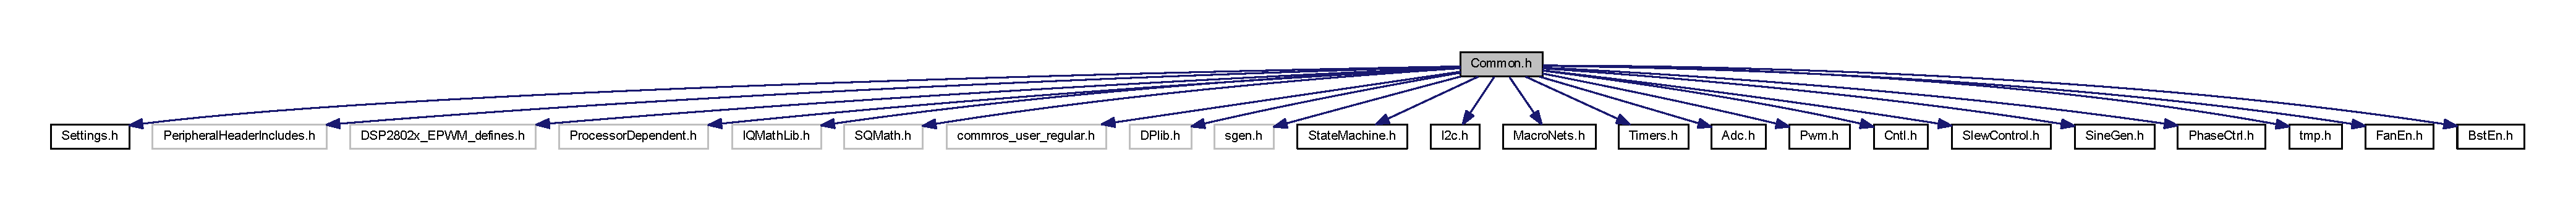
\includegraphics[width=350pt]{_common_8h__incl}
\end{center}
\end{figure}


\subsection{Detailed Description}
Common include file for the project. All other header files used should be included within this file and this file should then be used to include them in the required source files. 
\hypertarget{_fan_en_8h}{\section{Fan\-En.\-h File Reference}
\label{_fan_en_8h}\index{Fan\-En.\-h@{Fan\-En.\-h}}
}


Functions for enabling and disabling the external fans via I2\-C.  


This graph shows which files directly or indirectly include this file\-:\nopagebreak
\begin{figure}[H]
\begin{center}
\leavevmode
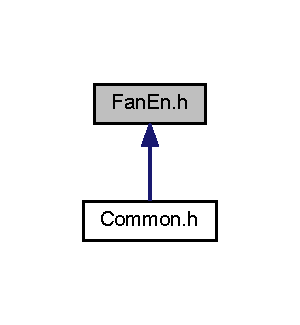
\includegraphics[width=144pt]{_fan_en_8h__dep__incl}
\end{center}
\end{figure}
\subsection*{Macros}
\begin{DoxyCompactItemize}
\item 
\#define \hyperlink{_fan_en_8h_ad615a329bea187ce779cf9930ba8a6fa}{I\-O\-E\-\_\-\-I2\-C\-\_\-\-A\-D\-D\-R}~0x20
\item 
\#define \hyperlink{_fan_en_8h_a36c134b088cc2e64e0a5e14e8f90fe38}{I\-O\-E\-\_\-\-I\-O\-D\-I\-R\-\_\-\-A\-D\-D\-R}~0x00
\item 
\#define \hyperlink{_fan_en_8h_a04633cd2ea7fd0b332e1edf066f674c4}{I\-O\-E\-\_\-\-I\-P\-O\-L\-\_\-\-A\-D\-D\-R}~0x01
\item 
\#define \hyperlink{_fan_en_8h_aa68be5a6ed28fb146600b4fd2d11fafd}{I\-O\-E\-\_\-\-G\-P\-I\-N\-T\-E\-N\-\_\-\-A\-D\-D\-R}~0x02
\item 
\#define \hyperlink{_fan_en_8h_a687e15212e8d4b49c12159dce73eeeab}{I\-O\-E\-\_\-\-D\-E\-F\-V\-A\-L\-\_\-\-A\-D\-D\-R}~0x03
\item 
\#define \hyperlink{_fan_en_8h_a90945d9544eebc892154f1e0443b1407}{I\-O\-E\-\_\-\-I\-N\-T\-C\-O\-N\-\_\-\-A\-D\-D\-R}~0x04
\item 
\#define \hyperlink{_fan_en_8h_af44ed2bf93808aeb932ce9944a942b75}{I\-O\-E\-\_\-\-I\-O\-C\-O\-N\-\_\-\-A\-D\-D\-R}~0x05
\item 
\#define \hyperlink{_fan_en_8h_a91e588d697383f94de2bf7f11d9ecb4b}{I\-O\-E\-\_\-\-G\-P\-P\-U\-\_\-\-A\-D\-D\-R}~0x06
\item 
\#define \hyperlink{_fan_en_8h_a32cac2ad5af58a2562540ec8fc205dd1}{I\-O\-E\-\_\-\-I\-N\-T\-F\-\_\-\-A\-D\-D\-R}~0x07
\item 
\#define \hyperlink{_fan_en_8h_ac0afd8503a8584599cc81f3d9b0a04dc}{I\-O\-E\-\_\-\-I\-N\-T\-C\-A\-P\-\_\-\-A\-D\-D\-R}~0x08
\item 
\#define \hyperlink{_fan_en_8h_af2d85152c5775a221f107d6de547bca1}{I\-O\-E\-\_\-\-G\-P\-I\-O\-\_\-\-A\-D\-D\-R}~0x09
\item 
\#define \hyperlink{_fan_en_8h_ab26864d7372ac11db9c1996842a3cf56}{I\-O\-E\-\_\-\-O\-L\-A\-T\-\_\-\-A\-D\-D\-R}~0x0\-A
\item 
\#define \hyperlink{_fan_en_8h_a24c7360527d594acd521520c99b3de1b}{F\-A\-N\-\_\-\-N\-U\-M\-\_\-\-C\-H\-N\-L}~0x04
\item 
\#define \hyperlink{_fan_en_8h_a8ccf236abd5b2b9bbf73007968077e3d}{F\-A\-N\-\_\-\-C\-H\-N\-L\-\_\-\-O\-F\-S\-T}~0x04
\end{DoxyCompactItemize}
\subsection*{Functions}
\begin{DoxyCompactItemize}
\item 
Uint16 \hyperlink{_fan_en_8h_a3506b5e25346351ce292e2ad256607cc}{fc\-Init} (void)
\item 
Uint16 \hyperlink{_fan_en_8h_a68c8852e37fd686fda74e593ecd71915}{fc\-Enable} (Uint16 chnl)
\item 
Uint16 \hyperlink{_fan_en_8h_ac781d303e240f077d206088806a75ccd}{fc\-Disable} (Uint16 chnl)
\end{DoxyCompactItemize}


\subsection{Detailed Description}
Functions for enabling and disabling the external fans via I2\-C. The fans are controlled via an external I/\-O expander (M\-C\-P23008) that is connected to the I2\-C bus at address 0100x-\/x-\/x where 'x-\/x-\/x' is dependent upon the configuration of resistors R60 -\/ 61 \& R70 -\/ R74.

After \hyperlink{_fan_en_8h_a3506b5e25346351ce292e2ad256607cc}{fc\-Init()} all fans default to disabled.

\begin{DoxyWarning}{Warning}
Before any fan control functions can be used the I2\-C peripheral M\-U\-S\-T be initialised and E\-I\-T\-H\-E\-R \hyperlink{_fan_en_8h_a3506b5e25346351ce292e2ad256607cc}{fc\-Init()} or \hyperlink{_bst_en_8h_aa6cb02a7aacce8671212b21ed6e39863}{bc\-Init()} must be run -\/ \hyperlink{_fan_en_8h_a3506b5e25346351ce292e2ad256607cc}{fc\-Init()} will require the interrupts to be enabled globally.
\end{DoxyWarning}
\begin{DoxySeeAlso}{See Also}
\hyperlink{_i2c_8h_a1e0a81a1ad1fd7710ca189236e3e5476}{i2c\-Init()} 

\hyperlink{_bst_en_8h_aa6cb02a7aacce8671212b21ed6e39863}{bc\-Init()} 
\end{DoxySeeAlso}


\subsection{Macro Definition Documentation}
\hypertarget{_fan_en_8h_a8ccf236abd5b2b9bbf73007968077e3d}{\index{Fan\-En.\-h@{Fan\-En.\-h}!F\-A\-N\-\_\-\-C\-H\-N\-L\-\_\-\-O\-F\-S\-T@{F\-A\-N\-\_\-\-C\-H\-N\-L\-\_\-\-O\-F\-S\-T}}
\index{F\-A\-N\-\_\-\-C\-H\-N\-L\-\_\-\-O\-F\-S\-T@{F\-A\-N\-\_\-\-C\-H\-N\-L\-\_\-\-O\-F\-S\-T}!FanEn.h@{Fan\-En.\-h}}
\subsubsection[{F\-A\-N\-\_\-\-C\-H\-N\-L\-\_\-\-O\-F\-S\-T}]{\setlength{\rightskip}{0pt plus 5cm}\#define F\-A\-N\-\_\-\-C\-H\-N\-L\-\_\-\-O\-F\-S\-T~0x04}}\label{_fan_en_8h_a8ccf236abd5b2b9bbf73007968077e3d}
Fan channel numbering offset \hypertarget{_fan_en_8h_a24c7360527d594acd521520c99b3de1b}{\index{Fan\-En.\-h@{Fan\-En.\-h}!F\-A\-N\-\_\-\-N\-U\-M\-\_\-\-C\-H\-N\-L@{F\-A\-N\-\_\-\-N\-U\-M\-\_\-\-C\-H\-N\-L}}
\index{F\-A\-N\-\_\-\-N\-U\-M\-\_\-\-C\-H\-N\-L@{F\-A\-N\-\_\-\-N\-U\-M\-\_\-\-C\-H\-N\-L}!FanEn.h@{Fan\-En.\-h}}
\subsubsection[{F\-A\-N\-\_\-\-N\-U\-M\-\_\-\-C\-H\-N\-L}]{\setlength{\rightskip}{0pt plus 5cm}\#define F\-A\-N\-\_\-\-N\-U\-M\-\_\-\-C\-H\-N\-L~0x04}}\label{_fan_en_8h_a24c7360527d594acd521520c99b3de1b}
Number of fan channels \hypertarget{_fan_en_8h_a687e15212e8d4b49c12159dce73eeeab}{\index{Fan\-En.\-h@{Fan\-En.\-h}!I\-O\-E\-\_\-\-D\-E\-F\-V\-A\-L\-\_\-\-A\-D\-D\-R@{I\-O\-E\-\_\-\-D\-E\-F\-V\-A\-L\-\_\-\-A\-D\-D\-R}}
\index{I\-O\-E\-\_\-\-D\-E\-F\-V\-A\-L\-\_\-\-A\-D\-D\-R@{I\-O\-E\-\_\-\-D\-E\-F\-V\-A\-L\-\_\-\-A\-D\-D\-R}!FanEn.h@{Fan\-En.\-h}}
\subsubsection[{I\-O\-E\-\_\-\-D\-E\-F\-V\-A\-L\-\_\-\-A\-D\-D\-R}]{\setlength{\rightskip}{0pt plus 5cm}\#define I\-O\-E\-\_\-\-D\-E\-F\-V\-A\-L\-\_\-\-A\-D\-D\-R~0x03}}\label{_fan_en_8h_a687e15212e8d4b49c12159dce73eeeab}
M\-C\-P23008 I/\-O expander default value register address \hypertarget{_fan_en_8h_aa68be5a6ed28fb146600b4fd2d11fafd}{\index{Fan\-En.\-h@{Fan\-En.\-h}!I\-O\-E\-\_\-\-G\-P\-I\-N\-T\-E\-N\-\_\-\-A\-D\-D\-R@{I\-O\-E\-\_\-\-G\-P\-I\-N\-T\-E\-N\-\_\-\-A\-D\-D\-R}}
\index{I\-O\-E\-\_\-\-G\-P\-I\-N\-T\-E\-N\-\_\-\-A\-D\-D\-R@{I\-O\-E\-\_\-\-G\-P\-I\-N\-T\-E\-N\-\_\-\-A\-D\-D\-R}!FanEn.h@{Fan\-En.\-h}}
\subsubsection[{I\-O\-E\-\_\-\-G\-P\-I\-N\-T\-E\-N\-\_\-\-A\-D\-D\-R}]{\setlength{\rightskip}{0pt plus 5cm}\#define I\-O\-E\-\_\-\-G\-P\-I\-N\-T\-E\-N\-\_\-\-A\-D\-D\-R~0x02}}\label{_fan_en_8h_aa68be5a6ed28fb146600b4fd2d11fafd}
M\-C\-P23008 I/\-O expander interrupt on change enable register address \hypertarget{_fan_en_8h_af2d85152c5775a221f107d6de547bca1}{\index{Fan\-En.\-h@{Fan\-En.\-h}!I\-O\-E\-\_\-\-G\-P\-I\-O\-\_\-\-A\-D\-D\-R@{I\-O\-E\-\_\-\-G\-P\-I\-O\-\_\-\-A\-D\-D\-R}}
\index{I\-O\-E\-\_\-\-G\-P\-I\-O\-\_\-\-A\-D\-D\-R@{I\-O\-E\-\_\-\-G\-P\-I\-O\-\_\-\-A\-D\-D\-R}!FanEn.h@{Fan\-En.\-h}}
\subsubsection[{I\-O\-E\-\_\-\-G\-P\-I\-O\-\_\-\-A\-D\-D\-R}]{\setlength{\rightskip}{0pt plus 5cm}\#define I\-O\-E\-\_\-\-G\-P\-I\-O\-\_\-\-A\-D\-D\-R~0x09}}\label{_fan_en_8h_af2d85152c5775a221f107d6de547bca1}
M\-C\-P23008 I/\-O expander G\-P\-I\-O port register address \hypertarget{_fan_en_8h_a91e588d697383f94de2bf7f11d9ecb4b}{\index{Fan\-En.\-h@{Fan\-En.\-h}!I\-O\-E\-\_\-\-G\-P\-P\-U\-\_\-\-A\-D\-D\-R@{I\-O\-E\-\_\-\-G\-P\-P\-U\-\_\-\-A\-D\-D\-R}}
\index{I\-O\-E\-\_\-\-G\-P\-P\-U\-\_\-\-A\-D\-D\-R@{I\-O\-E\-\_\-\-G\-P\-P\-U\-\_\-\-A\-D\-D\-R}!FanEn.h@{Fan\-En.\-h}}
\subsubsection[{I\-O\-E\-\_\-\-G\-P\-P\-U\-\_\-\-A\-D\-D\-R}]{\setlength{\rightskip}{0pt plus 5cm}\#define I\-O\-E\-\_\-\-G\-P\-P\-U\-\_\-\-A\-D\-D\-R~0x06}}\label{_fan_en_8h_a91e588d697383f94de2bf7f11d9ecb4b}
M\-C\-P23008 I/\-O expander pull-\/up resistor configuration register address \hypertarget{_fan_en_8h_ad615a329bea187ce779cf9930ba8a6fa}{\index{Fan\-En.\-h@{Fan\-En.\-h}!I\-O\-E\-\_\-\-I2\-C\-\_\-\-A\-D\-D\-R@{I\-O\-E\-\_\-\-I2\-C\-\_\-\-A\-D\-D\-R}}
\index{I\-O\-E\-\_\-\-I2\-C\-\_\-\-A\-D\-D\-R@{I\-O\-E\-\_\-\-I2\-C\-\_\-\-A\-D\-D\-R}!FanEn.h@{Fan\-En.\-h}}
\subsubsection[{I\-O\-E\-\_\-\-I2\-C\-\_\-\-A\-D\-D\-R}]{\setlength{\rightskip}{0pt plus 5cm}\#define I\-O\-E\-\_\-\-I2\-C\-\_\-\-A\-D\-D\-R~0x20}}\label{_fan_en_8h_ad615a329bea187ce779cf9930ba8a6fa}
M\-C\-P23008 I/\-O expander I2\-C address (slave, 32d, 8-\/bit I/\-O expander) \hypertarget{_fan_en_8h_ac0afd8503a8584599cc81f3d9b0a04dc}{\index{Fan\-En.\-h@{Fan\-En.\-h}!I\-O\-E\-\_\-\-I\-N\-T\-C\-A\-P\-\_\-\-A\-D\-D\-R@{I\-O\-E\-\_\-\-I\-N\-T\-C\-A\-P\-\_\-\-A\-D\-D\-R}}
\index{I\-O\-E\-\_\-\-I\-N\-T\-C\-A\-P\-\_\-\-A\-D\-D\-R@{I\-O\-E\-\_\-\-I\-N\-T\-C\-A\-P\-\_\-\-A\-D\-D\-R}!FanEn.h@{Fan\-En.\-h}}
\subsubsection[{I\-O\-E\-\_\-\-I\-N\-T\-C\-A\-P\-\_\-\-A\-D\-D\-R}]{\setlength{\rightskip}{0pt plus 5cm}\#define I\-O\-E\-\_\-\-I\-N\-T\-C\-A\-P\-\_\-\-A\-D\-D\-R~0x08}}\label{_fan_en_8h_ac0afd8503a8584599cc81f3d9b0a04dc}
M\-C\-P23008 I/\-O expander interrupt capture register address \hypertarget{_fan_en_8h_a90945d9544eebc892154f1e0443b1407}{\index{Fan\-En.\-h@{Fan\-En.\-h}!I\-O\-E\-\_\-\-I\-N\-T\-C\-O\-N\-\_\-\-A\-D\-D\-R@{I\-O\-E\-\_\-\-I\-N\-T\-C\-O\-N\-\_\-\-A\-D\-D\-R}}
\index{I\-O\-E\-\_\-\-I\-N\-T\-C\-O\-N\-\_\-\-A\-D\-D\-R@{I\-O\-E\-\_\-\-I\-N\-T\-C\-O\-N\-\_\-\-A\-D\-D\-R}!FanEn.h@{Fan\-En.\-h}}
\subsubsection[{I\-O\-E\-\_\-\-I\-N\-T\-C\-O\-N\-\_\-\-A\-D\-D\-R}]{\setlength{\rightskip}{0pt plus 5cm}\#define I\-O\-E\-\_\-\-I\-N\-T\-C\-O\-N\-\_\-\-A\-D\-D\-R~0x04}}\label{_fan_en_8h_a90945d9544eebc892154f1e0443b1407}
M\-C\-P23008 I/\-O expander interrupt on change control register address \hypertarget{_fan_en_8h_a32cac2ad5af58a2562540ec8fc205dd1}{\index{Fan\-En.\-h@{Fan\-En.\-h}!I\-O\-E\-\_\-\-I\-N\-T\-F\-\_\-\-A\-D\-D\-R@{I\-O\-E\-\_\-\-I\-N\-T\-F\-\_\-\-A\-D\-D\-R}}
\index{I\-O\-E\-\_\-\-I\-N\-T\-F\-\_\-\-A\-D\-D\-R@{I\-O\-E\-\_\-\-I\-N\-T\-F\-\_\-\-A\-D\-D\-R}!FanEn.h@{Fan\-En.\-h}}
\subsubsection[{I\-O\-E\-\_\-\-I\-N\-T\-F\-\_\-\-A\-D\-D\-R}]{\setlength{\rightskip}{0pt plus 5cm}\#define I\-O\-E\-\_\-\-I\-N\-T\-F\-\_\-\-A\-D\-D\-R~0x07}}\label{_fan_en_8h_a32cac2ad5af58a2562540ec8fc205dd1}
M\-C\-P23008 I/\-O expander interrupt flag register address \hypertarget{_fan_en_8h_af44ed2bf93808aeb932ce9944a942b75}{\index{Fan\-En.\-h@{Fan\-En.\-h}!I\-O\-E\-\_\-\-I\-O\-C\-O\-N\-\_\-\-A\-D\-D\-R@{I\-O\-E\-\_\-\-I\-O\-C\-O\-N\-\_\-\-A\-D\-D\-R}}
\index{I\-O\-E\-\_\-\-I\-O\-C\-O\-N\-\_\-\-A\-D\-D\-R@{I\-O\-E\-\_\-\-I\-O\-C\-O\-N\-\_\-\-A\-D\-D\-R}!FanEn.h@{Fan\-En.\-h}}
\subsubsection[{I\-O\-E\-\_\-\-I\-O\-C\-O\-N\-\_\-\-A\-D\-D\-R}]{\setlength{\rightskip}{0pt plus 5cm}\#define I\-O\-E\-\_\-\-I\-O\-C\-O\-N\-\_\-\-A\-D\-D\-R~0x05}}\label{_fan_en_8h_af44ed2bf93808aeb932ce9944a942b75}
M\-C\-P23008 I/\-O expander configuration register address \hypertarget{_fan_en_8h_a36c134b088cc2e64e0a5e14e8f90fe38}{\index{Fan\-En.\-h@{Fan\-En.\-h}!I\-O\-E\-\_\-\-I\-O\-D\-I\-R\-\_\-\-A\-D\-D\-R@{I\-O\-E\-\_\-\-I\-O\-D\-I\-R\-\_\-\-A\-D\-D\-R}}
\index{I\-O\-E\-\_\-\-I\-O\-D\-I\-R\-\_\-\-A\-D\-D\-R@{I\-O\-E\-\_\-\-I\-O\-D\-I\-R\-\_\-\-A\-D\-D\-R}!FanEn.h@{Fan\-En.\-h}}
\subsubsection[{I\-O\-E\-\_\-\-I\-O\-D\-I\-R\-\_\-\-A\-D\-D\-R}]{\setlength{\rightskip}{0pt plus 5cm}\#define I\-O\-E\-\_\-\-I\-O\-D\-I\-R\-\_\-\-A\-D\-D\-R~0x00}}\label{_fan_en_8h_a36c134b088cc2e64e0a5e14e8f90fe38}
M\-C\-P23008 I/\-O expander I/\-O direction register address \hypertarget{_fan_en_8h_a04633cd2ea7fd0b332e1edf066f674c4}{\index{Fan\-En.\-h@{Fan\-En.\-h}!I\-O\-E\-\_\-\-I\-P\-O\-L\-\_\-\-A\-D\-D\-R@{I\-O\-E\-\_\-\-I\-P\-O\-L\-\_\-\-A\-D\-D\-R}}
\index{I\-O\-E\-\_\-\-I\-P\-O\-L\-\_\-\-A\-D\-D\-R@{I\-O\-E\-\_\-\-I\-P\-O\-L\-\_\-\-A\-D\-D\-R}!FanEn.h@{Fan\-En.\-h}}
\subsubsection[{I\-O\-E\-\_\-\-I\-P\-O\-L\-\_\-\-A\-D\-D\-R}]{\setlength{\rightskip}{0pt plus 5cm}\#define I\-O\-E\-\_\-\-I\-P\-O\-L\-\_\-\-A\-D\-D\-R~0x01}}\label{_fan_en_8h_a04633cd2ea7fd0b332e1edf066f674c4}
M\-C\-P23008 I/\-O expander input polarity register address \hypertarget{_fan_en_8h_ab26864d7372ac11db9c1996842a3cf56}{\index{Fan\-En.\-h@{Fan\-En.\-h}!I\-O\-E\-\_\-\-O\-L\-A\-T\-\_\-\-A\-D\-D\-R@{I\-O\-E\-\_\-\-O\-L\-A\-T\-\_\-\-A\-D\-D\-R}}
\index{I\-O\-E\-\_\-\-O\-L\-A\-T\-\_\-\-A\-D\-D\-R@{I\-O\-E\-\_\-\-O\-L\-A\-T\-\_\-\-A\-D\-D\-R}!FanEn.h@{Fan\-En.\-h}}
\subsubsection[{I\-O\-E\-\_\-\-O\-L\-A\-T\-\_\-\-A\-D\-D\-R}]{\setlength{\rightskip}{0pt plus 5cm}\#define I\-O\-E\-\_\-\-O\-L\-A\-T\-\_\-\-A\-D\-D\-R~0x0\-A}}\label{_fan_en_8h_ab26864d7372ac11db9c1996842a3cf56}
M\-C\-P23008 I/\-O expander output latch register address 

\subsection{Function Documentation}
\hypertarget{_fan_en_8h_ac781d303e240f077d206088806a75ccd}{\index{Fan\-En.\-h@{Fan\-En.\-h}!fc\-Disable@{fc\-Disable}}
\index{fc\-Disable@{fc\-Disable}!FanEn.h@{Fan\-En.\-h}}
\subsubsection[{fc\-Disable}]{\setlength{\rightskip}{0pt plus 5cm}Uint16 fc\-Disable (
\begin{DoxyParamCaption}
\item[{Uint16}]{chnl}
\end{DoxyParamCaption}
)}}\label{_fan_en_8h_ac781d303e240f077d206088806a75ccd}
Disables the specified channel's fan The I2\-C peripheral and the fan enable controller interface M\-U\-S\-T be initialised before this function is used. \begin{DoxySeeAlso}{See Also}
\hyperlink{_i2c_8h_a1e0a81a1ad1fd7710ca189236e3e5476}{i2c\-Init()} 

\hyperlink{_fan_en_8h_a3506b5e25346351ce292e2ad256607cc}{fc\-Init()} 
\end{DoxySeeAlso}

\begin{DoxyParams}[1]{Parameters}
\mbox{\tt in}  & {\em chnl} & Specifies the channel fan that is to be disabled \\
\hline
\end{DoxyParams}
\begin{DoxyReturn}{Returns}
Error status 
\end{DoxyReturn}
\hypertarget{_fan_en_8h_a68c8852e37fd686fda74e593ecd71915}{\index{Fan\-En.\-h@{Fan\-En.\-h}!fc\-Enable@{fc\-Enable}}
\index{fc\-Enable@{fc\-Enable}!FanEn.h@{Fan\-En.\-h}}
\subsubsection[{fc\-Enable}]{\setlength{\rightskip}{0pt plus 5cm}Uint16 fc\-Enable (
\begin{DoxyParamCaption}
\item[{Uint16}]{chnl}
\end{DoxyParamCaption}
)}}\label{_fan_en_8h_a68c8852e37fd686fda74e593ecd71915}
Enables the specified channel's fan The I2\-C peripheral and the fan enable controller interface M\-U\-S\-T be initialised before this function is used. \begin{DoxySeeAlso}{See Also}
\hyperlink{_i2c_8h_a1e0a81a1ad1fd7710ca189236e3e5476}{i2c\-Init()} 

\hyperlink{_fan_en_8h_a3506b5e25346351ce292e2ad256607cc}{fc\-Init()} 
\end{DoxySeeAlso}

\begin{DoxyParams}[1]{Parameters}
\mbox{\tt in}  & {\em chnl} & Specifies the channel fan that is to be enabled \\
\hline
\end{DoxyParams}
\begin{DoxyReturn}{Returns}
Error status 
\end{DoxyReturn}
\hypertarget{_fan_en_8h_a3506b5e25346351ce292e2ad256607cc}{\index{Fan\-En.\-h@{Fan\-En.\-h}!fc\-Init@{fc\-Init}}
\index{fc\-Init@{fc\-Init}!FanEn.h@{Fan\-En.\-h}}
\subsubsection[{fc\-Init}]{\setlength{\rightskip}{0pt plus 5cm}Uint16 fc\-Init (
\begin{DoxyParamCaption}
\item[{void}]{}
\end{DoxyParamCaption}
)}}\label{_fan_en_8h_a3506b5e25346351ce292e2ad256607cc}
Initialises the fan enable control interface. The I2\-C peripheral must be initialised before this function is used. \begin{DoxySeeAlso}{See Also}
\hyperlink{_i2c_8h_a1e0a81a1ad1fd7710ca189236e3e5476}{i2c\-Init()} 
\end{DoxySeeAlso}
\begin{DoxyReturn}{Returns}
Error status 
\end{DoxyReturn}

\hypertarget{_i2c_8h}{\section{I2c.\-h File Reference}
\label{_i2c_8h}\index{I2c.\-h@{I2c.\-h}}
}


I2\-C communication functions.  


This graph shows which files directly or indirectly include this file\-:\nopagebreak
\begin{figure}[H]
\begin{center}
\leavevmode
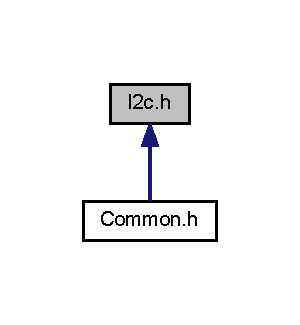
\includegraphics[width=144pt]{_i2c_8h__dep__incl}
\end{center}
\end{figure}
\subsection*{Data Structures}
\begin{DoxyCompactItemize}
\item 
struct \hyperlink{structi2c_msg}{i2c\-Msg}
\end{DoxyCompactItemize}
\subsection*{Macros}
\begin{DoxyCompactItemize}
\item 
\#define \hyperlink{_i2c_8h_a0889ccb6e4a98d6d8a0bf7c009c818e2}{I2\-C\-\_\-\-M\-A\-X\-\_\-\-B\-U\-F\-F\-E\-R\-\_\-\-S\-I\-Z\-E}~0x04
\item 
\#define \hyperlink{_i2c_8h_ae429af928d46f8186343fb3eb550dc92}{I2\-C\-\_\-\-M\-A\-X\-\_\-\-P\-T\-R\-\_\-\-S\-I\-Z\-E}~0x02
\end{DoxyCompactItemize}
{\bf }\par
\begin{DoxyCompactItemize}
\item 
\#define \hyperlink{_i2c_8h_a8e07057d8bd0732259c8b4aba0ccf747}{I2\-C\-\_\-\-C\-L\-R\-\_\-\-A\-L\-\_\-\-B\-I\-T}~0x0001
\item 
\#define \hyperlink{_i2c_8h_ac28843bc51cce0ce461810ff06c1dddc}{I2\-C\-\_\-\-C\-L\-R\-\_\-\-N\-A\-C\-K\-\_\-\-B\-I\-T}~0x0002
\item 
\#define \hyperlink{_i2c_8h_a4496263a3b781866a48a6b7e8fcc1543}{I2\-C\-\_\-\-C\-L\-R\-\_\-\-A\-R\-D\-Y\-\_\-\-B\-I\-T}~0x0004
\item 
\#define \hyperlink{_i2c_8h_a10317717bb3efb7ede2a49999fd161ba}{I2\-C\-\_\-\-C\-L\-R\-\_\-\-R\-R\-D\-Y\-\_\-\-B\-I\-T}~0x0008
\item 
\#define \hyperlink{_i2c_8h_aeb930d2f95f82d333b27b02f9586c3cd}{I2\-C\-\_\-\-C\-L\-R\-\_\-\-S\-C\-D\-\_\-\-B\-I\-T}~0x0020
\end{DoxyCompactItemize}

{\bf }\par
\begin{DoxyCompactItemize}
\item 
\#define \hyperlink{_i2c_8h_adf7bc6e4d458e0b13f0ad26570f04528}{I2\-C\-\_\-\-A\-R\-D\-Y\-\_\-\-I\-S\-R\-C}~0x0003
\item 
\#define \hyperlink{_i2c_8h_aa26238e86d534cda62318e98e1655654}{I2\-C\-\_\-\-S\-C\-D\-\_\-\-I\-S\-R\-C}~0x0006
\end{DoxyCompactItemize}

{\bf }\par
\begin{DoxyCompactItemize}
\item 
\#define \hyperlink{_i2c_8h_ad7ff7f3ddb5fb35b633d558b376cf329}{I2\-C\-\_\-\-M\-S\-G\-S\-T\-A\-T\-\_\-\-I\-N\-A\-C\-T\-I\-V\-E}~0x0000
\item 
\#define \hyperlink{_i2c_8h_a56f7eeab5c8dbbe042a10d1f8ac1ad55}{I2\-C\-\_\-\-M\-S\-G\-S\-T\-A\-T\-\_\-\-S\-E\-N\-D\-\_\-\-W\-I\-T\-H\-S\-T\-O\-P}~0x0010
\item 
\#define \hyperlink{_i2c_8h_a36809495e97c0e8033246b227f9716be}{I2\-C\-\_\-\-M\-S\-G\-S\-T\-A\-T\-\_\-\-W\-R\-I\-T\-E\-\_\-\-B\-U\-S\-Y}~0x0011
\item 
\#define \hyperlink{_i2c_8h_a6b46589e75a5bfdc3c57b0bc30cc8671}{I2\-C\-\_\-\-M\-S\-G\-S\-T\-A\-T\-\_\-\-S\-E\-N\-D\-\_\-\-N\-O\-S\-T\-O\-P}~0x0020
\item 
\#define \hyperlink{_i2c_8h_adbe18b39fde045ed6d51eaa7e17b78e0}{I2\-C\-\_\-\-M\-S\-G\-S\-T\-A\-T\-\_\-\-S\-E\-N\-D\-\_\-\-N\-O\-S\-T\-O\-P\-\_\-\-B\-U\-S\-Y}~0x0021
\item 
\#define \hyperlink{_i2c_8h_adf5a3e5950b5af97d3ec2e40b96c2251}{I2\-C\-\_\-\-M\-S\-G\-S\-T\-A\-T\-\_\-\-R\-E\-S\-T\-A\-R\-T}~0x0022
\item 
\#define \hyperlink{_i2c_8h_a9bd9503fa86f5b4d52aeb21be008064a}{I2\-C\-\_\-\-M\-S\-G\-S\-T\-A\-T\-\_\-\-R\-E\-A\-D\-\_\-\-B\-U\-S\-Y}~0x0023
\end{DoxyCompactItemize}

\subsection*{Functions}
\begin{DoxyCompactItemize}
\item 
void \hyperlink{_i2c_8h_a1e0a81a1ad1fd7710ca189236e3e5476}{i2c\-Init} (void)
\item 
void \hyperlink{_i2c_8h_a9e3198d675e7b65c3652bb5c887a7a64}{i2c\-Pop\-Msg} (\hyperlink{structi2c_msg}{i2c\-Msg} $\ast$msg, Uint16 msg\-Status, Uint16 slave\-Addr, Uint16 num\-Data\-Bytes, Uint16 num\-Slave\-Ptr\-Bytes, Uint16 slave\-Ptr\-Addr\-Hi, Uint16 slave\-Ptr\-Addr\-Lo)
\item 
Uint16 \hyperlink{_i2c_8h_a3813bb8cae6159f7df2672a55be4014b}{i2c\-Write} (\hyperlink{structi2c_msg}{i2c\-Msg} $\ast$msg)
\item 
Uint16 \hyperlink{_i2c_8h_aa681ec1b6413dd7009a6aaf0df2cbac1}{i2c\-Read} (\hyperlink{structi2c_msg}{i2c\-Msg} $\ast$msg)
\end{DoxyCompactItemize}


\subsection{Detailed Description}
I2\-C communication functions. \begin{DoxyWarning}{Warning}
The function \hyperlink{_i2c_8h_a1e0a81a1ad1fd7710ca189236e3e5476}{i2c\-Init()} M\-U\-S\-T be called before any other public I2\-C function is used. This will clear any values already in the I2\-C registers.

Interrupts M\-U\-S\-T be globally enabled for the functions \hyperlink{_i2c_8h_a3813bb8cae6159f7df2672a55be4014b}{i2c\-Write()} and \hyperlink{_i2c_8h_aa681ec1b6413dd7009a6aaf0df2cbac1}{i2c\-Read()} to operate correctly.
\end{DoxyWarning}
\begin{DoxySeeAlso}{See Also}
\hyperlink{_bst_en_8h}{Bst\-En.\-h} 

\hyperlink{_fan_en_8h}{Fan\-En.\-h} 

\hyperlink{_tmp_8h}{Tmp.\-h} 
\end{DoxySeeAlso}


\subsection{Macro Definition Documentation}
\hypertarget{_i2c_8h_adf7bc6e4d458e0b13f0ad26570f04528}{\index{I2c.\-h@{I2c.\-h}!I2\-C\-\_\-\-A\-R\-D\-Y\-\_\-\-I\-S\-R\-C@{I2\-C\-\_\-\-A\-R\-D\-Y\-\_\-\-I\-S\-R\-C}}
\index{I2\-C\-\_\-\-A\-R\-D\-Y\-\_\-\-I\-S\-R\-C@{I2\-C\-\_\-\-A\-R\-D\-Y\-\_\-\-I\-S\-R\-C}!I2c.h@{I2c.\-h}}
\subsubsection[{I2\-C\-\_\-\-A\-R\-D\-Y\-\_\-\-I\-S\-R\-C}]{\setlength{\rightskip}{0pt plus 5cm}\#define I2\-C\-\_\-\-A\-R\-D\-Y\-\_\-\-I\-S\-R\-C~0x0003}}\label{_i2c_8h_adf7bc6e4d458e0b13f0ad26570f04528}
I2\-C Interrupt Sources Register access ready condition I2\-C interrupt source. \hypertarget{_i2c_8h_a8e07057d8bd0732259c8b4aba0ccf747}{\index{I2c.\-h@{I2c.\-h}!I2\-C\-\_\-\-C\-L\-R\-\_\-\-A\-L\-\_\-\-B\-I\-T@{I2\-C\-\_\-\-C\-L\-R\-\_\-\-A\-L\-\_\-\-B\-I\-T}}
\index{I2\-C\-\_\-\-C\-L\-R\-\_\-\-A\-L\-\_\-\-B\-I\-T@{I2\-C\-\_\-\-C\-L\-R\-\_\-\-A\-L\-\_\-\-B\-I\-T}!I2c.h@{I2c.\-h}}
\subsubsection[{I2\-C\-\_\-\-C\-L\-R\-\_\-\-A\-L\-\_\-\-B\-I\-T}]{\setlength{\rightskip}{0pt plus 5cm}\#define I2\-C\-\_\-\-C\-L\-R\-\_\-\-A\-L\-\_\-\-B\-I\-T~0x0001}}\label{_i2c_8h_a8e07057d8bd0732259c8b4aba0ccf747}
I2\-C Status Clear Bits Arbitration lost status clear bit. \hypertarget{_i2c_8h_a4496263a3b781866a48a6b7e8fcc1543}{\index{I2c.\-h@{I2c.\-h}!I2\-C\-\_\-\-C\-L\-R\-\_\-\-A\-R\-D\-Y\-\_\-\-B\-I\-T@{I2\-C\-\_\-\-C\-L\-R\-\_\-\-A\-R\-D\-Y\-\_\-\-B\-I\-T}}
\index{I2\-C\-\_\-\-C\-L\-R\-\_\-\-A\-R\-D\-Y\-\_\-\-B\-I\-T@{I2\-C\-\_\-\-C\-L\-R\-\_\-\-A\-R\-D\-Y\-\_\-\-B\-I\-T}!I2c.h@{I2c.\-h}}
\subsubsection[{I2\-C\-\_\-\-C\-L\-R\-\_\-\-A\-R\-D\-Y\-\_\-\-B\-I\-T}]{\setlength{\rightskip}{0pt plus 5cm}\#define I2\-C\-\_\-\-C\-L\-R\-\_\-\-A\-R\-D\-Y\-\_\-\-B\-I\-T~0x0004}}\label{_i2c_8h_a4496263a3b781866a48a6b7e8fcc1543}
Register access ready status clear bit. \hypertarget{_i2c_8h_ac28843bc51cce0ce461810ff06c1dddc}{\index{I2c.\-h@{I2c.\-h}!I2\-C\-\_\-\-C\-L\-R\-\_\-\-N\-A\-C\-K\-\_\-\-B\-I\-T@{I2\-C\-\_\-\-C\-L\-R\-\_\-\-N\-A\-C\-K\-\_\-\-B\-I\-T}}
\index{I2\-C\-\_\-\-C\-L\-R\-\_\-\-N\-A\-C\-K\-\_\-\-B\-I\-T@{I2\-C\-\_\-\-C\-L\-R\-\_\-\-N\-A\-C\-K\-\_\-\-B\-I\-T}!I2c.h@{I2c.\-h}}
\subsubsection[{I2\-C\-\_\-\-C\-L\-R\-\_\-\-N\-A\-C\-K\-\_\-\-B\-I\-T}]{\setlength{\rightskip}{0pt plus 5cm}\#define I2\-C\-\_\-\-C\-L\-R\-\_\-\-N\-A\-C\-K\-\_\-\-B\-I\-T~0x0002}}\label{_i2c_8h_ac28843bc51cce0ce461810ff06c1dddc}
N\-A\-C\-K status clear bit. \hypertarget{_i2c_8h_a10317717bb3efb7ede2a49999fd161ba}{\index{I2c.\-h@{I2c.\-h}!I2\-C\-\_\-\-C\-L\-R\-\_\-\-R\-R\-D\-Y\-\_\-\-B\-I\-T@{I2\-C\-\_\-\-C\-L\-R\-\_\-\-R\-R\-D\-Y\-\_\-\-B\-I\-T}}
\index{I2\-C\-\_\-\-C\-L\-R\-\_\-\-R\-R\-D\-Y\-\_\-\-B\-I\-T@{I2\-C\-\_\-\-C\-L\-R\-\_\-\-R\-R\-D\-Y\-\_\-\-B\-I\-T}!I2c.h@{I2c.\-h}}
\subsubsection[{I2\-C\-\_\-\-C\-L\-R\-\_\-\-R\-R\-D\-Y\-\_\-\-B\-I\-T}]{\setlength{\rightskip}{0pt plus 5cm}\#define I2\-C\-\_\-\-C\-L\-R\-\_\-\-R\-R\-D\-Y\-\_\-\-B\-I\-T~0x0008}}\label{_i2c_8h_a10317717bb3efb7ede2a49999fd161ba}
Receive data ready status clear bit. \hypertarget{_i2c_8h_aeb930d2f95f82d333b27b02f9586c3cd}{\index{I2c.\-h@{I2c.\-h}!I2\-C\-\_\-\-C\-L\-R\-\_\-\-S\-C\-D\-\_\-\-B\-I\-T@{I2\-C\-\_\-\-C\-L\-R\-\_\-\-S\-C\-D\-\_\-\-B\-I\-T}}
\index{I2\-C\-\_\-\-C\-L\-R\-\_\-\-S\-C\-D\-\_\-\-B\-I\-T@{I2\-C\-\_\-\-C\-L\-R\-\_\-\-S\-C\-D\-\_\-\-B\-I\-T}!I2c.h@{I2c.\-h}}
\subsubsection[{I2\-C\-\_\-\-C\-L\-R\-\_\-\-S\-C\-D\-\_\-\-B\-I\-T}]{\setlength{\rightskip}{0pt plus 5cm}\#define I2\-C\-\_\-\-C\-L\-R\-\_\-\-S\-C\-D\-\_\-\-B\-I\-T~0x0020}}\label{_i2c_8h_aeb930d2f95f82d333b27b02f9586c3cd}
Stop detected status clear bit. \hypertarget{_i2c_8h_a0889ccb6e4a98d6d8a0bf7c009c818e2}{\index{I2c.\-h@{I2c.\-h}!I2\-C\-\_\-\-M\-A\-X\-\_\-\-B\-U\-F\-F\-E\-R\-\_\-\-S\-I\-Z\-E@{I2\-C\-\_\-\-M\-A\-X\-\_\-\-B\-U\-F\-F\-E\-R\-\_\-\-S\-I\-Z\-E}}
\index{I2\-C\-\_\-\-M\-A\-X\-\_\-\-B\-U\-F\-F\-E\-R\-\_\-\-S\-I\-Z\-E@{I2\-C\-\_\-\-M\-A\-X\-\_\-\-B\-U\-F\-F\-E\-R\-\_\-\-S\-I\-Z\-E}!I2c.h@{I2c.\-h}}
\subsubsection[{I2\-C\-\_\-\-M\-A\-X\-\_\-\-B\-U\-F\-F\-E\-R\-\_\-\-S\-I\-Z\-E}]{\setlength{\rightskip}{0pt plus 5cm}\#define I2\-C\-\_\-\-M\-A\-X\-\_\-\-B\-U\-F\-F\-E\-R\-\_\-\-S\-I\-Z\-E~0x04}}\label{_i2c_8h_a0889ccb6e4a98d6d8a0bf7c009c818e2}
Maximum I2\-C message buffer size in bytes, including slave register pointer bytes. \hypertarget{_i2c_8h_ae429af928d46f8186343fb3eb550dc92}{\index{I2c.\-h@{I2c.\-h}!I2\-C\-\_\-\-M\-A\-X\-\_\-\-P\-T\-R\-\_\-\-S\-I\-Z\-E@{I2\-C\-\_\-\-M\-A\-X\-\_\-\-P\-T\-R\-\_\-\-S\-I\-Z\-E}}
\index{I2\-C\-\_\-\-M\-A\-X\-\_\-\-P\-T\-R\-\_\-\-S\-I\-Z\-E@{I2\-C\-\_\-\-M\-A\-X\-\_\-\-P\-T\-R\-\_\-\-S\-I\-Z\-E}!I2c.h@{I2c.\-h}}
\subsubsection[{I2\-C\-\_\-\-M\-A\-X\-\_\-\-P\-T\-R\-\_\-\-S\-I\-Z\-E}]{\setlength{\rightskip}{0pt plus 5cm}\#define I2\-C\-\_\-\-M\-A\-X\-\_\-\-P\-T\-R\-\_\-\-S\-I\-Z\-E~0x02}}\label{_i2c_8h_ae429af928d46f8186343fb3eb550dc92}
Maximum number of slave register pointer bytes. \hypertarget{_i2c_8h_ad7ff7f3ddb5fb35b633d558b376cf329}{\index{I2c.\-h@{I2c.\-h}!I2\-C\-\_\-\-M\-S\-G\-S\-T\-A\-T\-\_\-\-I\-N\-A\-C\-T\-I\-V\-E@{I2\-C\-\_\-\-M\-S\-G\-S\-T\-A\-T\-\_\-\-I\-N\-A\-C\-T\-I\-V\-E}}
\index{I2\-C\-\_\-\-M\-S\-G\-S\-T\-A\-T\-\_\-\-I\-N\-A\-C\-T\-I\-V\-E@{I2\-C\-\_\-\-M\-S\-G\-S\-T\-A\-T\-\_\-\-I\-N\-A\-C\-T\-I\-V\-E}!I2c.h@{I2c.\-h}}
\subsubsection[{I2\-C\-\_\-\-M\-S\-G\-S\-T\-A\-T\-\_\-\-I\-N\-A\-C\-T\-I\-V\-E}]{\setlength{\rightskip}{0pt plus 5cm}\#define I2\-C\-\_\-\-M\-S\-G\-S\-T\-A\-T\-\_\-\-I\-N\-A\-C\-T\-I\-V\-E~0x0000}}\label{_i2c_8h_ad7ff7f3ddb5fb35b633d558b376cf329}
I2\-C Message States Inactive I2\-C message state. \hypertarget{_i2c_8h_a9bd9503fa86f5b4d52aeb21be008064a}{\index{I2c.\-h@{I2c.\-h}!I2\-C\-\_\-\-M\-S\-G\-S\-T\-A\-T\-\_\-\-R\-E\-A\-D\-\_\-\-B\-U\-S\-Y@{I2\-C\-\_\-\-M\-S\-G\-S\-T\-A\-T\-\_\-\-R\-E\-A\-D\-\_\-\-B\-U\-S\-Y}}
\index{I2\-C\-\_\-\-M\-S\-G\-S\-T\-A\-T\-\_\-\-R\-E\-A\-D\-\_\-\-B\-U\-S\-Y@{I2\-C\-\_\-\-M\-S\-G\-S\-T\-A\-T\-\_\-\-R\-E\-A\-D\-\_\-\-B\-U\-S\-Y}!I2c.h@{I2c.\-h}}
\subsubsection[{I2\-C\-\_\-\-M\-S\-G\-S\-T\-A\-T\-\_\-\-R\-E\-A\-D\-\_\-\-B\-U\-S\-Y}]{\setlength{\rightskip}{0pt plus 5cm}\#define I2\-C\-\_\-\-M\-S\-G\-S\-T\-A\-T\-\_\-\-R\-E\-A\-D\-\_\-\-B\-U\-S\-Y~0x0023}}\label{_i2c_8h_a9bd9503fa86f5b4d52aeb21be008064a}
State indicating the I2\-C is busy with a read. \hypertarget{_i2c_8h_adf5a3e5950b5af97d3ec2e40b96c2251}{\index{I2c.\-h@{I2c.\-h}!I2\-C\-\_\-\-M\-S\-G\-S\-T\-A\-T\-\_\-\-R\-E\-S\-T\-A\-R\-T@{I2\-C\-\_\-\-M\-S\-G\-S\-T\-A\-T\-\_\-\-R\-E\-S\-T\-A\-R\-T}}
\index{I2\-C\-\_\-\-M\-S\-G\-S\-T\-A\-T\-\_\-\-R\-E\-S\-T\-A\-R\-T@{I2\-C\-\_\-\-M\-S\-G\-S\-T\-A\-T\-\_\-\-R\-E\-S\-T\-A\-R\-T}!I2c.h@{I2c.\-h}}
\subsubsection[{I2\-C\-\_\-\-M\-S\-G\-S\-T\-A\-T\-\_\-\-R\-E\-S\-T\-A\-R\-T}]{\setlength{\rightskip}{0pt plus 5cm}\#define I2\-C\-\_\-\-M\-S\-G\-S\-T\-A\-T\-\_\-\-R\-E\-S\-T\-A\-R\-T~0x0022}}\label{_i2c_8h_adf5a3e5950b5af97d3ec2e40b96c2251}
Transmit a master read with a restart. \hypertarget{_i2c_8h_a6b46589e75a5bfdc3c57b0bc30cc8671}{\index{I2c.\-h@{I2c.\-h}!I2\-C\-\_\-\-M\-S\-G\-S\-T\-A\-T\-\_\-\-S\-E\-N\-D\-\_\-\-N\-O\-S\-T\-O\-P@{I2\-C\-\_\-\-M\-S\-G\-S\-T\-A\-T\-\_\-\-S\-E\-N\-D\-\_\-\-N\-O\-S\-T\-O\-P}}
\index{I2\-C\-\_\-\-M\-S\-G\-S\-T\-A\-T\-\_\-\-S\-E\-N\-D\-\_\-\-N\-O\-S\-T\-O\-P@{I2\-C\-\_\-\-M\-S\-G\-S\-T\-A\-T\-\_\-\-S\-E\-N\-D\-\_\-\-N\-O\-S\-T\-O\-P}!I2c.h@{I2c.\-h}}
\subsubsection[{I2\-C\-\_\-\-M\-S\-G\-S\-T\-A\-T\-\_\-\-S\-E\-N\-D\-\_\-\-N\-O\-S\-T\-O\-P}]{\setlength{\rightskip}{0pt plus 5cm}\#define I2\-C\-\_\-\-M\-S\-G\-S\-T\-A\-T\-\_\-\-S\-E\-N\-D\-\_\-\-N\-O\-S\-T\-O\-P~0x0020}}\label{_i2c_8h_a6b46589e75a5bfdc3c57b0bc30cc8671}
Transmit a write with no stop. \hypertarget{_i2c_8h_adbe18b39fde045ed6d51eaa7e17b78e0}{\index{I2c.\-h@{I2c.\-h}!I2\-C\-\_\-\-M\-S\-G\-S\-T\-A\-T\-\_\-\-S\-E\-N\-D\-\_\-\-N\-O\-S\-T\-O\-P\-\_\-\-B\-U\-S\-Y@{I2\-C\-\_\-\-M\-S\-G\-S\-T\-A\-T\-\_\-\-S\-E\-N\-D\-\_\-\-N\-O\-S\-T\-O\-P\-\_\-\-B\-U\-S\-Y}}
\index{I2\-C\-\_\-\-M\-S\-G\-S\-T\-A\-T\-\_\-\-S\-E\-N\-D\-\_\-\-N\-O\-S\-T\-O\-P\-\_\-\-B\-U\-S\-Y@{I2\-C\-\_\-\-M\-S\-G\-S\-T\-A\-T\-\_\-\-S\-E\-N\-D\-\_\-\-N\-O\-S\-T\-O\-P\-\_\-\-B\-U\-S\-Y}!I2c.h@{I2c.\-h}}
\subsubsection[{I2\-C\-\_\-\-M\-S\-G\-S\-T\-A\-T\-\_\-\-S\-E\-N\-D\-\_\-\-N\-O\-S\-T\-O\-P\-\_\-\-B\-U\-S\-Y}]{\setlength{\rightskip}{0pt plus 5cm}\#define I2\-C\-\_\-\-M\-S\-G\-S\-T\-A\-T\-\_\-\-S\-E\-N\-D\-\_\-\-N\-O\-S\-T\-O\-P\-\_\-\-B\-U\-S\-Y~0x0021}}\label{_i2c_8h_adbe18b39fde045ed6d51eaa7e17b78e0}
State indicating the I2\-C is busy with a write with no stop. \hypertarget{_i2c_8h_a56f7eeab5c8dbbe042a10d1f8ac1ad55}{\index{I2c.\-h@{I2c.\-h}!I2\-C\-\_\-\-M\-S\-G\-S\-T\-A\-T\-\_\-\-S\-E\-N\-D\-\_\-\-W\-I\-T\-H\-S\-T\-O\-P@{I2\-C\-\_\-\-M\-S\-G\-S\-T\-A\-T\-\_\-\-S\-E\-N\-D\-\_\-\-W\-I\-T\-H\-S\-T\-O\-P}}
\index{I2\-C\-\_\-\-M\-S\-G\-S\-T\-A\-T\-\_\-\-S\-E\-N\-D\-\_\-\-W\-I\-T\-H\-S\-T\-O\-P@{I2\-C\-\_\-\-M\-S\-G\-S\-T\-A\-T\-\_\-\-S\-E\-N\-D\-\_\-\-W\-I\-T\-H\-S\-T\-O\-P}!I2c.h@{I2c.\-h}}
\subsubsection[{I2\-C\-\_\-\-M\-S\-G\-S\-T\-A\-T\-\_\-\-S\-E\-N\-D\-\_\-\-W\-I\-T\-H\-S\-T\-O\-P}]{\setlength{\rightskip}{0pt plus 5cm}\#define I2\-C\-\_\-\-M\-S\-G\-S\-T\-A\-T\-\_\-\-S\-E\-N\-D\-\_\-\-W\-I\-T\-H\-S\-T\-O\-P~0x0010}}\label{_i2c_8h_a56f7eeab5c8dbbe042a10d1f8ac1ad55}
Transmit a write with stop I2\-C message state. \hypertarget{_i2c_8h_a36809495e97c0e8033246b227f9716be}{\index{I2c.\-h@{I2c.\-h}!I2\-C\-\_\-\-M\-S\-G\-S\-T\-A\-T\-\_\-\-W\-R\-I\-T\-E\-\_\-\-B\-U\-S\-Y@{I2\-C\-\_\-\-M\-S\-G\-S\-T\-A\-T\-\_\-\-W\-R\-I\-T\-E\-\_\-\-B\-U\-S\-Y}}
\index{I2\-C\-\_\-\-M\-S\-G\-S\-T\-A\-T\-\_\-\-W\-R\-I\-T\-E\-\_\-\-B\-U\-S\-Y@{I2\-C\-\_\-\-M\-S\-G\-S\-T\-A\-T\-\_\-\-W\-R\-I\-T\-E\-\_\-\-B\-U\-S\-Y}!I2c.h@{I2c.\-h}}
\subsubsection[{I2\-C\-\_\-\-M\-S\-G\-S\-T\-A\-T\-\_\-\-W\-R\-I\-T\-E\-\_\-\-B\-U\-S\-Y}]{\setlength{\rightskip}{0pt plus 5cm}\#define I2\-C\-\_\-\-M\-S\-G\-S\-T\-A\-T\-\_\-\-W\-R\-I\-T\-E\-\_\-\-B\-U\-S\-Y~0x0011}}\label{_i2c_8h_a36809495e97c0e8033246b227f9716be}
State indicating the I2\-C is busy with a write with a stop. \hypertarget{_i2c_8h_aa26238e86d534cda62318e98e1655654}{\index{I2c.\-h@{I2c.\-h}!I2\-C\-\_\-\-S\-C\-D\-\_\-\-I\-S\-R\-C@{I2\-C\-\_\-\-S\-C\-D\-\_\-\-I\-S\-R\-C}}
\index{I2\-C\-\_\-\-S\-C\-D\-\_\-\-I\-S\-R\-C@{I2\-C\-\_\-\-S\-C\-D\-\_\-\-I\-S\-R\-C}!I2c.h@{I2c.\-h}}
\subsubsection[{I2\-C\-\_\-\-S\-C\-D\-\_\-\-I\-S\-R\-C}]{\setlength{\rightskip}{0pt plus 5cm}\#define I2\-C\-\_\-\-S\-C\-D\-\_\-\-I\-S\-R\-C~0x0006}}\label{_i2c_8h_aa26238e86d534cda62318e98e1655654}
Stop detected condition I2\-C interrupt source. 

\subsection{Function Documentation}
\hypertarget{_i2c_8h_a1e0a81a1ad1fd7710ca189236e3e5476}{\index{I2c.\-h@{I2c.\-h}!i2c\-Init@{i2c\-Init}}
\index{i2c\-Init@{i2c\-Init}!I2c.h@{I2c.\-h}}
\subsubsection[{i2c\-Init}]{\setlength{\rightskip}{0pt plus 5cm}void i2c\-Init (
\begin{DoxyParamCaption}
\item[{void}]{}
\end{DoxyParamCaption}
)}}\label{_i2c_8h_a1e0a81a1ad1fd7710ca189236e3e5476}
Initialises the I2\-C-\/\-A peripheral and relevant interrupts. This function will clear any values already in the I2\-C peripheral registers. This function M\-U\-S\-T be called before any other public I2\-C function. \hypertarget{_i2c_8h_a9e3198d675e7b65c3652bb5c887a7a64}{\index{I2c.\-h@{I2c.\-h}!i2c\-Pop\-Msg@{i2c\-Pop\-Msg}}
\index{i2c\-Pop\-Msg@{i2c\-Pop\-Msg}!I2c.h@{I2c.\-h}}
\subsubsection[{i2c\-Pop\-Msg}]{\setlength{\rightskip}{0pt plus 5cm}void i2c\-Pop\-Msg (
\begin{DoxyParamCaption}
\item[{{\bf i2c\-Msg} $\ast$}]{msg, }
\item[{Uint16}]{msg\-Status, }
\item[{Uint16}]{slave\-Addr, }
\item[{Uint16}]{num\-Data\-Bytes, }
\item[{Uint16}]{num\-Slave\-Ptr\-Bytes, }
\item[{Uint16}]{slave\-Ptr\-Addr\-Hi, }
\item[{Uint16}]{slave\-Ptr\-Addr\-Lo}
\end{DoxyParamCaption}
)}}\label{_i2c_8h_a9e3198d675e7b65c3652bb5c887a7a64}
This function can be used to validate and populate the specified settings and values into the specified I2\-C message structure. 
\begin{DoxyParams}[1]{Parameters}
\mbox{\tt out}  & {\em msg} & The I2\-C message structure. \\
\hline
\mbox{\tt in}  & {\em msg\-Status} & The initial I2\-C message status. \\
\hline
\mbox{\tt in}  & {\em slave\-Addr} & The slave address. \\
\hline
\mbox{\tt in}  & {\em num\-Data\-Bytes} & The number, if any, of data bytes, above any slave register pointer bytes, in the message. \\
\hline
\mbox{\tt in}  & {\em num\-Slave\-Ptr\-Bytes} & The number, if any, of slave register pointer bytes. \\
\hline
\mbox{\tt in}  & {\em slave\-Ptr\-Addr\-Hi} & The slave register pointer high byte. If only one byte, or none, (as indicated by num\-Slave\-Ptrbytes) is to be used leave this at zero. \\
\hline
\mbox{\tt in}  & {\em slave\-Ptr\-Addr\-Lo} & The slave register pointer low byte. If no pointer bytes (as indicated by num\-Slave\-Ptrbytes) are used leave this at zero. \\
\hline
\end{DoxyParams}
\hypertarget{_i2c_8h_aa681ec1b6413dd7009a6aaf0df2cbac1}{\index{I2c.\-h@{I2c.\-h}!i2c\-Read@{i2c\-Read}}
\index{i2c\-Read@{i2c\-Read}!I2c.h@{I2c.\-h}}
\subsubsection[{i2c\-Read}]{\setlength{\rightskip}{0pt plus 5cm}Uint16 i2c\-Read (
\begin{DoxyParamCaption}
\item[{{\bf i2c\-Msg} $\ast$}]{msg}
\end{DoxyParamCaption}
)}}\label{_i2c_8h_aa681ec1b6413dd7009a6aaf0df2cbac1}
Starts an I2\-C-\/\-Aread using the settings specified. Read bytes are saved to the buffer msg.\-msg\-Buffer\mbox{[}\mbox{]}. 
\begin{DoxyParams}[1]{Parameters}
\mbox{\tt in}  & {\em msg} & The I2\-C message struct. \\
\hline
\end{DoxyParams}
\begin{DoxyReturn}{Returns}
Error status. 
\end{DoxyReturn}
\hypertarget{_i2c_8h_a3813bb8cae6159f7df2672a55be4014b}{\index{I2c.\-h@{I2c.\-h}!i2c\-Write@{i2c\-Write}}
\index{i2c\-Write@{i2c\-Write}!I2c.h@{I2c.\-h}}
\subsubsection[{i2c\-Write}]{\setlength{\rightskip}{0pt plus 5cm}Uint16 i2c\-Write (
\begin{DoxyParamCaption}
\item[{{\bf i2c\-Msg} $\ast$}]{msg}
\end{DoxyParamCaption}
)}}\label{_i2c_8h_a3813bb8cae6159f7df2672a55be4014b}
Starts an I2\-C-\/\-A write using the settings and values specified. 
\begin{DoxyParams}[1]{Parameters}
\mbox{\tt in}  & {\em msg} & The I2\-C message structure. \\
\hline
\end{DoxyParams}
\begin{DoxyReturn}{Returns}
Error Status. 
\end{DoxyReturn}

\hypertarget{_macro_nets_8h}{\section{Macro\-Nets.\-h File Reference}
\label{_macro_nets_8h}\index{Macro\-Nets.\-h@{Macro\-Nets.\-h}}
}


D\-P\-Lib macro net and value control functions.  


This graph shows which files directly or indirectly include this file\-:
\nopagebreak
\begin{figure}[H]
\begin{center}
\leavevmode
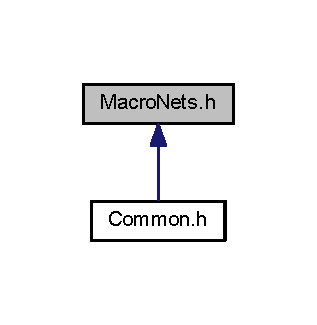
\includegraphics[width=152pt]{_macro_nets_8h__dep__incl}
\end{center}
\end{figure}
\subsection*{Data Structures}
\begin{DoxyCompactItemize}
\item 
struct \hyperlink{structchannel_parameters}{channel\-Parameters}
\end{DoxyCompactItemize}
\subsection*{Macros}
\begin{DoxyCompactItemize}
\item 
\#define \hyperlink{_macro_nets_8h_a007a209cd2e2b935be1f69218652edc1}{L\-O\-A\-D\-\_\-0}~0
\item 
\#define \hyperlink{_macro_nets_8h_a363f09c63f2ecb9086b47d72a3f3f57d}{L\-O\-A\-D\-\_\-1}~1
\item 
\#define \hyperlink{_macro_nets_8h_af7c1e96216e7b48160e5a03afe8ac807}{L\-O\-A\-D\-\_\-2}~2
\item 
\#define \hyperlink{_macro_nets_8h_a2c862ec4115c4a016b61800609f236a7}{L\-O\-A\-D\-\_\-3}~3
\item 
\#define \hyperlink{_macro_nets_8h_ab875424e7a295e6a0eae1605b3285adb}{A\-C\-\_\-\-I\-\_\-\-C\-N\-T\-L}~4
\item 
\#define \hyperlink{_macro_nets_8h_af3967a451ed4068ca1cbf55dd2de3799}{D\-C\-\_\-\-S\-T\-A\-G\-E}~5
\item 
\#define \hyperlink{_macro_nets_8h_a3fc4318ae73eae35339f616047300b0f}{A\-C\-\_\-\-S\-T\-A\-G\-E}~6
\item 
\#define \hyperlink{_macro_nets_8h_a1ae2d3caef45c64fbb9175c50c27ce09}{V\-\_\-\-M\-I\-D\-\_\-\-C\-H}~7
\end{DoxyCompactItemize}
\subsection*{Typedefs}
\begin{DoxyCompactItemize}
\item 
typedef enum \hyperlink{_macro_nets_8h_a067edf486f2115dfa74e51ce43cfdfa6}{ac\-Or\-Dc} \hyperlink{_macro_nets_8h_acd90d47e6937efc4183ab0d18f787575}{op\-Type}
\item 
typedef enum \hyperlink{_macro_nets_8h_a717a050513c9f1668fa40e08c4d5e78f}{i\-Or\-V\-Ctl} \hyperlink{_macro_nets_8h_a5cd368998e9721e657fd7bc6d413807a}{ctl\-Type}
\end{DoxyCompactItemize}
\subsection*{Enumerations}
\begin{DoxyCompactItemize}
\item 
enum \hyperlink{_macro_nets_8h_a067edf486f2115dfa74e51ce43cfdfa6}{ac\-Or\-Dc} \{ \hyperlink{_macro_nets_8h_a067edf486f2115dfa74e51ce43cfdfa6a22e2e72997ac4289587cadae38cc561e}{dc} = 0, 
\hyperlink{_macro_nets_8h_a067edf486f2115dfa74e51ce43cfdfa6ae13614f9b874b4bbeb45317b280ae5f0}{ac} = 1
 \}
\item 
enum \hyperlink{_macro_nets_8h_a717a050513c9f1668fa40e08c4d5e78f}{i\-Or\-V\-Ctl} \{ \hyperlink{_macro_nets_8h_a717a050513c9f1668fa40e08c4d5e78fad6554a2c0fc85e1b2dd381d6802c9052}{i\-Ctrl} = 0, 
\hyperlink{_macro_nets_8h_a717a050513c9f1668fa40e08c4d5e78fa0ea2edd69d870d99d3d8c102cd058383}{v\-Ctrl} = 1
 \}
\end{DoxyCompactItemize}
\subsection*{Functions}
\begin{DoxyCompactItemize}
\item 
void \hyperlink{_macro_nets_8h_ab787ed8809b8f3c22f698937c4f06fd7}{mn\-Setup\-Channels} (void)
\item 
void \hyperlink{_macro_nets_8h_a06d36d85b8d9d27cfc6674244ef1e603}{mn\-Connect\-Nets} (void)
\item 
void \hyperlink{_macro_nets_8h_ab9e9d895e2dd716625fbd464e944071c}{mn\-Stop\-All} (void)
\item 
void \hyperlink{_macro_nets_8h_a1e41564c4405fd553d1fed9cb2dbdda5}{mn\-Run\-All} (void)
\end{DoxyCompactItemize}
\subsection*{Variables}
\begin{DoxyCompactItemize}
\item 
Uint16 \hyperlink{_macro_nets_8h_ac9eb1cb01cb0229168d4277ac4c08295}{stop\-All}
\item 
Uint16 \hyperlink{_macro_nets_8h_a002da2ac651ab8bfc5755c0cd454a64f}{enable\-All}
\item 
\hyperlink{structchannel_parameters}{channel\-Parameters} \hyperlink{_macro_nets_8h_a8d5dc394c7de43ab47a4f709a03331b9}{channel} \mbox{[}\hyperlink{_settings_8h_afe433b138bb71d8d26b6e0907e656d1b}{N\-U\-M\-\_\-\-C\-H\-N\-L\-S}+1\mbox{]}
\end{DoxyCompactItemize}


\subsection{Detailed Description}
D\-P\-Lib macro net and value control functions. 

\subsection{Macro Definition Documentation}
\hypertarget{_macro_nets_8h_ab875424e7a295e6a0eae1605b3285adb}{\index{Macro\-Nets.\-h@{Macro\-Nets.\-h}!A\-C\-\_\-\-I\-\_\-\-C\-N\-T\-L@{A\-C\-\_\-\-I\-\_\-\-C\-N\-T\-L}}
\index{A\-C\-\_\-\-I\-\_\-\-C\-N\-T\-L@{A\-C\-\_\-\-I\-\_\-\-C\-N\-T\-L}!MacroNets.h@{Macro\-Nets.\-h}}
\subsubsection[{A\-C\-\_\-\-I\-\_\-\-C\-N\-T\-L}]{\setlength{\rightskip}{0pt plus 5cm}\#define A\-C\-\_\-\-I\-\_\-\-C\-N\-T\-L~4}}\label{_macro_nets_8h_ab875424e7a295e6a0eae1605b3285adb}
The index position for A\-C I control settings. \hypertarget{_macro_nets_8h_a3fc4318ae73eae35339f616047300b0f}{\index{Macro\-Nets.\-h@{Macro\-Nets.\-h}!A\-C\-\_\-\-S\-T\-A\-G\-E@{A\-C\-\_\-\-S\-T\-A\-G\-E}}
\index{A\-C\-\_\-\-S\-T\-A\-G\-E@{A\-C\-\_\-\-S\-T\-A\-G\-E}!MacroNets.h@{Macro\-Nets.\-h}}
\subsubsection[{A\-C\-\_\-\-S\-T\-A\-G\-E}]{\setlength{\rightskip}{0pt plus 5cm}\#define A\-C\-\_\-\-S\-T\-A\-G\-E~6}}\label{_macro_nets_8h_a3fc4318ae73eae35339f616047300b0f}
The index position for A\-C stage settings. \hypertarget{_macro_nets_8h_af3967a451ed4068ca1cbf55dd2de3799}{\index{Macro\-Nets.\-h@{Macro\-Nets.\-h}!D\-C\-\_\-\-S\-T\-A\-G\-E@{D\-C\-\_\-\-S\-T\-A\-G\-E}}
\index{D\-C\-\_\-\-S\-T\-A\-G\-E@{D\-C\-\_\-\-S\-T\-A\-G\-E}!MacroNets.h@{Macro\-Nets.\-h}}
\subsubsection[{D\-C\-\_\-\-S\-T\-A\-G\-E}]{\setlength{\rightskip}{0pt plus 5cm}\#define D\-C\-\_\-\-S\-T\-A\-G\-E~5}}\label{_macro_nets_8h_af3967a451ed4068ca1cbf55dd2de3799}
The index position for D\-C stage settings. \hypertarget{_macro_nets_8h_a007a209cd2e2b935be1f69218652edc1}{\index{Macro\-Nets.\-h@{Macro\-Nets.\-h}!L\-O\-A\-D\-\_\-0@{L\-O\-A\-D\-\_\-0}}
\index{L\-O\-A\-D\-\_\-0@{L\-O\-A\-D\-\_\-0}!MacroNets.h@{Macro\-Nets.\-h}}
\subsubsection[{L\-O\-A\-D\-\_\-0}]{\setlength{\rightskip}{0pt plus 5cm}\#define L\-O\-A\-D\-\_\-0~0}}\label{_macro_nets_8h_a007a209cd2e2b935be1f69218652edc1}
The index position for Load 0 settings. \hypertarget{_macro_nets_8h_a363f09c63f2ecb9086b47d72a3f3f57d}{\index{Macro\-Nets.\-h@{Macro\-Nets.\-h}!L\-O\-A\-D\-\_\-1@{L\-O\-A\-D\-\_\-1}}
\index{L\-O\-A\-D\-\_\-1@{L\-O\-A\-D\-\_\-1}!MacroNets.h@{Macro\-Nets.\-h}}
\subsubsection[{L\-O\-A\-D\-\_\-1}]{\setlength{\rightskip}{0pt plus 5cm}\#define L\-O\-A\-D\-\_\-1~1}}\label{_macro_nets_8h_a363f09c63f2ecb9086b47d72a3f3f57d}
The index position for Load 1 settings. \hypertarget{_macro_nets_8h_af7c1e96216e7b48160e5a03afe8ac807}{\index{Macro\-Nets.\-h@{Macro\-Nets.\-h}!L\-O\-A\-D\-\_\-2@{L\-O\-A\-D\-\_\-2}}
\index{L\-O\-A\-D\-\_\-2@{L\-O\-A\-D\-\_\-2}!MacroNets.h@{Macro\-Nets.\-h}}
\subsubsection[{L\-O\-A\-D\-\_\-2}]{\setlength{\rightskip}{0pt plus 5cm}\#define L\-O\-A\-D\-\_\-2~2}}\label{_macro_nets_8h_af7c1e96216e7b48160e5a03afe8ac807}
The index position for Load 2 settings. \hypertarget{_macro_nets_8h_a2c862ec4115c4a016b61800609f236a7}{\index{Macro\-Nets.\-h@{Macro\-Nets.\-h}!L\-O\-A\-D\-\_\-3@{L\-O\-A\-D\-\_\-3}}
\index{L\-O\-A\-D\-\_\-3@{L\-O\-A\-D\-\_\-3}!MacroNets.h@{Macro\-Nets.\-h}}
\subsubsection[{L\-O\-A\-D\-\_\-3}]{\setlength{\rightskip}{0pt plus 5cm}\#define L\-O\-A\-D\-\_\-3~3}}\label{_macro_nets_8h_a2c862ec4115c4a016b61800609f236a7}
The index position for Load 3 settings. \hypertarget{_macro_nets_8h_a1ae2d3caef45c64fbb9175c50c27ce09}{\index{Macro\-Nets.\-h@{Macro\-Nets.\-h}!V\-\_\-\-M\-I\-D\-\_\-\-C\-H@{V\-\_\-\-M\-I\-D\-\_\-\-C\-H}}
\index{V\-\_\-\-M\-I\-D\-\_\-\-C\-H@{V\-\_\-\-M\-I\-D\-\_\-\-C\-H}!MacroNets.h@{Macro\-Nets.\-h}}
\subsubsection[{V\-\_\-\-M\-I\-D\-\_\-\-C\-H}]{\setlength{\rightskip}{0pt plus 5cm}\#define V\-\_\-\-M\-I\-D\-\_\-\-C\-H~7}}\label{_macro_nets_8h_a1ae2d3caef45c64fbb9175c50c27ce09}
The index position for V\-Mid settings. 

\subsection{Typedef Documentation}
\hypertarget{_macro_nets_8h_a5cd368998e9721e657fd7bc6d413807a}{\index{Macro\-Nets.\-h@{Macro\-Nets.\-h}!ctl\-Type@{ctl\-Type}}
\index{ctl\-Type@{ctl\-Type}!MacroNets.h@{Macro\-Nets.\-h}}
\subsubsection[{ctl\-Type}]{\setlength{\rightskip}{0pt plus 5cm}typedef enum {\bf i\-Or\-V\-Ctl} {\bf ctl\-Type}}}\label{_macro_nets_8h_a5cd368998e9721e657fd7bc6d413807a}
A type that allow specification of a channel's control mode setting. \hypertarget{_macro_nets_8h_acd90d47e6937efc4183ab0d18f787575}{\index{Macro\-Nets.\-h@{Macro\-Nets.\-h}!op\-Type@{op\-Type}}
\index{op\-Type@{op\-Type}!MacroNets.h@{Macro\-Nets.\-h}}
\subsubsection[{op\-Type}]{\setlength{\rightskip}{0pt plus 5cm}typedef enum {\bf ac\-Or\-Dc} {\bf op\-Type}}}\label{_macro_nets_8h_acd90d47e6937efc4183ab0d18f787575}
A type that allow specification of a channel's output mode setting. 

\subsection{Enumeration Type Documentation}
\hypertarget{_macro_nets_8h_a067edf486f2115dfa74e51ce43cfdfa6}{\index{Macro\-Nets.\-h@{Macro\-Nets.\-h}!ac\-Or\-Dc@{ac\-Or\-Dc}}
\index{ac\-Or\-Dc@{ac\-Or\-Dc}!MacroNets.h@{Macro\-Nets.\-h}}
\subsubsection[{ac\-Or\-Dc}]{\setlength{\rightskip}{0pt plus 5cm}enum {\bf ac\-Or\-Dc}}}\label{_macro_nets_8h_a067edf486f2115dfa74e51ce43cfdfa6}
The possible settings for channel output settings. \begin{Desc}
\item[Enumerator]\par
\begin{description}
\index{dc@{dc}!Macro\-Nets.\-h@{Macro\-Nets.\-h}}\index{Macro\-Nets.\-h@{Macro\-Nets.\-h}!dc@{dc}}\item[{\em 
\hypertarget{_macro_nets_8h_a067edf486f2115dfa74e51ce43cfdfa6a22e2e72997ac4289587cadae38cc561e}{dc}\label{_macro_nets_8h_a067edf486f2115dfa74e51ce43cfdfa6a22e2e72997ac4289587cadae38cc561e}
}]D\-C channel setting (0). \index{ac@{ac}!Macro\-Nets.\-h@{Macro\-Nets.\-h}}\index{Macro\-Nets.\-h@{Macro\-Nets.\-h}!ac@{ac}}\item[{\em 
\hypertarget{_macro_nets_8h_a067edf486f2115dfa74e51ce43cfdfa6ae13614f9b874b4bbeb45317b280ae5f0}{ac}\label{_macro_nets_8h_a067edf486f2115dfa74e51ce43cfdfa6ae13614f9b874b4bbeb45317b280ae5f0}
}]A\-C channel setting (1 or not-\/zero). \end{description}
\end{Desc}
\hypertarget{_macro_nets_8h_a717a050513c9f1668fa40e08c4d5e78f}{\index{Macro\-Nets.\-h@{Macro\-Nets.\-h}!i\-Or\-V\-Ctl@{i\-Or\-V\-Ctl}}
\index{i\-Or\-V\-Ctl@{i\-Or\-V\-Ctl}!MacroNets.h@{Macro\-Nets.\-h}}
\subsubsection[{i\-Or\-V\-Ctl}]{\setlength{\rightskip}{0pt plus 5cm}enum {\bf i\-Or\-V\-Ctl}}}\label{_macro_nets_8h_a717a050513c9f1668fa40e08c4d5e78f}
The possible settings for channel control setting. \begin{Desc}
\item[Enumerator]\par
\begin{description}
\index{i\-Ctrl@{i\-Ctrl}!Macro\-Nets.\-h@{Macro\-Nets.\-h}}\index{Macro\-Nets.\-h@{Macro\-Nets.\-h}!i\-Ctrl@{i\-Ctrl}}\item[{\em 
\hypertarget{_macro_nets_8h_a717a050513c9f1668fa40e08c4d5e78fad6554a2c0fc85e1b2dd381d6802c9052}{i\-Ctrl}\label{_macro_nets_8h_a717a050513c9f1668fa40e08c4d5e78fad6554a2c0fc85e1b2dd381d6802c9052}
}]Current control setting (0). \index{v\-Ctrl@{v\-Ctrl}!Macro\-Nets.\-h@{Macro\-Nets.\-h}}\index{Macro\-Nets.\-h@{Macro\-Nets.\-h}!v\-Ctrl@{v\-Ctrl}}\item[{\em 
\hypertarget{_macro_nets_8h_a717a050513c9f1668fa40e08c4d5e78fa0ea2edd69d870d99d3d8c102cd058383}{v\-Ctrl}\label{_macro_nets_8h_a717a050513c9f1668fa40e08c4d5e78fa0ea2edd69d870d99d3d8c102cd058383}
}]Voltage control setting (1 or not-\/zero). \end{description}
\end{Desc}


\subsection{Function Documentation}
\hypertarget{_macro_nets_8h_a06d36d85b8d9d27cfc6674244ef1e603}{\index{Macro\-Nets.\-h@{Macro\-Nets.\-h}!mn\-Connect\-Nets@{mn\-Connect\-Nets}}
\index{mn\-Connect\-Nets@{mn\-Connect\-Nets}!MacroNets.h@{Macro\-Nets.\-h}}
\subsubsection[{mn\-Connect\-Nets}]{\setlength{\rightskip}{0pt plus 5cm}void mn\-Connect\-Nets (
\begin{DoxyParamCaption}
\item[{void}]{}
\end{DoxyParamCaption}
)}}\label{_macro_nets_8h_a06d36d85b8d9d27cfc6674244ef1e603}
Connects the macro terminals to the relevant nets. This S\-H\-O\-U\-L\-D be called A\-F\-T\-E\-R D\-P\-L\-\_\-\-Init() \hypertarget{_macro_nets_8h_a1e41564c4405fd553d1fed9cb2dbdda5}{\index{Macro\-Nets.\-h@{Macro\-Nets.\-h}!mn\-Run\-All@{mn\-Run\-All}}
\index{mn\-Run\-All@{mn\-Run\-All}!MacroNets.h@{Macro\-Nets.\-h}}
\subsubsection[{mn\-Run\-All}]{\setlength{\rightskip}{0pt plus 5cm}void mn\-Run\-All (
\begin{DoxyParamCaption}
\item[{void}]{}
\end{DoxyParamCaption}
)}}\label{_macro_nets_8h_a1e41564c4405fd553d1fed9cb2dbdda5}
Enables all I\-I\-R filter control law reference inputs. \hypertarget{_macro_nets_8h_ab787ed8809b8f3c22f698937c4f06fd7}{\index{Macro\-Nets.\-h@{Macro\-Nets.\-h}!mn\-Setup\-Channels@{mn\-Setup\-Channels}}
\index{mn\-Setup\-Channels@{mn\-Setup\-Channels}!MacroNets.h@{Macro\-Nets.\-h}}
\subsubsection[{mn\-Setup\-Channels}]{\setlength{\rightskip}{0pt plus 5cm}void mn\-Setup\-Channels (
\begin{DoxyParamCaption}
\item[{void}]{}
\end{DoxyParamCaption}
)}}\label{_macro_nets_8h_ab787ed8809b8f3c22f698937c4f06fd7}
Initialises all channel settings structures with their default values. \begin{DoxyWarning}{Warning}
This M\-U\-S\-T be called A\-F\-T\-E\-R \hyperlink{_pwm_8h_acc68120fcdfa36145370c31a61eb23a7}{pwm\-Macro\-Configure()} 
\end{DoxyWarning}
\hypertarget{_macro_nets_8h_ab9e9d895e2dd716625fbd464e944071c}{\index{Macro\-Nets.\-h@{Macro\-Nets.\-h}!mn\-Stop\-All@{mn\-Stop\-All}}
\index{mn\-Stop\-All@{mn\-Stop\-All}!MacroNets.h@{Macro\-Nets.\-h}}
\subsubsection[{mn\-Stop\-All}]{\setlength{\rightskip}{0pt plus 5cm}void mn\-Stop\-All (
\begin{DoxyParamCaption}
\item[{void}]{}
\end{DoxyParamCaption}
)}}\label{_macro_nets_8h_ab9e9d895e2dd716625fbd464e944071c}
Disables and zeros all I\-I\-R filter control law reference inputs, thus causing their outputs to ramp down to zero. 

\subsection{Variable Documentation}
\hypertarget{_macro_nets_8h_a8d5dc394c7de43ab47a4f709a03331b9}{\index{Macro\-Nets.\-h@{Macro\-Nets.\-h}!channel@{channel}}
\index{channel@{channel}!MacroNets.h@{Macro\-Nets.\-h}}
\subsubsection[{channel}]{\setlength{\rightskip}{0pt plus 5cm}{\bf channel\-Parameters} channel\mbox{[}{\bf N\-U\-M\-\_\-\-C\-H\-N\-L\-S}+1\mbox{]}}}\label{_macro_nets_8h_a8d5dc394c7de43ab47a4f709a03331b9}
A collection of the individual channel structures. \hypertarget{_macro_nets_8h_a002da2ac651ab8bfc5755c0cd454a64f}{\index{Macro\-Nets.\-h@{Macro\-Nets.\-h}!enable\-All@{enable\-All}}
\index{enable\-All@{enable\-All}!MacroNets.h@{Macro\-Nets.\-h}}
\subsubsection[{enable\-All}]{\setlength{\rightskip}{0pt plus 5cm}Uint16 enable\-All}}\label{_macro_nets_8h_a002da2ac651ab8bfc5755c0cd454a64f}
Enable-\/all condition flag that allows status communication between the state machine tasks. \hypertarget{_macro_nets_8h_ac9eb1cb01cb0229168d4277ac4c08295}{\index{Macro\-Nets.\-h@{Macro\-Nets.\-h}!stop\-All@{stop\-All}}
\index{stop\-All@{stop\-All}!MacroNets.h@{Macro\-Nets.\-h}}
\subsubsection[{stop\-All}]{\setlength{\rightskip}{0pt plus 5cm}Uint16 stop\-All}}\label{_macro_nets_8h_ac9eb1cb01cb0229168d4277ac4c08295}
Stop-\/all condition flag that allows status communication between the state machine tasks. 
\hypertarget{_phase_ctrl_8h}{\section{Phase\-Ctrl.\-h File Reference}
\label{_phase_ctrl_8h}\index{Phase\-Ctrl.\-h@{Phase\-Ctrl.\-h}}
}


Signal generator phase (A\-C\-F\-B\-P\-H\-A\-S\-E) control function.  


This graph shows which files directly or indirectly include this file\-:\nopagebreak
\begin{figure}[H]
\begin{center}
\leavevmode
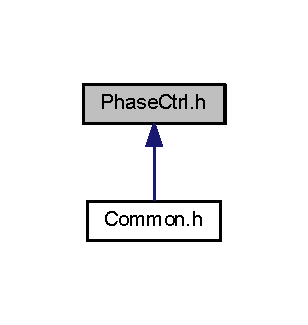
\includegraphics[width=148pt]{_phase_ctrl_8h__dep__incl}
\end{center}
\end{figure}
\subsection*{Functions}
\begin{DoxyCompactItemize}
\item 
void \hyperlink{_phase_ctrl_8h_a2aab767cee769a114c9e2ab25771e447}{pc\-Update} (void)
\end{DoxyCompactItemize}
\subsection*{Variables}
\begin{DoxyCompactItemize}
\item 
volatile int32 $\ast$ \hyperlink{_phase_ctrl_8h_ac286d0874ebba5141e36971f4a7f106e}{P\-H\-A\-S\-E\-\_\-\-C\-T\-R\-L\-\_\-\-In}
\end{DoxyCompactItemize}


\subsection{Detailed Description}
Signal generator phase (A\-C\-F\-B\-P\-H\-A\-S\-E) control function. \begin{DoxyWarning}{Warning}
This file is included by the file I\-S\-R.\-asm and thus any dependencies this file has should also be included there (e.\-g. Peripheral\-Header\-Includes.\-h). 
\end{DoxyWarning}


\subsection{Function Documentation}
\hypertarget{_phase_ctrl_8h_a2aab767cee769a114c9e2ab25771e447}{\index{Phase\-Ctrl.\-h@{Phase\-Ctrl.\-h}!pc\-Update@{pc\-Update}}
\index{pc\-Update@{pc\-Update}!PhaseCtrl.h@{Phase\-Ctrl.\-h}}
\subsubsection[{pc\-Update}]{\setlength{\rightskip}{0pt plus 5cm}void pc\-Update (
\begin{DoxyParamCaption}
\item[{void}]{}
\end{DoxyParamCaption}
)}}\label{_phase_ctrl_8h_a2aab767cee769a114c9e2ab25771e447}
Updates G\-P\-I\-O19 based on state of $\ast$\-P\-H\-A\-S\-E\-\_\-\-C\-T\-R\-L\-\_\-\-In terminal. Expects 0 (G\-P\-I\-O19 set) or non-\/zero (G\-P\-I\-O19 cleared). This is generally called by the D\-P\-L\-\_\-\-I\-S\-R.\-asm 

\subsection{Variable Documentation}
\hypertarget{_phase_ctrl_8h_ac286d0874ebba5141e36971f4a7f106e}{\index{Phase\-Ctrl.\-h@{Phase\-Ctrl.\-h}!P\-H\-A\-S\-E\-\_\-\-C\-T\-R\-L\-\_\-\-In@{P\-H\-A\-S\-E\-\_\-\-C\-T\-R\-L\-\_\-\-In}}
\index{P\-H\-A\-S\-E\-\_\-\-C\-T\-R\-L\-\_\-\-In@{P\-H\-A\-S\-E\-\_\-\-C\-T\-R\-L\-\_\-\-In}!PhaseCtrl.h@{Phase\-Ctrl.\-h}}
\subsubsection[{P\-H\-A\-S\-E\-\_\-\-C\-T\-R\-L\-\_\-\-In}]{\setlength{\rightskip}{0pt plus 5cm}volatile int32$\ast$ P\-H\-A\-S\-E\-\_\-\-C\-T\-R\-L\-\_\-\-In}}\label{_phase_ctrl_8h_ac286d0874ebba5141e36971f4a7f106e}
Phase control module signal input terminal. 
\hypertarget{_pwm_8h}{\section{Pwm.\-h File Reference}
\label{_pwm_8h}\index{Pwm.\-h@{Pwm.\-h}}
}


P\-W\-M and related functions.  


This graph shows which files directly or indirectly include this file\-:
\nopagebreak
\begin{figure}[H]
\begin{center}
\leavevmode
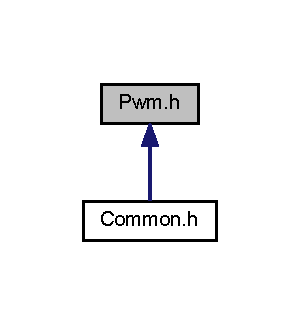
\includegraphics[width=144pt]{_pwm_8h__dep__incl}
\end{center}
\end{figure}
\subsection*{Macros}
\begin{DoxyCompactItemize}
\item 
\#define \hyperlink{_pwm_8h_af281425e62298bac2df0fbe8690a4844}{P\-E\-R\-I\-O\-D}~600
\end{DoxyCompactItemize}
\subsection*{Functions}
\begin{DoxyCompactItemize}
\item 
void \hyperlink{_pwm_8h_aced17503c602f9e71a2d101e956cce23}{pwm\-Tz\-Configure} (void)
\item 
void \hyperlink{_pwm_8h_a94a47896496e094f8ab54c1cb46da2e1}{pwm\-Rst\-Tz} (void)
\item 
void \hyperlink{_pwm_8h_acc68120fcdfa36145370c31a61eb23a7}{pwm\-Macro\-Configure} (void)
\item 
void \hyperlink{_pwm_8h_a358d8706acd0faf4e1cc705129be6548}{pwm\-Soc\-Configure} (void)
\item 
void \hyperlink{_pwm_8h_adfbaf2bb56a0c9fe6f54826499cb57de}{pwm\-D\-P\-L\-Trig\-Init} (void)
\item 
Uint16 \hyperlink{_pwm_8h_af82e2c1ff72afc3de42eb172ca925956}{pwm\-Set\-Freq} (Uint32 frq)
\item 
Uint16 \hyperlink{_pwm_8h_a79f203a5167440096f2ba270813b6db2}{pwm\-Get\-Freq} (Uint32 $\ast$frq\-Dest)
\end{DoxyCompactItemize}
\subsection*{Variables}
\begin{DoxyCompactItemize}
\item 
volatile int32 $\ast$ \hyperlink{_pwm_8h_a8a02650c6afb411447157faf0e90a7b2}{P\-W\-M\-D\-R\-V\-\_\-2ch\-\_\-\-Up\-Cnt\-\_\-\-Duty1\-A}
\item 
volatile int32 $\ast$ \hyperlink{_pwm_8h_a23767edc2ebfabc9336684185a4f2d84}{P\-W\-M\-D\-R\-V\-\_\-2ch\-\_\-\-Up\-Cnt\-\_\-\-Duty1\-B}
\item 
volatile int32 $\ast$ \hyperlink{_pwm_8h_acc76d5ffc745e63de05baa242bb3d16f}{P\-W\-M\-D\-R\-V\-\_\-2ch\-\_\-\-Up\-Cnt\-\_\-\-Duty2\-A}
\item 
volatile int32 $\ast$ \hyperlink{_pwm_8h_a3215b15b28994e0840d64200f09cbfb0}{P\-W\-M\-D\-R\-V\-\_\-2ch\-\_\-\-Up\-Cnt\-\_\-\-Duty2\-B}
\item 
volatile int32 $\ast$ \hyperlink{_pwm_8h_a86962b3c7a5a851d9ddce3301a9db727}{P\-W\-M\-D\-R\-V\-\_\-2ch\-\_\-\-Up\-Cnt\-\_\-\-Duty3\-A}
\item 
volatile int32 $\ast$ \hyperlink{_pwm_8h_a9550c95286e784256c9f12906ff5a407}{P\-W\-M\-D\-R\-V\-\_\-2ch\-\_\-\-Up\-Cnt\-\_\-\-Duty3\-B}
\end{DoxyCompactItemize}


\subsection{Detailed Description}
P\-W\-M and related functions. 

\subsection{Macro Definition Documentation}
\hypertarget{_pwm_8h_af281425e62298bac2df0fbe8690a4844}{\index{Pwm.\-h@{Pwm.\-h}!P\-E\-R\-I\-O\-D@{P\-E\-R\-I\-O\-D}}
\index{P\-E\-R\-I\-O\-D@{P\-E\-R\-I\-O\-D}!Pwm.h@{Pwm.\-h}}
\subsubsection[{P\-E\-R\-I\-O\-D}]{\setlength{\rightskip}{0pt plus 5cm}\#define P\-E\-R\-I\-O\-D~600}}\label{_pwm_8h_af281425e62298bac2df0fbe8690a4844}
Defines the initial P\-W\-M period setting = 60\-M\-Hz / 600 = 100. 

\subsection{Function Documentation}
\hypertarget{_pwm_8h_adfbaf2bb56a0c9fe6f54826499cb57de}{\index{Pwm.\-h@{Pwm.\-h}!pwm\-D\-P\-L\-Trig\-Init@{pwm\-D\-P\-L\-Trig\-Init}}
\index{pwm\-D\-P\-L\-Trig\-Init@{pwm\-D\-P\-L\-Trig\-Init}!Pwm.h@{Pwm.\-h}}
\subsubsection[{pwm\-D\-P\-L\-Trig\-Init}]{\setlength{\rightskip}{0pt plus 5cm}void pwm\-D\-P\-L\-Trig\-Init (
\begin{DoxyParamCaption}
\item[{void}]{}
\end{DoxyParamCaption}
)}}\label{_pwm_8h_adfbaf2bb56a0c9fe6f54826499cb57de}
Initialises and enables P\-W\-M1 (master) to trigger the D\-P\-L I\-S\-R. \hypertarget{_pwm_8h_a79f203a5167440096f2ba270813b6db2}{\index{Pwm.\-h@{Pwm.\-h}!pwm\-Get\-Freq@{pwm\-Get\-Freq}}
\index{pwm\-Get\-Freq@{pwm\-Get\-Freq}!Pwm.h@{Pwm.\-h}}
\subsubsection[{pwm\-Get\-Freq}]{\setlength{\rightskip}{0pt plus 5cm}Uint16 pwm\-Get\-Freq (
\begin{DoxyParamCaption}
\item[{Uint32 $\ast$}]{frq\-Dest}
\end{DoxyParamCaption}
)}}\label{_pwm_8h_a79f203a5167440096f2ba270813b6db2}
Queries the current P\-W\-M frequency setting. 
\begin{DoxyParams}[1]{Parameters}
\mbox{\tt out}  & {\em frq\-Dest} & Address of the memory location at which to place the query result (hertz). \\
\hline
\end{DoxyParams}
\begin{DoxyReturn}{Returns}
Error status. 
\end{DoxyReturn}
\hypertarget{_pwm_8h_acc68120fcdfa36145370c31a61eb23a7}{\index{Pwm.\-h@{Pwm.\-h}!pwm\-Macro\-Configure@{pwm\-Macro\-Configure}}
\index{pwm\-Macro\-Configure@{pwm\-Macro\-Configure}!Pwm.h@{Pwm.\-h}}
\subsubsection[{pwm\-Macro\-Configure}]{\setlength{\rightskip}{0pt plus 5cm}void pwm\-Macro\-Configure (
\begin{DoxyParamCaption}
\item[{void}]{}
\end{DoxyParamCaption}
)}}\label{_pwm_8h_acc68120fcdfa36145370c31a61eb23a7}
Configures each of the P\-W\-M macros for use. \hypertarget{_pwm_8h_a94a47896496e094f8ab54c1cb46da2e1}{\index{Pwm.\-h@{Pwm.\-h}!pwm\-Rst\-Tz@{pwm\-Rst\-Tz}}
\index{pwm\-Rst\-Tz@{pwm\-Rst\-Tz}!Pwm.h@{Pwm.\-h}}
\subsubsection[{pwm\-Rst\-Tz}]{\setlength{\rightskip}{0pt plus 5cm}void pwm\-Rst\-Tz (
\begin{DoxyParamCaption}
\item[{void}]{}
\end{DoxyParamCaption}
)}}\label{_pwm_8h_a94a47896496e094f8ab54c1cb46da2e1}
Resets the trip zone after a comparator event. \hypertarget{_pwm_8h_af82e2c1ff72afc3de42eb172ca925956}{\index{Pwm.\-h@{Pwm.\-h}!pwm\-Set\-Freq@{pwm\-Set\-Freq}}
\index{pwm\-Set\-Freq@{pwm\-Set\-Freq}!Pwm.h@{Pwm.\-h}}
\subsubsection[{pwm\-Set\-Freq}]{\setlength{\rightskip}{0pt plus 5cm}Uint16 pwm\-Set\-Freq (
\begin{DoxyParamCaption}
\item[{Uint32}]{frq}
\end{DoxyParamCaption}
)}}\label{_pwm_8h_af82e2c1ff72afc3de42eb172ca925956}
Sets the frequency of the P\-W\-Ms. 
\begin{DoxyParams}[1]{Parameters}
\mbox{\tt in}  & {\em frq} & Specifies the required frequency (hertz). \\
\hline
\end{DoxyParams}
\begin{DoxyReturn}{Returns}
Error status. 
\end{DoxyReturn}
\hypertarget{_pwm_8h_a358d8706acd0faf4e1cc705129be6548}{\index{Pwm.\-h@{Pwm.\-h}!pwm\-Soc\-Configure@{pwm\-Soc\-Configure}}
\index{pwm\-Soc\-Configure@{pwm\-Soc\-Configure}!Pwm.h@{Pwm.\-h}}
\subsubsection[{pwm\-Soc\-Configure}]{\setlength{\rightskip}{0pt plus 5cm}void pwm\-Soc\-Configure (
\begin{DoxyParamCaption}
\item[{void}]{}
\end{DoxyParamCaption}
)}}\label{_pwm_8h_a358d8706acd0faf4e1cc705129be6548}
Configures P\-W\-M1 (master) to generate A\-D\-C S\-O\-C start for A\-D\-C macro -\/ configure before initialisation. \hypertarget{_pwm_8h_aced17503c602f9e71a2d101e956cce23}{\index{Pwm.\-h@{Pwm.\-h}!pwm\-Tz\-Configure@{pwm\-Tz\-Configure}}
\index{pwm\-Tz\-Configure@{pwm\-Tz\-Configure}!Pwm.h@{Pwm.\-h}}
\subsubsection[{pwm\-Tz\-Configure}]{\setlength{\rightskip}{0pt plus 5cm}void pwm\-Tz\-Configure (
\begin{DoxyParamCaption}
\item[{void}]{}
\end{DoxyParamCaption}
)}}\label{_pwm_8h_aced17503c602f9e71a2d101e956cce23}
Configures P\-W\-M trip zones for use. Requires the comparator and D\-A\-C to be configured \begin{DoxySeeAlso}{See Also}
\hyperlink{_adc_8h}{adc.\-h} 
\end{DoxySeeAlso}


\subsection{Variable Documentation}
\hypertarget{_pwm_8h_a8a02650c6afb411447157faf0e90a7b2}{\index{Pwm.\-h@{Pwm.\-h}!P\-W\-M\-D\-R\-V\-\_\-2ch\-\_\-\-Up\-Cnt\-\_\-\-Duty1\-A@{P\-W\-M\-D\-R\-V\-\_\-2ch\-\_\-\-Up\-Cnt\-\_\-\-Duty1\-A}}
\index{P\-W\-M\-D\-R\-V\-\_\-2ch\-\_\-\-Up\-Cnt\-\_\-\-Duty1\-A@{P\-W\-M\-D\-R\-V\-\_\-2ch\-\_\-\-Up\-Cnt\-\_\-\-Duty1\-A}!Pwm.h@{Pwm.\-h}}
\subsubsection[{P\-W\-M\-D\-R\-V\-\_\-2ch\-\_\-\-Up\-Cnt\-\_\-\-Duty1\-A}]{\setlength{\rightskip}{0pt plus 5cm}volatile int32$\ast$ P\-W\-M\-D\-R\-V\-\_\-2ch\-\_\-\-Up\-Cnt\-\_\-\-Duty1\-A}}\label{_pwm_8h_a8a02650c6afb411447157faf0e90a7b2}
Channel 0 P\-W\-M terminal pointer. \hypertarget{_pwm_8h_a23767edc2ebfabc9336684185a4f2d84}{\index{Pwm.\-h@{Pwm.\-h}!P\-W\-M\-D\-R\-V\-\_\-2ch\-\_\-\-Up\-Cnt\-\_\-\-Duty1\-B@{P\-W\-M\-D\-R\-V\-\_\-2ch\-\_\-\-Up\-Cnt\-\_\-\-Duty1\-B}}
\index{P\-W\-M\-D\-R\-V\-\_\-2ch\-\_\-\-Up\-Cnt\-\_\-\-Duty1\-B@{P\-W\-M\-D\-R\-V\-\_\-2ch\-\_\-\-Up\-Cnt\-\_\-\-Duty1\-B}!Pwm.h@{Pwm.\-h}}
\subsubsection[{P\-W\-M\-D\-R\-V\-\_\-2ch\-\_\-\-Up\-Cnt\-\_\-\-Duty1\-B}]{\setlength{\rightskip}{0pt plus 5cm}volatile int32$\ast$ P\-W\-M\-D\-R\-V\-\_\-2ch\-\_\-\-Up\-Cnt\-\_\-\-Duty1\-B}}\label{_pwm_8h_a23767edc2ebfabc9336684185a4f2d84}
Channel 1 P\-W\-M terminal pointers. \hypertarget{_pwm_8h_acc76d5ffc745e63de05baa242bb3d16f}{\index{Pwm.\-h@{Pwm.\-h}!P\-W\-M\-D\-R\-V\-\_\-2ch\-\_\-\-Up\-Cnt\-\_\-\-Duty2\-A@{P\-W\-M\-D\-R\-V\-\_\-2ch\-\_\-\-Up\-Cnt\-\_\-\-Duty2\-A}}
\index{P\-W\-M\-D\-R\-V\-\_\-2ch\-\_\-\-Up\-Cnt\-\_\-\-Duty2\-A@{P\-W\-M\-D\-R\-V\-\_\-2ch\-\_\-\-Up\-Cnt\-\_\-\-Duty2\-A}!Pwm.h@{Pwm.\-h}}
\subsubsection[{P\-W\-M\-D\-R\-V\-\_\-2ch\-\_\-\-Up\-Cnt\-\_\-\-Duty2\-A}]{\setlength{\rightskip}{0pt plus 5cm}volatile int32$\ast$ P\-W\-M\-D\-R\-V\-\_\-2ch\-\_\-\-Up\-Cnt\-\_\-\-Duty2\-A}}\label{_pwm_8h_acc76d5ffc745e63de05baa242bb3d16f}
Channel 2 P\-W\-M terminal pointer. \hypertarget{_pwm_8h_a3215b15b28994e0840d64200f09cbfb0}{\index{Pwm.\-h@{Pwm.\-h}!P\-W\-M\-D\-R\-V\-\_\-2ch\-\_\-\-Up\-Cnt\-\_\-\-Duty2\-B@{P\-W\-M\-D\-R\-V\-\_\-2ch\-\_\-\-Up\-Cnt\-\_\-\-Duty2\-B}}
\index{P\-W\-M\-D\-R\-V\-\_\-2ch\-\_\-\-Up\-Cnt\-\_\-\-Duty2\-B@{P\-W\-M\-D\-R\-V\-\_\-2ch\-\_\-\-Up\-Cnt\-\_\-\-Duty2\-B}!Pwm.h@{Pwm.\-h}}
\subsubsection[{P\-W\-M\-D\-R\-V\-\_\-2ch\-\_\-\-Up\-Cnt\-\_\-\-Duty2\-B}]{\setlength{\rightskip}{0pt plus 5cm}volatile int32$\ast$ P\-W\-M\-D\-R\-V\-\_\-2ch\-\_\-\-Up\-Cnt\-\_\-\-Duty2\-B}}\label{_pwm_8h_a3215b15b28994e0840d64200f09cbfb0}
Channel 3 P\-W\-M terminal pointer. \hypertarget{_pwm_8h_a86962b3c7a5a851d9ddce3301a9db727}{\index{Pwm.\-h@{Pwm.\-h}!P\-W\-M\-D\-R\-V\-\_\-2ch\-\_\-\-Up\-Cnt\-\_\-\-Duty3\-A@{P\-W\-M\-D\-R\-V\-\_\-2ch\-\_\-\-Up\-Cnt\-\_\-\-Duty3\-A}}
\index{P\-W\-M\-D\-R\-V\-\_\-2ch\-\_\-\-Up\-Cnt\-\_\-\-Duty3\-A@{P\-W\-M\-D\-R\-V\-\_\-2ch\-\_\-\-Up\-Cnt\-\_\-\-Duty3\-A}!Pwm.h@{Pwm.\-h}}
\subsubsection[{P\-W\-M\-D\-R\-V\-\_\-2ch\-\_\-\-Up\-Cnt\-\_\-\-Duty3\-A}]{\setlength{\rightskip}{0pt plus 5cm}volatile int32$\ast$ P\-W\-M\-D\-R\-V\-\_\-2ch\-\_\-\-Up\-Cnt\-\_\-\-Duty3\-A}}\label{_pwm_8h_a86962b3c7a5a851d9ddce3301a9db727}
Interboost P\-W\-M terminal pointer. \hypertarget{_pwm_8h_a9550c95286e784256c9f12906ff5a407}{\index{Pwm.\-h@{Pwm.\-h}!P\-W\-M\-D\-R\-V\-\_\-2ch\-\_\-\-Up\-Cnt\-\_\-\-Duty3\-B@{P\-W\-M\-D\-R\-V\-\_\-2ch\-\_\-\-Up\-Cnt\-\_\-\-Duty3\-B}}
\index{P\-W\-M\-D\-R\-V\-\_\-2ch\-\_\-\-Up\-Cnt\-\_\-\-Duty3\-B@{P\-W\-M\-D\-R\-V\-\_\-2ch\-\_\-\-Up\-Cnt\-\_\-\-Duty3\-B}!Pwm.h@{Pwm.\-h}}
\subsubsection[{P\-W\-M\-D\-R\-V\-\_\-2ch\-\_\-\-Up\-Cnt\-\_\-\-Duty3\-B}]{\setlength{\rightskip}{0pt plus 5cm}volatile int32$\ast$ P\-W\-M\-D\-R\-V\-\_\-2ch\-\_\-\-Up\-Cnt\-\_\-\-Duty3\-B}}\label{_pwm_8h_a9550c95286e784256c9f12906ff5a407}
A\-C stage P\-W\-M terminal pointer. 
\hypertarget{_sci_8h}{\section{Sci.\-h File Reference}
\label{_sci_8h}\index{Sci.\-h@{Sci.\-h}}
}


S\-C\-I communications functions.  


This graph shows which files directly or indirectly include this file\-:\nopagebreak
\begin{figure}[H]
\begin{center}
\leavevmode
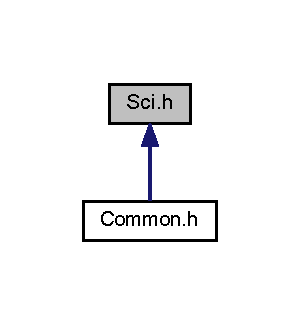
\includegraphics[width=144pt]{_sci_8h__dep__incl}
\end{center}
\end{figure}
\subsection*{Macros}
\begin{DoxyCompactItemize}
\item 
\#define \hyperlink{_sci_8h_a0e4c420431b12616b61e9f3a28f07e4d}{S\-C\-I\-B\-A\-U\-D\-\_\-\-M\-I\-N}~29
\item 
\#define \hyperlink{_sci_8h_a5733933fffc18dbcb8bc9404e80bc493}{S\-C\-I\-F\-F\-R\-X\-\_\-\-I\-N\-T\-\_\-\-L\-V\-L}~1
\item 
\#define \hyperlink{_sci_8h_a5340c9de55b8e5c65ef801d2dcabffd7}{S\-C\-I\-F\-F\-T\-X\-\_\-\-I\-N\-T\-\_\-\-L\-V\-L}~0
\item 
\#define \hyperlink{_sci_8h_af0368b1c16e194a32bf4ce09eb937930}{S\-C\-I\-F\-F\-T\-X\-\_\-\-F\-I\-L\-L\-\_\-\-L\-V\-L}~4
\end{DoxyCompactItemize}
\subsection*{Functions}
\begin{DoxyCompactItemize}
\item 
Uint16 \hyperlink{_sci_8h_a1f05b9c5226c73b67c1d6c3bf7f80b52}{sci\-Init} (Uint32 baud)
\item 
void \hyperlink{_sci_8h_a941bdbf3e64ac5f4492a7f7c5936b445}{sci\-Tx} (void)
\end{DoxyCompactItemize}


\subsection{Detailed Description}
S\-C\-I communications functions. \begin{DoxyParagraph}{}
On the T\-I C2000 Launch\-Pad X\-L\-: \begin{TabularC}{3}
\hline
\rowcolor{lightgray}\PBS\centering {\bf Function}&\PBS\centering {\bf G\-P\-I\-O }&\PBS\centering {\bf P\-C\-B Pin  }\\\cline{1-3}
\PBS\centering S\-C\-I\-\_\-\-R\-X &\PBS\centering G\-P\-I\-O28&\PBS\centering J1-\/3 \\\cline{1-3}
\PBS\centering S\-C\-I\-\_\-\-T\-X &\PBS\centering G\-P\-I\-O29&\PBS\centering J1-\/4 \\\cline{1-3}
\end{TabularC}

\end{DoxyParagraph}
\begin{DoxyWarning}{Warning}
On the T\-I C2000 Launch\-Pad X\-L the switch 4 (S4) should be in the O\-F\-F position to communicate with devices other than the on-\/board U\-S\-B controller. 
\end{DoxyWarning}


\subsection{Macro Definition Documentation}
\hypertarget{_sci_8h_a0e4c420431b12616b61e9f3a28f07e4d}{\index{Sci.\-h@{Sci.\-h}!S\-C\-I\-B\-A\-U\-D\-\_\-\-M\-I\-N@{S\-C\-I\-B\-A\-U\-D\-\_\-\-M\-I\-N}}
\index{S\-C\-I\-B\-A\-U\-D\-\_\-\-M\-I\-N@{S\-C\-I\-B\-A\-U\-D\-\_\-\-M\-I\-N}!Sci.h@{Sci.\-h}}
\subsubsection[{S\-C\-I\-B\-A\-U\-D\-\_\-\-M\-I\-N}]{\setlength{\rightskip}{0pt plus 5cm}\#define S\-C\-I\-B\-A\-U\-D\-\_\-\-M\-I\-N~29}}\label{_sci_8h_a0e4c420431b12616b61e9f3a28f07e4d}
Minimum allowable value of S\-C\-I Baud. \hypertarget{_sci_8h_a5733933fffc18dbcb8bc9404e80bc493}{\index{Sci.\-h@{Sci.\-h}!S\-C\-I\-F\-F\-R\-X\-\_\-\-I\-N\-T\-\_\-\-L\-V\-L@{S\-C\-I\-F\-F\-R\-X\-\_\-\-I\-N\-T\-\_\-\-L\-V\-L}}
\index{S\-C\-I\-F\-F\-R\-X\-\_\-\-I\-N\-T\-\_\-\-L\-V\-L@{S\-C\-I\-F\-F\-R\-X\-\_\-\-I\-N\-T\-\_\-\-L\-V\-L}!Sci.h@{Sci.\-h}}
\subsubsection[{S\-C\-I\-F\-F\-R\-X\-\_\-\-I\-N\-T\-\_\-\-L\-V\-L}]{\setlength{\rightskip}{0pt plus 5cm}\#define S\-C\-I\-F\-F\-R\-X\-\_\-\-I\-N\-T\-\_\-\-L\-V\-L~1}}\label{_sci_8h_a5733933fffc18dbcb8bc9404e80bc493}
Interrupt level for receiving F\-I\-F\-O. \hypertarget{_sci_8h_af0368b1c16e194a32bf4ce09eb937930}{\index{Sci.\-h@{Sci.\-h}!S\-C\-I\-F\-F\-T\-X\-\_\-\-F\-I\-L\-L\-\_\-\-L\-V\-L@{S\-C\-I\-F\-F\-T\-X\-\_\-\-F\-I\-L\-L\-\_\-\-L\-V\-L}}
\index{S\-C\-I\-F\-F\-T\-X\-\_\-\-F\-I\-L\-L\-\_\-\-L\-V\-L@{S\-C\-I\-F\-F\-T\-X\-\_\-\-F\-I\-L\-L\-\_\-\-L\-V\-L}!Sci.h@{Sci.\-h}}
\subsubsection[{S\-C\-I\-F\-F\-T\-X\-\_\-\-F\-I\-L\-L\-\_\-\-L\-V\-L}]{\setlength{\rightskip}{0pt plus 5cm}\#define S\-C\-I\-F\-F\-T\-X\-\_\-\-F\-I\-L\-L\-\_\-\-L\-V\-L~4}}\label{_sci_8h_af0368b1c16e194a32bf4ce09eb937930}
Fill level for transmission F\-I\-F\-O. \hypertarget{_sci_8h_a5340c9de55b8e5c65ef801d2dcabffd7}{\index{Sci.\-h@{Sci.\-h}!S\-C\-I\-F\-F\-T\-X\-\_\-\-I\-N\-T\-\_\-\-L\-V\-L@{S\-C\-I\-F\-F\-T\-X\-\_\-\-I\-N\-T\-\_\-\-L\-V\-L}}
\index{S\-C\-I\-F\-F\-T\-X\-\_\-\-I\-N\-T\-\_\-\-L\-V\-L@{S\-C\-I\-F\-F\-T\-X\-\_\-\-I\-N\-T\-\_\-\-L\-V\-L}!Sci.h@{Sci.\-h}}
\subsubsection[{S\-C\-I\-F\-F\-T\-X\-\_\-\-I\-N\-T\-\_\-\-L\-V\-L}]{\setlength{\rightskip}{0pt plus 5cm}\#define S\-C\-I\-F\-F\-T\-X\-\_\-\-I\-N\-T\-\_\-\-L\-V\-L~0}}\label{_sci_8h_a5340c9de55b8e5c65ef801d2dcabffd7}
Interrupt level for transmission F\-I\-F\-O. 

\subsection{Function Documentation}
\hypertarget{_sci_8h_a1f05b9c5226c73b67c1d6c3bf7f80b52}{\index{Sci.\-h@{Sci.\-h}!sci\-Init@{sci\-Init}}
\index{sci\-Init@{sci\-Init}!Sci.h@{Sci.\-h}}
\subsubsection[{sci\-Init}]{\setlength{\rightskip}{0pt plus 5cm}Uint16 sci\-Init (
\begin{DoxyParamCaption}
\item[{Uint32}]{baud}
\end{DoxyParamCaption}
)}}\label{_sci_8h_a1f05b9c5226c73b67c1d6c3bf7f80b52}
Initialises the S\-C\-I(\-A) peripheral and relate interrupts. 
\begin{DoxyParams}[1]{Parameters}
\mbox{\tt in}  & {\em baud} & The baud rate that the S\-C\-I should use minimum value is set by S\-C\-I\-B\-A\-U\-D\-\_\-\-M\-I\-N. \\
\hline
\end{DoxyParams}
\begin{DoxyReturn}{Returns}
Error status.
\end{DoxyReturn}
\begin{DoxyWarning}{Warning}
This function M\-U\-S\-T be called before any other S\-C\-I(\-A) function. 

This function will clear any values placed in the associated S\-C\-I(\-A) registers prior to calling. 
\end{DoxyWarning}
\hypertarget{_sci_8h_a941bdbf3e64ac5f4492a7f7c5936b445}{\index{Sci.\-h@{Sci.\-h}!sci\-Tx@{sci\-Tx}}
\index{sci\-Tx@{sci\-Tx}!Sci.h@{Sci.\-h}}
\subsubsection[{sci\-Tx}]{\setlength{\rightskip}{0pt plus 5cm}void sci\-Tx (
\begin{DoxyParamCaption}
\item[{void}]{}
\end{DoxyParamCaption}
)}}\label{_sci_8h_a941bdbf3e64ac5f4492a7f7c5936b445}
Transmits whatever data is on the S\-C\-P\-I output queue. 
\hypertarget{_s_c_p_i__specific_cmds_8h}{\section{S\-C\-P\-I\-\_\-specific\-Cmds.\-h File Reference}
\label{_s_c_p_i__specific_cmds_8h}\index{S\-C\-P\-I\-\_\-specific\-Cmds.\-h@{S\-C\-P\-I\-\_\-specific\-Cmds.\-h}}
}
This graph shows which files directly or indirectly include this file\-:\nopagebreak
\begin{figure}[H]
\begin{center}
\leavevmode
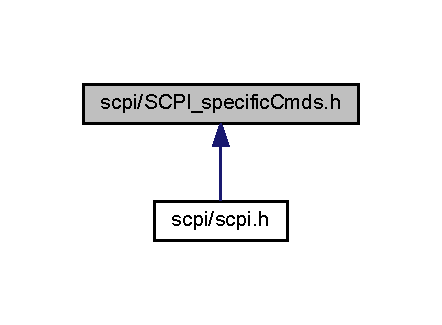
\includegraphics[width=190pt]{_s_c_p_i__specific_cmds_8h__dep__incl}
\end{center}
\end{figure}


\subsection{Detailed Description}
This file includes the functions for registering the application specific commands and the related callback functions

These commands and their associated callback functions can be edited to suit the application in use, though they should follow the guidelines and conventions laid out in I\-E\-E\-E 488.\-2-\/1992 and S\-C\-P\-I-\/1999

Please follow the information in the parser documentation and the file S\-C\-P\-I\-\_\-specific\-Cmds.\-c on how to add or change message headers, commands and parameters

To register a new command device specific tree node, add a register\-Child() call to the function register\-Specific\-Commands() with the form \char`\"{}err += register\-Child(\-C\-H\-I\-L\-D\-\_\-\-L\-O\-N\-G\-\_\-\-N\-A\-M\-E, P\-A\-R\-E\-N\-T\-\_\-\-S\-H\-O\-R\-T\-\_\-\-N\-A\-M\-E,
\-B\-O\-O\-L\-\_\-\-I\-S\-\_\-\-H\-E\-A\-D\-E\-R\-\_\-\-O\-N\-L\-Y, B\-O\-O\-L\-\_\-\-I\-S\-\_\-\-Q\-U\-E\-R\-Y, C\-A\-L\-L\-B\-A\-C\-K\-\_\-\-H\-A\-N\-D\-L\-E);\char`\"{}, where\-:
\begin{DoxyItemize}
\item C\-H\-I\-L\-D\-\_\-\-L\-O\-N\-G\-\_\-\-N\-A\-M\-E is the long form of the name of the child node to be registered.
\item P\-A\-R\-E\-N\-T\-\_\-\-S\-H\-O\-R\-T\-\_\-\-N\-A\-M\-E is the short form of the name of the parent of the child node to be registered. This must be an already existing node.
\item B\-O\-O\-L\-\_\-\-I\-S\-\_\-\-H\-E\-A\-D\-E\-R\-\_\-\-O\-N\-L\-Y is a boolean value that indicates if the node being registered is a header only (i.\-e. is not a command) or not.
\item B\-O\-O\-L\-\_\-\-I\-S\-\_\-\-Q\-U\-E\-R\-Y is a boolean value that indicates if the node being registered my be queried or not.
\item C\-A\-L\-L\-B\-A\-C\-K\-\_\-\-H\-A\-N\-D\-L\-E is a pointer to the function to be associated with this child if it is a command, or N\-U\-L\-L if it is a header only.
\end{DoxyItemize}

For further information on the operation of register\-Child() please see the function description.

All string literals M\-U\-S\-T be in upper case and enclosed in quotation marks.

Node long and short names must conform to the standard as outlined by S\-C\-P\-I-\/99 in 6.\-2.\-1

All tree nodes are children of at least \char`\"{}\-R\-O\-O\-T\char`\"{}. Changes to the number of node registered should be reflected by the user in the number defined for T\-R\-E\-E\-\_\-\-C\-H\-I\-L\-D\-\_\-\-L\-I\-M\-I\-T in scpi.\-h 
\hypertarget{_settings_8h}{\section{Settings.\-h File Reference}
\label{_settings_8h}\index{Settings.\-h@{Settings.\-h}}
}


Major build definitions and settings for the project.  


This graph shows which files directly or indirectly include this file\-:\nopagebreak
\begin{figure}[H]
\begin{center}
\leavevmode
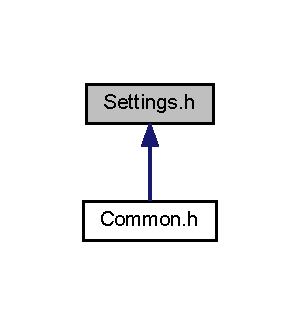
\includegraphics[width=144pt]{_settings_8h__dep__incl}
\end{center}
\end{figure}
\subsection*{Macros}
\begin{DoxyCompactItemize}
\item 
\#define \hyperlink{_settings_8h_abf493281a7e64fe88660c38753e18d56}{I\-N\-C\-R\-\_\-\-B\-U\-I\-L\-D}~2
\item 
\#define \hyperlink{_settings_8h_ad72dbcf6d0153db1b8d8a58001feed83}{D\-E\-B\-U\-G}
\item 
\#define \hyperlink{_settings_8h_a67e401b420276bcc62502f8f81a4bfcb}{U\-S\-E\-\_\-\-P\-I\-D}
\item 
\#define \hyperlink{_settings_8h_a1381ac724d85872e7c3e388fd817b624}{T\-E\-S\-T\-\_\-\-T\-Z}
\item 
\#define \hyperlink{_settings_8h_a3c2e957a61cfa19e31e8477fe3aacab8}{V\-S\-S\-A}~0l
\item 
\#define \hyperlink{_settings_8h_a511faa1530ba984d340a884a97e6a80a}{V\-M\-I\-D\-\_\-\-R1}~540.\-0
\item 
\#define \hyperlink{_settings_8h_a86d7f47e3c125143c21e1ca2836eb4ab}{V\-M\-I\-D\-\_\-\-R2}~4.\-3
\item 
\#define \hyperlink{_settings_8h_a67fad1f78c49251e39fa6f1d5ff43e9e}{V\-A\-C\-\_\-\-R1}~540.\-0
\item 
\#define \hyperlink{_settings_8h_a087778c4195e73f588e5c3cf7d9e9206}{V\-A\-C\-\_\-\-R2}~4.\-3
\item 
\#define \hyperlink{_settings_8h_a69b2e41c3deaae85991311202c4a1a14}{N\-U\-M\-\_\-\-I\-C\-T\-R\-L\-\_\-\-C\-H\-N\-L\-S}~5
\item 
\#define \hyperlink{_settings_8h_a42a316162edffd07a32e68a889760c06}{N\-U\-M\-\_\-\-V\-C\-T\-R\-L\-\_\-\-C\-H\-N\-L\-S}~2
\item 
\#define \hyperlink{_settings_8h_afe433b138bb71d8d26b6e0907e656d1b}{N\-U\-M\-\_\-\-C\-H\-N\-L\-S}~\hyperlink{_settings_8h_a69b2e41c3deaae85991311202c4a1a14}{N\-U\-M\-\_\-\-I\-C\-T\-R\-L\-\_\-\-C\-H\-N\-L\-S} + \hyperlink{_settings_8h_a42a316162edffd07a32e68a889760c06}{N\-U\-M\-\_\-\-V\-C\-T\-R\-L\-\_\-\-C\-H\-N\-L\-S}
\item 
\#define \hyperlink{_settings_8h_abc63ab2a8e7782de38a5dbdfc33da717}{S\-Q\-R\-T\-\_\-2}~1.\-41429
\item 
\#define \hyperlink{_settings_8h_ae468f418f2e6410dfcfeb58bcbbde516}{R\-E\-C\-P\-\_\-\-S\-Q\-R\-T\-\_\-2}~0.\-70711
\item 
\#define \hyperlink{_settings_8h_a2d52976aedaedf74a90019a689170620}{V\-D\-D\-A}~3300l
\item 
\#define \hyperlink{_settings_8h_aa010c11f88da0f9a48a7dfd810412d5d}{u\-Sec100}~6000
\end{DoxyCompactItemize}
{\bf }\par
\begin{DoxyCompactItemize}
\item 
\#define \hyperlink{_settings_8h_a5f4c019658ca5a8eff4bfc3d96d489a0}{C\-H\-A\-N\-N\-E\-L\-\_\-\-O\-O\-B}~0x10
\item 
\#define \hyperlink{_settings_8h_a055087c0064c322a05e443b47479bfe1}{V\-A\-L\-U\-E\-\_\-\-O\-O\-B}~0x11
\item 
\#define \hyperlink{_settings_8h_a42d97deed6614a0b5b0aee655055b43a}{O\-C\-P\-\_\-\-T\-R\-I\-P}~0x12
\item 
\#define \hyperlink{_settings_8h_ac330c784fd08c389f8649ac8e34d29e8}{O\-V\-P\-\_\-\-T\-R\-I\-P}~0x13
\item 
\#define \hyperlink{_settings_8h_a5815c03ac63c324e326a148e247f24a1}{O\-T\-P\-\_\-\-T\-R\-I\-P}~0x14
\item 
\#define \hyperlink{_settings_8h_aec1cab1af7dceb601fa90842135a4f65}{I2\-C\-\_\-\-R\-E\-A\-D\-\_\-\-W\-R\-O\-N\-G\-\_\-\-M\-S\-G}~0x20
\item 
\#define \hyperlink{_settings_8h_ac6997f1781d1d9047bd556dd5152795b}{I2\-C\-\_\-\-W\-R\-I\-T\-E\-\_\-\-W\-R\-O\-N\-G\-\_\-\-M\-S\-G}~0x21
\item 
\#define \hyperlink{_settings_8h_af623f6210c2ce545f939ec061fc533b0}{I2\-C\-\_\-\-S\-T\-P\-\_\-\-N\-O\-T\-\_\-\-R\-E\-A\-D\-Y}~0x22
\item 
\#define \hyperlink{_settings_8h_ad3082827214b064d5b8289acaeb9ad20}{I2\-C\-\_\-\-B\-U\-S\-\_\-\-B\-U\-S\-Y}~0x23
\item 
\#define \hyperlink{_settings_8h_a8e605ae1b9fc359d203b90cb9f8a090e}{I2\-C\-\_\-\-I\-N\-V\-A\-L\-I\-D\-\_\-\-I\-S\-R\-C}~0x24
\end{DoxyCompactItemize}



\subsection{Detailed Description}
Major build definitions and settings for the project. \begin{DoxyWarning}{Warning}
This file is included and referenced by I\-S\-R.\-asm, main() and \hyperlink{_macro_nets_8h_a06d36d85b8d9d27cfc6674244ef1e603}{mn\-Connect\-Nets()}.

When changes are made to this file please use rebuild all. 
\end{DoxyWarning}


\subsection{Macro Definition Documentation}
\hypertarget{_settings_8h_a5f4c019658ca5a8eff4bfc3d96d489a0}{\index{Settings.\-h@{Settings.\-h}!C\-H\-A\-N\-N\-E\-L\-\_\-\-O\-O\-B@{C\-H\-A\-N\-N\-E\-L\-\_\-\-O\-O\-B}}
\index{C\-H\-A\-N\-N\-E\-L\-\_\-\-O\-O\-B@{C\-H\-A\-N\-N\-E\-L\-\_\-\-O\-O\-B}!Settings.h@{Settings.\-h}}
\subsubsection[{C\-H\-A\-N\-N\-E\-L\-\_\-\-O\-O\-B}]{\setlength{\rightskip}{0pt plus 5cm}\#define C\-H\-A\-N\-N\-E\-L\-\_\-\-O\-O\-B~0x10}}\label{_settings_8h_a5f4c019658ca5a8eff4bfc3d96d489a0}
Channel out of bounds error code. \hypertarget{_settings_8h_ad72dbcf6d0153db1b8d8a58001feed83}{\index{Settings.\-h@{Settings.\-h}!D\-E\-B\-U\-G@{D\-E\-B\-U\-G}}
\index{D\-E\-B\-U\-G@{D\-E\-B\-U\-G}!Settings.h@{Settings.\-h}}
\subsubsection[{D\-E\-B\-U\-G}]{\setlength{\rightskip}{0pt plus 5cm}\#define D\-E\-B\-U\-G}}\label{_settings_8h_ad72dbcf6d0153db1b8d8a58001feed83}
Includes and makes functions and variables public that are used only for debugging purposes. \hypertarget{_settings_8h_ad3082827214b064d5b8289acaeb9ad20}{\index{Settings.\-h@{Settings.\-h}!I2\-C\-\_\-\-B\-U\-S\-\_\-\-B\-U\-S\-Y@{I2\-C\-\_\-\-B\-U\-S\-\_\-\-B\-U\-S\-Y}}
\index{I2\-C\-\_\-\-B\-U\-S\-\_\-\-B\-U\-S\-Y@{I2\-C\-\_\-\-B\-U\-S\-\_\-\-B\-U\-S\-Y}!Settings.h@{Settings.\-h}}
\subsubsection[{I2\-C\-\_\-\-B\-U\-S\-\_\-\-B\-U\-S\-Y}]{\setlength{\rightskip}{0pt plus 5cm}\#define I2\-C\-\_\-\-B\-U\-S\-\_\-\-B\-U\-S\-Y~0x23}}\label{_settings_8h_ad3082827214b064d5b8289acaeb9ad20}
I2\-C bus already busy error code. \hypertarget{_settings_8h_a8e605ae1b9fc359d203b90cb9f8a090e}{\index{Settings.\-h@{Settings.\-h}!I2\-C\-\_\-\-I\-N\-V\-A\-L\-I\-D\-\_\-\-I\-S\-R\-C@{I2\-C\-\_\-\-I\-N\-V\-A\-L\-I\-D\-\_\-\-I\-S\-R\-C}}
\index{I2\-C\-\_\-\-I\-N\-V\-A\-L\-I\-D\-\_\-\-I\-S\-R\-C@{I2\-C\-\_\-\-I\-N\-V\-A\-L\-I\-D\-\_\-\-I\-S\-R\-C}!Settings.h@{Settings.\-h}}
\subsubsection[{I2\-C\-\_\-\-I\-N\-V\-A\-L\-I\-D\-\_\-\-I\-S\-R\-C}]{\setlength{\rightskip}{0pt plus 5cm}\#define I2\-C\-\_\-\-I\-N\-V\-A\-L\-I\-D\-\_\-\-I\-S\-R\-C~0x24}}\label{_settings_8h_a8e605ae1b9fc359d203b90cb9f8a090e}
Invalid I2\-C interrupt source error code. \hypertarget{_settings_8h_aec1cab1af7dceb601fa90842135a4f65}{\index{Settings.\-h@{Settings.\-h}!I2\-C\-\_\-\-R\-E\-A\-D\-\_\-\-W\-R\-O\-N\-G\-\_\-\-M\-S\-G@{I2\-C\-\_\-\-R\-E\-A\-D\-\_\-\-W\-R\-O\-N\-G\-\_\-\-M\-S\-G}}
\index{I2\-C\-\_\-\-R\-E\-A\-D\-\_\-\-W\-R\-O\-N\-G\-\_\-\-M\-S\-G@{I2\-C\-\_\-\-R\-E\-A\-D\-\_\-\-W\-R\-O\-N\-G\-\_\-\-M\-S\-G}!Settings.h@{Settings.\-h}}
\subsubsection[{I2\-C\-\_\-\-R\-E\-A\-D\-\_\-\-W\-R\-O\-N\-G\-\_\-\-M\-S\-G}]{\setlength{\rightskip}{0pt plus 5cm}\#define I2\-C\-\_\-\-R\-E\-A\-D\-\_\-\-W\-R\-O\-N\-G\-\_\-\-M\-S\-G~0x20}}\label{_settings_8h_aec1cab1af7dceb601fa90842135a4f65}
Incorrect type I2\-C message read error code. \hypertarget{_settings_8h_af623f6210c2ce545f939ec061fc533b0}{\index{Settings.\-h@{Settings.\-h}!I2\-C\-\_\-\-S\-T\-P\-\_\-\-N\-O\-T\-\_\-\-R\-E\-A\-D\-Y@{I2\-C\-\_\-\-S\-T\-P\-\_\-\-N\-O\-T\-\_\-\-R\-E\-A\-D\-Y}}
\index{I2\-C\-\_\-\-S\-T\-P\-\_\-\-N\-O\-T\-\_\-\-R\-E\-A\-D\-Y@{I2\-C\-\_\-\-S\-T\-P\-\_\-\-N\-O\-T\-\_\-\-R\-E\-A\-D\-Y}!Settings.h@{Settings.\-h}}
\subsubsection[{I2\-C\-\_\-\-S\-T\-P\-\_\-\-N\-O\-T\-\_\-\-R\-E\-A\-D\-Y}]{\setlength{\rightskip}{0pt plus 5cm}\#define I2\-C\-\_\-\-S\-T\-P\-\_\-\-N\-O\-T\-\_\-\-R\-E\-A\-D\-Y~0x22}}\label{_settings_8h_af623f6210c2ce545f939ec061fc533b0}
I2\-C stop bit was not yet received error code. \hypertarget{_settings_8h_ac6997f1781d1d9047bd556dd5152795b}{\index{Settings.\-h@{Settings.\-h}!I2\-C\-\_\-\-W\-R\-I\-T\-E\-\_\-\-W\-R\-O\-N\-G\-\_\-\-M\-S\-G@{I2\-C\-\_\-\-W\-R\-I\-T\-E\-\_\-\-W\-R\-O\-N\-G\-\_\-\-M\-S\-G}}
\index{I2\-C\-\_\-\-W\-R\-I\-T\-E\-\_\-\-W\-R\-O\-N\-G\-\_\-\-M\-S\-G@{I2\-C\-\_\-\-W\-R\-I\-T\-E\-\_\-\-W\-R\-O\-N\-G\-\_\-\-M\-S\-G}!Settings.h@{Settings.\-h}}
\subsubsection[{I2\-C\-\_\-\-W\-R\-I\-T\-E\-\_\-\-W\-R\-O\-N\-G\-\_\-\-M\-S\-G}]{\setlength{\rightskip}{0pt plus 5cm}\#define I2\-C\-\_\-\-W\-R\-I\-T\-E\-\_\-\-W\-R\-O\-N\-G\-\_\-\-M\-S\-G~0x21}}\label{_settings_8h_ac6997f1781d1d9047bd556dd5152795b}
Incorrect type I2\-C write message error code. \hypertarget{_settings_8h_abf493281a7e64fe88660c38753e18d56}{\index{Settings.\-h@{Settings.\-h}!I\-N\-C\-R\-\_\-\-B\-U\-I\-L\-D@{I\-N\-C\-R\-\_\-\-B\-U\-I\-L\-D}}
\index{I\-N\-C\-R\-\_\-\-B\-U\-I\-L\-D@{I\-N\-C\-R\-\_\-\-B\-U\-I\-L\-D}!Settings.h@{Settings.\-h}}
\subsubsection[{I\-N\-C\-R\-\_\-\-B\-U\-I\-L\-D}]{\setlength{\rightskip}{0pt plus 5cm}\#define I\-N\-C\-R\-\_\-\-B\-U\-I\-L\-D~2}}\label{_settings_8h_abf493281a7e64fe88660c38753e18d56}
Alters the digital power control loop between closed or open. Open-\/\-Loop\-: 1. Closed-\/loop\-: 2. \hypertarget{_settings_8h_afe433b138bb71d8d26b6e0907e656d1b}{\index{Settings.\-h@{Settings.\-h}!N\-U\-M\-\_\-\-C\-H\-N\-L\-S@{N\-U\-M\-\_\-\-C\-H\-N\-L\-S}}
\index{N\-U\-M\-\_\-\-C\-H\-N\-L\-S@{N\-U\-M\-\_\-\-C\-H\-N\-L\-S}!Settings.h@{Settings.\-h}}
\subsubsection[{N\-U\-M\-\_\-\-C\-H\-N\-L\-S}]{\setlength{\rightskip}{0pt plus 5cm}\#define N\-U\-M\-\_\-\-C\-H\-N\-L\-S~{\bf N\-U\-M\-\_\-\-I\-C\-T\-R\-L\-\_\-\-C\-H\-N\-L\-S} + {\bf N\-U\-M\-\_\-\-V\-C\-T\-R\-L\-\_\-\-C\-H\-N\-L\-S}}}\label{_settings_8h_afe433b138bb71d8d26b6e0907e656d1b}
Total number of I\-I\-R filter control law macros used (doesn't include V\-M\-I\-D semi-\/channel). \hypertarget{_settings_8h_a69b2e41c3deaae85991311202c4a1a14}{\index{Settings.\-h@{Settings.\-h}!N\-U\-M\-\_\-\-I\-C\-T\-R\-L\-\_\-\-C\-H\-N\-L\-S@{N\-U\-M\-\_\-\-I\-C\-T\-R\-L\-\_\-\-C\-H\-N\-L\-S}}
\index{N\-U\-M\-\_\-\-I\-C\-T\-R\-L\-\_\-\-C\-H\-N\-L\-S@{N\-U\-M\-\_\-\-I\-C\-T\-R\-L\-\_\-\-C\-H\-N\-L\-S}!Settings.h@{Settings.\-h}}
\subsubsection[{N\-U\-M\-\_\-\-I\-C\-T\-R\-L\-\_\-\-C\-H\-N\-L\-S}]{\setlength{\rightskip}{0pt plus 5cm}\#define N\-U\-M\-\_\-\-I\-C\-T\-R\-L\-\_\-\-C\-H\-N\-L\-S~5}}\label{_settings_8h_a69b2e41c3deaae85991311202c4a1a14}
The number of current, or 2-\/pole 2-\/zero, I\-I\-R filter control law macros used. \hypertarget{_settings_8h_a42a316162edffd07a32e68a889760c06}{\index{Settings.\-h@{Settings.\-h}!N\-U\-M\-\_\-\-V\-C\-T\-R\-L\-\_\-\-C\-H\-N\-L\-S@{N\-U\-M\-\_\-\-V\-C\-T\-R\-L\-\_\-\-C\-H\-N\-L\-S}}
\index{N\-U\-M\-\_\-\-V\-C\-T\-R\-L\-\_\-\-C\-H\-N\-L\-S@{N\-U\-M\-\_\-\-V\-C\-T\-R\-L\-\_\-\-C\-H\-N\-L\-S}!Settings.h@{Settings.\-h}}
\subsubsection[{N\-U\-M\-\_\-\-V\-C\-T\-R\-L\-\_\-\-C\-H\-N\-L\-S}]{\setlength{\rightskip}{0pt plus 5cm}\#define N\-U\-M\-\_\-\-V\-C\-T\-R\-L\-\_\-\-C\-H\-N\-L\-S~2}}\label{_settings_8h_a42a316162edffd07a32e68a889760c06}
The number of voltage, or 3-\/pole 3-\/zero, I\-I\-R filter control law macros used. \hypertarget{_settings_8h_a42d97deed6614a0b5b0aee655055b43a}{\index{Settings.\-h@{Settings.\-h}!O\-C\-P\-\_\-\-T\-R\-I\-P@{O\-C\-P\-\_\-\-T\-R\-I\-P}}
\index{O\-C\-P\-\_\-\-T\-R\-I\-P@{O\-C\-P\-\_\-\-T\-R\-I\-P}!Settings.h@{Settings.\-h}}
\subsubsection[{O\-C\-P\-\_\-\-T\-R\-I\-P}]{\setlength{\rightskip}{0pt plus 5cm}\#define O\-C\-P\-\_\-\-T\-R\-I\-P~0x12}}\label{_settings_8h_a42d97deed6614a0b5b0aee655055b43a}
Over-\/current protection trip error code. \hypertarget{_settings_8h_a5815c03ac63c324e326a148e247f24a1}{\index{Settings.\-h@{Settings.\-h}!O\-T\-P\-\_\-\-T\-R\-I\-P@{O\-T\-P\-\_\-\-T\-R\-I\-P}}
\index{O\-T\-P\-\_\-\-T\-R\-I\-P@{O\-T\-P\-\_\-\-T\-R\-I\-P}!Settings.h@{Settings.\-h}}
\subsubsection[{O\-T\-P\-\_\-\-T\-R\-I\-P}]{\setlength{\rightskip}{0pt plus 5cm}\#define O\-T\-P\-\_\-\-T\-R\-I\-P~0x14}}\label{_settings_8h_a5815c03ac63c324e326a148e247f24a1}
Over-\/temperature protection trip error code. \hypertarget{_settings_8h_ac330c784fd08c389f8649ac8e34d29e8}{\index{Settings.\-h@{Settings.\-h}!O\-V\-P\-\_\-\-T\-R\-I\-P@{O\-V\-P\-\_\-\-T\-R\-I\-P}}
\index{O\-V\-P\-\_\-\-T\-R\-I\-P@{O\-V\-P\-\_\-\-T\-R\-I\-P}!Settings.h@{Settings.\-h}}
\subsubsection[{O\-V\-P\-\_\-\-T\-R\-I\-P}]{\setlength{\rightskip}{0pt plus 5cm}\#define O\-V\-P\-\_\-\-T\-R\-I\-P~0x13}}\label{_settings_8h_ac330c784fd08c389f8649ac8e34d29e8}
Over-\/voltage protection trip error code. \hypertarget{_settings_8h_ae468f418f2e6410dfcfeb58bcbbde516}{\index{Settings.\-h@{Settings.\-h}!R\-E\-C\-P\-\_\-\-S\-Q\-R\-T\-\_\-2@{R\-E\-C\-P\-\_\-\-S\-Q\-R\-T\-\_\-2}}
\index{R\-E\-C\-P\-\_\-\-S\-Q\-R\-T\-\_\-2@{R\-E\-C\-P\-\_\-\-S\-Q\-R\-T\-\_\-2}!Settings.h@{Settings.\-h}}
\subsubsection[{R\-E\-C\-P\-\_\-\-S\-Q\-R\-T\-\_\-2}]{\setlength{\rightskip}{0pt plus 5cm}\#define R\-E\-C\-P\-\_\-\-S\-Q\-R\-T\-\_\-2~0.\-70711}}\label{_settings_8h_ae468f418f2e6410dfcfeb58bcbbde516}
1/sqrt(2) constant used for R\-M\-S calculations. \hypertarget{_settings_8h_abc63ab2a8e7782de38a5dbdfc33da717}{\index{Settings.\-h@{Settings.\-h}!S\-Q\-R\-T\-\_\-2@{S\-Q\-R\-T\-\_\-2}}
\index{S\-Q\-R\-T\-\_\-2@{S\-Q\-R\-T\-\_\-2}!Settings.h@{Settings.\-h}}
\subsubsection[{S\-Q\-R\-T\-\_\-2}]{\setlength{\rightskip}{0pt plus 5cm}\#define S\-Q\-R\-T\-\_\-2~1.\-41429}}\label{_settings_8h_abc63ab2a8e7782de38a5dbdfc33da717}
Sqrt(2) constant used for R\-M\-S calculations. \hypertarget{_settings_8h_a1381ac724d85872e7c3e388fd817b624}{\index{Settings.\-h@{Settings.\-h}!T\-E\-S\-T\-\_\-\-T\-Z@{T\-E\-S\-T\-\_\-\-T\-Z}}
\index{T\-E\-S\-T\-\_\-\-T\-Z@{T\-E\-S\-T\-\_\-\-T\-Z}!Settings.h@{Settings.\-h}}
\subsubsection[{T\-E\-S\-T\-\_\-\-T\-Z}]{\setlength{\rightskip}{0pt plus 5cm}\#define T\-E\-S\-T\-\_\-\-T\-Z}}\label{_settings_8h_a1381ac724d85872e7c3e388fd817b624}
Enables trip zone testing code. \hypertarget{_settings_8h_a67e401b420276bcc62502f8f81a4bfcb}{\index{Settings.\-h@{Settings.\-h}!U\-S\-E\-\_\-\-P\-I\-D@{U\-S\-E\-\_\-\-P\-I\-D}}
\index{U\-S\-E\-\_\-\-P\-I\-D@{U\-S\-E\-\_\-\-P\-I\-D}!Settings.h@{Settings.\-h}}
\subsubsection[{U\-S\-E\-\_\-\-P\-I\-D}]{\setlength{\rightskip}{0pt plus 5cm}\#define U\-S\-E\-\_\-\-P\-I\-D}}\label{_settings_8h_a67e401b420276bcc62502f8f81a4bfcb}
Uses P\-I\-D gain arrays to set I\-I\-R filter control law coefficients instead of the coefficient arrays/ If un-\/defined 3\-P3\-Z's will need to be used in asm files, where relevant/ \hypertarget{_settings_8h_aa010c11f88da0f9a48a7dfd810412d5d}{\index{Settings.\-h@{Settings.\-h}!u\-Sec100@{u\-Sec100}}
\index{u\-Sec100@{u\-Sec100}!Settings.h@{Settings.\-h}}
\subsubsection[{u\-Sec100}]{\setlength{\rightskip}{0pt plus 5cm}\#define u\-Sec100~6000}}\label{_settings_8h_aa010c11f88da0f9a48a7dfd810412d5d}
100us -\/ System define. \hypertarget{_settings_8h_a67fad1f78c49251e39fa6f1d5ff43e9e}{\index{Settings.\-h@{Settings.\-h}!V\-A\-C\-\_\-\-R1@{V\-A\-C\-\_\-\-R1}}
\index{V\-A\-C\-\_\-\-R1@{V\-A\-C\-\_\-\-R1}!Settings.h@{Settings.\-h}}
\subsubsection[{V\-A\-C\-\_\-\-R1}]{\setlength{\rightskip}{0pt plus 5cm}\#define V\-A\-C\-\_\-\-R1~540.\-0}}\label{_settings_8h_a67fad1f78c49251e39fa6f1d5ff43e9e}
Scaling voltage divider R1 resistor value for V\-A\-C A\-D\-C. \hypertarget{_settings_8h_a087778c4195e73f588e5c3cf7d9e9206}{\index{Settings.\-h@{Settings.\-h}!V\-A\-C\-\_\-\-R2@{V\-A\-C\-\_\-\-R2}}
\index{V\-A\-C\-\_\-\-R2@{V\-A\-C\-\_\-\-R2}!Settings.h@{Settings.\-h}}
\subsubsection[{V\-A\-C\-\_\-\-R2}]{\setlength{\rightskip}{0pt plus 5cm}\#define V\-A\-C\-\_\-\-R2~4.\-3}}\label{_settings_8h_a087778c4195e73f588e5c3cf7d9e9206}
Scaling voltage divider R2 resistor value for V\-A\-C A\-D\-C. \hypertarget{_settings_8h_a055087c0064c322a05e443b47479bfe1}{\index{Settings.\-h@{Settings.\-h}!V\-A\-L\-U\-E\-\_\-\-O\-O\-B@{V\-A\-L\-U\-E\-\_\-\-O\-O\-B}}
\index{V\-A\-L\-U\-E\-\_\-\-O\-O\-B@{V\-A\-L\-U\-E\-\_\-\-O\-O\-B}!Settings.h@{Settings.\-h}}
\subsubsection[{V\-A\-L\-U\-E\-\_\-\-O\-O\-B}]{\setlength{\rightskip}{0pt plus 5cm}\#define V\-A\-L\-U\-E\-\_\-\-O\-O\-B~0x11}}\label{_settings_8h_a055087c0064c322a05e443b47479bfe1}
Value out of bounds error code. \hypertarget{_settings_8h_a2d52976aedaedf74a90019a689170620}{\index{Settings.\-h@{Settings.\-h}!V\-D\-D\-A@{V\-D\-D\-A}}
\index{V\-D\-D\-A@{V\-D\-D\-A}!Settings.h@{Settings.\-h}}
\subsubsection[{V\-D\-D\-A}]{\setlength{\rightskip}{0pt plus 5cm}\#define V\-D\-D\-A~3300l}}\label{_settings_8h_a2d52976aedaedf74a90019a689170620}
System V\-M\-A\-X\-R\-E\-F (millivolts). \hypertarget{_settings_8h_a511faa1530ba984d340a884a97e6a80a}{\index{Settings.\-h@{Settings.\-h}!V\-M\-I\-D\-\_\-\-R1@{V\-M\-I\-D\-\_\-\-R1}}
\index{V\-M\-I\-D\-\_\-\-R1@{V\-M\-I\-D\-\_\-\-R1}!Settings.h@{Settings.\-h}}
\subsubsection[{V\-M\-I\-D\-\_\-\-R1}]{\setlength{\rightskip}{0pt plus 5cm}\#define V\-M\-I\-D\-\_\-\-R1~540.\-0}}\label{_settings_8h_a511faa1530ba984d340a884a97e6a80a}
Scaling voltage divider R1 resistor value for V\-M\-I\-D A\-D\-C. \hypertarget{_settings_8h_a86d7f47e3c125143c21e1ca2836eb4ab}{\index{Settings.\-h@{Settings.\-h}!V\-M\-I\-D\-\_\-\-R2@{V\-M\-I\-D\-\_\-\-R2}}
\index{V\-M\-I\-D\-\_\-\-R2@{V\-M\-I\-D\-\_\-\-R2}!Settings.h@{Settings.\-h}}
\subsubsection[{V\-M\-I\-D\-\_\-\-R2}]{\setlength{\rightskip}{0pt plus 5cm}\#define V\-M\-I\-D\-\_\-\-R2~4.\-3}}\label{_settings_8h_a86d7f47e3c125143c21e1ca2836eb4ab}
Scaling voltage divider R2 resistor value for V\-M\-I\-D A\-D\-C. \hypertarget{_settings_8h_a3c2e957a61cfa19e31e8477fe3aacab8}{\index{Settings.\-h@{Settings.\-h}!V\-S\-S\-A@{V\-S\-S\-A}}
\index{V\-S\-S\-A@{V\-S\-S\-A}!Settings.h@{Settings.\-h}}
\subsubsection[{V\-S\-S\-A}]{\setlength{\rightskip}{0pt plus 5cm}\#define V\-S\-S\-A~0l}}\label{_settings_8h_a3c2e957a61cfa19e31e8477fe3aacab8}
System V\-L\-O\-W\-R\-E\-F (millivolts). 
\hypertarget{_sine_gen_8h}{\section{Sine\-Gen.\-h File Reference}
\label{_sine_gen_8h}\index{Sine\-Gen.\-h@{Sine\-Gen.\-h}}
}


Signal generator functions.  


This graph shows which files directly or indirectly include this file\-:
\nopagebreak
\begin{figure}[H]
\begin{center}
\leavevmode
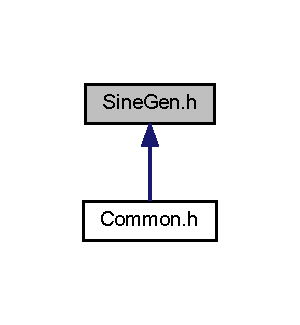
\includegraphics[width=144pt]{_sine_gen_8h__dep__incl}
\end{center}
\end{figure}
\subsection*{Macros}
\begin{DoxyCompactItemize}
\item 
\#define \hyperlink{_sine_gen_8h_afc105af9d8f851266d0b8e8ffe57931a}{S\-I\-N\-\_\-\-D\-F\-L\-T\-\_\-\-R\-C\-T\-F\-Y}~T\-R\-U\-E
\item 
\#define \hyperlink{_sine_gen_8h_a9c042423a04dc371b1c79ecc1f16e813}{S\-I\-N\-\_\-\-D\-F\-L\-T\-\_\-\-O\-F\-S\-T}~0
\item 
\#define \hyperlink{_sine_gen_8h_ae88ab3e38bc960b4c0e15f9712d25f72}{S\-I\-N\-\_\-\-D\-F\-L\-T\-\_\-\-P\-H\-S\-E}~0
\item 
\#define \hyperlink{_sine_gen_8h_aa63a6918009b4e4381e359cee2f05eef}{S\-I\-N\-\_\-\-D\-F\-L\-T\-\_\-\-G\-A\-I\-N}~0.\-9
\item 
\#define \hyperlink{_sine_gen_8h_aa1d98c477c6de604fc6ca986f2d83238}{S\-I\-N\-\_\-\-D\-F\-L\-T\-\_\-\-F}~50.\-0
\item 
\#define \hyperlink{_sine_gen_8h_a1640e33dcd5a970b4a9731ec68125bd6}{S\-I\-N\-\_\-\-D\-F\-L\-T\-\_\-\-F\-\_\-\-M\-A\-X}~1000u
\item 
\#define \hyperlink{_sine_gen_8h_a71b6211a4d077af219d7e503f17114d1}{S\-I\-N\-\_\-\-C\-H\-A\-N\-N\-E\-L}~\hyperlink{_macro_nets_8h_a3fc4318ae73eae35339f616047300b0f}{A\-C\-\_\-\-S\-T\-A\-G\-E}
\item 
\#define \hyperlink{_sine_gen_8h_a8d1689d7437a3410059f1f377ec63ebd}{S\-I\-N\-\_\-\-F\-\_\-\-S\-P\-L}~8250u
\end{DoxyCompactItemize}
\subsection*{Functions}
\begin{DoxyCompactItemize}
\item 
void \hyperlink{_sine_gen_8h_a41e810f7181a4ecaa5bc5f0713c6db89}{sg\-Init} (void)
\item 
void \hyperlink{_sine_gen_8h_a4ad7c6eca0c2bcdadaa81dd3fbb9df4b}{sg\-Update} (void)
\item 
void \hyperlink{_sine_gen_8h_a9d1f773315008eac3fc68486f3c9b02a}{sg\-Gain\-Update} (void)
\item 
Uint16 \hyperlink{_sine_gen_8h_a4da3578fed6e04e782a037a270ebde65}{sg\-Set\-State} (Uint16 stt)
\item 
Uint16 \hyperlink{_sine_gen_8h_a663b333309e306b76cc538d8b057ca7d}{sg\-Set\-Rectify} (Uint16 rfy)
\item 
Uint16 \hyperlink{_sine_gen_8h_ac4fa27b2a1e42815c53a9c41aea39dae}{sg\-Set\-Offset} (float32 ofst)
\item 
Uint16 \hyperlink{_sine_gen_8h_ac0b4e573457d4a6e3102c17ec9c3281a}{sg\-Set\-Initial\-Phase} (float32 phs)
\item 
Uint16 \hyperlink{_sine_gen_8h_a1352efb3adb6289a295afa3961d4a352}{sg\-Set\-Gain\-Target} (float32 gnt)
\item 
Uint16 \hyperlink{_sine_gen_8h_a3be6fb433900f4d91074b337ea3dba58}{sg\-Set\-Freq} (Uint16 frq)
\item 
Uint16 \hyperlink{_sine_gen_8h_a42044b7a7555c9bf2a1927f11762a340}{sg\-Set\-F\-Max} (Uint16 frq)
\item 
Uint16 \hyperlink{_sine_gen_8h_a65e0faae0e2f43f55395dc7b310d3702}{sg\-Set\-Step\-Max} (Uint16 s\-Mx)
\item 
Uint16 \hyperlink{_sine_gen_8h_ab720e3168a284abe388edf230705e4b4}{sg\-Get\-State} (Uint16 $\ast$stt\-Dest)
\item 
Uint16 \hyperlink{_sine_gen_8h_a2257f55d8be03a940f80091c77b70b59}{sg\-Get\-Rectify} (Uint16 $\ast$rfy\-Dest)
\item 
Uint16 \hyperlink{_sine_gen_8h_a56832d4be61bfbb6263eef6100515365}{sg\-Get\-Offset} (float32 $\ast$oft\-Dest)
\item 
Uint16 \hyperlink{_sine_gen_8h_aaf39e7e31c43b94af71863a1ca3c5704}{sg\-Get\-Gain\-Target} (float32 $\ast$gnt\-Dest)
\item 
Uint16 \hyperlink{_sine_gen_8h_a927bad9dd75bf9372d0becfe714a66c7}{sg\-Get\-Freq} (Uint16 $\ast$frq\-Dest)
\item 
Uint16 \hyperlink{_sine_gen_8h_a455fbafea83fb0add030a099ed30613f}{sg\-Get\-F\-Max} (Uint16 $\ast$frq\-Dest)
\item 
Uint16 \hyperlink{_sine_gen_8h_a3b21cabaadf0129ad90fdc9a8d6f4746}{sg\-Get\-Step\-Max} (Uint16 $\ast$s\-Mx\-Dest)
\item 
Uint16 \hyperlink{_sine_gen_8h_ad625f20b4e4f394215e615071b9217b0}{sg\-Get\-Resolution} (float32 $\ast$rsl\-Dest)
\end{DoxyCompactItemize}
\subsection*{Variables}
\begin{DoxyCompactItemize}
\item 
volatile int32 $\ast$ \hyperlink{_sine_gen_8h_a5dba1fe543c9e62ef6cc8cf4179de951}{S\-G\-E\-N\-T\-I\-\_\-1ch\-\_\-\-V\-Out}
\item 
volatile int32 $\ast$ \hyperlink{_sine_gen_8h_a5369a96cf47ea2fbd84a92ed4091b48b}{S\-G\-E\-N\-T\-I\-\_\-1ch\-\_\-\-Sign}
\end{DoxyCompactItemize}


\subsection{Detailed Description}
Signal generator functions. \hyperlink{_sine_gen_8h_a41e810f7181a4ecaa5bc5f0713c6db89}{sg\-Init()} must be called before any other signal generator functions are used. Note that the frequency resolution is determined by the maximum frequency and the step max. For further details, see the signal generator library documentation (Texas Instruments Signal Generator Library Module user's Guide).

\begin{DoxyWarning}{Warning}
This file is included by the file I\-S\-R.\-asm. 
\end{DoxyWarning}


\subsection{Macro Definition Documentation}
\hypertarget{_sine_gen_8h_a71b6211a4d077af219d7e503f17114d1}{\index{Sine\-Gen.\-h@{Sine\-Gen.\-h}!S\-I\-N\-\_\-\-C\-H\-A\-N\-N\-E\-L@{S\-I\-N\-\_\-\-C\-H\-A\-N\-N\-E\-L}}
\index{S\-I\-N\-\_\-\-C\-H\-A\-N\-N\-E\-L@{S\-I\-N\-\_\-\-C\-H\-A\-N\-N\-E\-L}!SineGen.h@{Sine\-Gen.\-h}}
\subsubsection[{S\-I\-N\-\_\-\-C\-H\-A\-N\-N\-E\-L}]{\setlength{\rightskip}{0pt plus 5cm}\#define S\-I\-N\-\_\-\-C\-H\-A\-N\-N\-E\-L~{\bf A\-C\-\_\-\-S\-T\-A\-G\-E}}}\label{_sine_gen_8h_a71b6211a4d077af219d7e503f17114d1}
Defines which channel enable controls the generator output. \hypertarget{_sine_gen_8h_aa1d98c477c6de604fc6ca986f2d83238}{\index{Sine\-Gen.\-h@{Sine\-Gen.\-h}!S\-I\-N\-\_\-\-D\-F\-L\-T\-\_\-\-F@{S\-I\-N\-\_\-\-D\-F\-L\-T\-\_\-\-F}}
\index{S\-I\-N\-\_\-\-D\-F\-L\-T\-\_\-\-F@{S\-I\-N\-\_\-\-D\-F\-L\-T\-\_\-\-F}!SineGen.h@{Sine\-Gen.\-h}}
\subsubsection[{S\-I\-N\-\_\-\-D\-F\-L\-T\-\_\-\-F}]{\setlength{\rightskip}{0pt plus 5cm}\#define S\-I\-N\-\_\-\-D\-F\-L\-T\-\_\-\-F~50.\-0}}\label{_sine_gen_8h_aa1d98c477c6de604fc6ca986f2d83238}
Initial frequency setting (hertz). \hypertarget{_sine_gen_8h_a1640e33dcd5a970b4a9731ec68125bd6}{\index{Sine\-Gen.\-h@{Sine\-Gen.\-h}!S\-I\-N\-\_\-\-D\-F\-L\-T\-\_\-\-F\-\_\-\-M\-A\-X@{S\-I\-N\-\_\-\-D\-F\-L\-T\-\_\-\-F\-\_\-\-M\-A\-X}}
\index{S\-I\-N\-\_\-\-D\-F\-L\-T\-\_\-\-F\-\_\-\-M\-A\-X@{S\-I\-N\-\_\-\-D\-F\-L\-T\-\_\-\-F\-\_\-\-M\-A\-X}!SineGen.h@{Sine\-Gen.\-h}}
\subsubsection[{S\-I\-N\-\_\-\-D\-F\-L\-T\-\_\-\-F\-\_\-\-M\-A\-X}]{\setlength{\rightskip}{0pt plus 5cm}\#define S\-I\-N\-\_\-\-D\-F\-L\-T\-\_\-\-F\-\_\-\-M\-A\-X~1000u}}\label{_sine_gen_8h_a1640e33dcd5a970b4a9731ec68125bd6}
Initial maximum frequency setting (hertz). \hypertarget{_sine_gen_8h_aa63a6918009b4e4381e359cee2f05eef}{\index{Sine\-Gen.\-h@{Sine\-Gen.\-h}!S\-I\-N\-\_\-\-D\-F\-L\-T\-\_\-\-G\-A\-I\-N@{S\-I\-N\-\_\-\-D\-F\-L\-T\-\_\-\-G\-A\-I\-N}}
\index{S\-I\-N\-\_\-\-D\-F\-L\-T\-\_\-\-G\-A\-I\-N@{S\-I\-N\-\_\-\-D\-F\-L\-T\-\_\-\-G\-A\-I\-N}!SineGen.h@{Sine\-Gen.\-h}}
\subsubsection[{S\-I\-N\-\_\-\-D\-F\-L\-T\-\_\-\-G\-A\-I\-N}]{\setlength{\rightskip}{0pt plus 5cm}\#define S\-I\-N\-\_\-\-D\-F\-L\-T\-\_\-\-G\-A\-I\-N~0.\-9}}\label{_sine_gen_8h_aa63a6918009b4e4381e359cee2f05eef}
Initial gain setting \mbox{[}0.\-0, 1.\-0\mbox{]}. \hypertarget{_sine_gen_8h_a9c042423a04dc371b1c79ecc1f16e813}{\index{Sine\-Gen.\-h@{Sine\-Gen.\-h}!S\-I\-N\-\_\-\-D\-F\-L\-T\-\_\-\-O\-F\-S\-T@{S\-I\-N\-\_\-\-D\-F\-L\-T\-\_\-\-O\-F\-S\-T}}
\index{S\-I\-N\-\_\-\-D\-F\-L\-T\-\_\-\-O\-F\-S\-T@{S\-I\-N\-\_\-\-D\-F\-L\-T\-\_\-\-O\-F\-S\-T}!SineGen.h@{Sine\-Gen.\-h}}
\subsubsection[{S\-I\-N\-\_\-\-D\-F\-L\-T\-\_\-\-O\-F\-S\-T}]{\setlength{\rightskip}{0pt plus 5cm}\#define S\-I\-N\-\_\-\-D\-F\-L\-T\-\_\-\-O\-F\-S\-T~0}}\label{_sine_gen_8h_a9c042423a04dc371b1c79ecc1f16e813}
Initial offset setting \mbox{[}-\/0.\-5, +0.5\mbox{]}, I\-Q15. \hypertarget{_sine_gen_8h_ae88ab3e38bc960b4c0e15f9712d25f72}{\index{Sine\-Gen.\-h@{Sine\-Gen.\-h}!S\-I\-N\-\_\-\-D\-F\-L\-T\-\_\-\-P\-H\-S\-E@{S\-I\-N\-\_\-\-D\-F\-L\-T\-\_\-\-P\-H\-S\-E}}
\index{S\-I\-N\-\_\-\-D\-F\-L\-T\-\_\-\-P\-H\-S\-E@{S\-I\-N\-\_\-\-D\-F\-L\-T\-\_\-\-P\-H\-S\-E}!SineGen.h@{Sine\-Gen.\-h}}
\subsubsection[{S\-I\-N\-\_\-\-D\-F\-L\-T\-\_\-\-P\-H\-S\-E}]{\setlength{\rightskip}{0pt plus 5cm}\#define S\-I\-N\-\_\-\-D\-F\-L\-T\-\_\-\-P\-H\-S\-E~0}}\label{_sine_gen_8h_ae88ab3e38bc960b4c0e15f9712d25f72}
Initial initial phase setting \mbox{[}0, 360), I\-Q16. \hypertarget{_sine_gen_8h_afc105af9d8f851266d0b8e8ffe57931a}{\index{Sine\-Gen.\-h@{Sine\-Gen.\-h}!S\-I\-N\-\_\-\-D\-F\-L\-T\-\_\-\-R\-C\-T\-F\-Y@{S\-I\-N\-\_\-\-D\-F\-L\-T\-\_\-\-R\-C\-T\-F\-Y}}
\index{S\-I\-N\-\_\-\-D\-F\-L\-T\-\_\-\-R\-C\-T\-F\-Y@{S\-I\-N\-\_\-\-D\-F\-L\-T\-\_\-\-R\-C\-T\-F\-Y}!SineGen.h@{Sine\-Gen.\-h}}
\subsubsection[{S\-I\-N\-\_\-\-D\-F\-L\-T\-\_\-\-R\-C\-T\-F\-Y}]{\setlength{\rightskip}{0pt plus 5cm}\#define S\-I\-N\-\_\-\-D\-F\-L\-T\-\_\-\-R\-C\-T\-F\-Y~T\-R\-U\-E}}\label{_sine_gen_8h_afc105af9d8f851266d0b8e8ffe57931a}
Initial rectification setting \mbox{[}T\-R\-U\-E $|$ F\-A\-L\-S\-E). \hypertarget{_sine_gen_8h_a8d1689d7437a3410059f1f377ec63ebd}{\index{Sine\-Gen.\-h@{Sine\-Gen.\-h}!S\-I\-N\-\_\-\-F\-\_\-\-S\-P\-L@{S\-I\-N\-\_\-\-F\-\_\-\-S\-P\-L}}
\index{S\-I\-N\-\_\-\-F\-\_\-\-S\-P\-L@{S\-I\-N\-\_\-\-F\-\_\-\-S\-P\-L}!SineGen.h@{Sine\-Gen.\-h}}
\subsubsection[{S\-I\-N\-\_\-\-F\-\_\-\-S\-P\-L}]{\setlength{\rightskip}{0pt plus 5cm}\#define S\-I\-N\-\_\-\-F\-\_\-\-S\-P\-L~8250u}}\label{_sine_gen_8h_a8d1689d7437a3410059f1f377ec63ebd}
Signal sampling frequency, i.\-e. the frequency that sgen.\-calc() is called at. This is dependent on I\-S\-R frequency, currently 1/4 of f\-\_\-\-I\-S\-R, full I\-S\-R speed is 33,000\-Hz. 

\subsection{Function Documentation}
\hypertarget{_sine_gen_8h_a9d1f773315008eac3fc68486f3c9b02a}{\index{Sine\-Gen.\-h@{Sine\-Gen.\-h}!sg\-Gain\-Update@{sg\-Gain\-Update}}
\index{sg\-Gain\-Update@{sg\-Gain\-Update}!SineGen.h@{Sine\-Gen.\-h}}
\subsubsection[{sg\-Gain\-Update}]{\setlength{\rightskip}{0pt plus 5cm}void sg\-Gain\-Update (
\begin{DoxyParamCaption}
\item[{void}]{}
\end{DoxyParamCaption}
)}}\label{_sine_gen_8h_a9d1f773315008eac3fc68486f3c9b02a}
Updates the gain value to create a slow-\/start ramp. This should be called at the same time and similarly to the D\-C slew update. \begin{DoxySeeAlso}{See Also}
\hyperlink{_slew_control_8h_a8f8f2b1ef59b7fa90122e5609e24cd06}{sc\-Slew\-Update()} 
\end{DoxySeeAlso}
\hypertarget{_sine_gen_8h_a455fbafea83fb0add030a099ed30613f}{\index{Sine\-Gen.\-h@{Sine\-Gen.\-h}!sg\-Get\-F\-Max@{sg\-Get\-F\-Max}}
\index{sg\-Get\-F\-Max@{sg\-Get\-F\-Max}!SineGen.h@{Sine\-Gen.\-h}}
\subsubsection[{sg\-Get\-F\-Max}]{\setlength{\rightskip}{0pt plus 5cm}Uint16 sg\-Get\-F\-Max (
\begin{DoxyParamCaption}
\item[{Uint16 $\ast$}]{frq\-Dest}
\end{DoxyParamCaption}
)}}\label{_sine_gen_8h_a455fbafea83fb0add030a099ed30613f}
Queries the current maximum frequecny setting. 
\begin{DoxyParams}[1]{Parameters}
\mbox{\tt out}  & {\em frq\-Dest} & Address of the memory location at which to place the query result (hertz). \\
\hline
\end{DoxyParams}
\begin{DoxyReturn}{Returns}
Error ststus. 
\end{DoxyReturn}
\hypertarget{_sine_gen_8h_a927bad9dd75bf9372d0becfe714a66c7}{\index{Sine\-Gen.\-h@{Sine\-Gen.\-h}!sg\-Get\-Freq@{sg\-Get\-Freq}}
\index{sg\-Get\-Freq@{sg\-Get\-Freq}!SineGen.h@{Sine\-Gen.\-h}}
\subsubsection[{sg\-Get\-Freq}]{\setlength{\rightskip}{0pt plus 5cm}Uint16 sg\-Get\-Freq (
\begin{DoxyParamCaption}
\item[{Uint16 $\ast$}]{frq\-Dest}
\end{DoxyParamCaption}
)}}\label{_sine_gen_8h_a927bad9dd75bf9372d0becfe714a66c7}
Queries the current frequency setting. 
\begin{DoxyParams}[1]{Parameters}
\mbox{\tt out}  & {\em frq\-Dest} & Address of the memory location at which to place the query result (hertz). \\
\hline
\end{DoxyParams}
\begin{DoxyReturn}{Returns}
Error status. 
\end{DoxyReturn}
\hypertarget{_sine_gen_8h_aaf39e7e31c43b94af71863a1ca3c5704}{\index{Sine\-Gen.\-h@{Sine\-Gen.\-h}!sg\-Get\-Gain\-Target@{sg\-Get\-Gain\-Target}}
\index{sg\-Get\-Gain\-Target@{sg\-Get\-Gain\-Target}!SineGen.h@{Sine\-Gen.\-h}}
\subsubsection[{sg\-Get\-Gain\-Target}]{\setlength{\rightskip}{0pt plus 5cm}Uint16 sg\-Get\-Gain\-Target (
\begin{DoxyParamCaption}
\item[{float32 $\ast$}]{gnt\-Dest}
\end{DoxyParamCaption}
)}}\label{_sine_gen_8h_aaf39e7e31c43b94af71863a1ca3c5704}
Queries the current target gain setting. 
\begin{DoxyParams}[1]{Parameters}
\mbox{\tt out}  & {\em gnt\-Dest} & Address of the memory location at which to place the query result. \\
\hline
\end{DoxyParams}
\begin{DoxyReturn}{Returns}
Error status. 
\end{DoxyReturn}
\hypertarget{_sine_gen_8h_a56832d4be61bfbb6263eef6100515365}{\index{Sine\-Gen.\-h@{Sine\-Gen.\-h}!sg\-Get\-Offset@{sg\-Get\-Offset}}
\index{sg\-Get\-Offset@{sg\-Get\-Offset}!SineGen.h@{Sine\-Gen.\-h}}
\subsubsection[{sg\-Get\-Offset}]{\setlength{\rightskip}{0pt plus 5cm}Uint16 sg\-Get\-Offset (
\begin{DoxyParamCaption}
\item[{float32 $\ast$}]{oft\-Dest}
\end{DoxyParamCaption}
)}}\label{_sine_gen_8h_a56832d4be61bfbb6263eef6100515365}
Queries the current signal D\-C offset setting. 
\begin{DoxyParams}[1]{Parameters}
\mbox{\tt out}  & {\em oft\-Dest} & Address of the memory location at which to place the query result. \\
\hline
\end{DoxyParams}
\begin{DoxyReturn}{Returns}
Error status. 
\end{DoxyReturn}
\hypertarget{_sine_gen_8h_a2257f55d8be03a940f80091c77b70b59}{\index{Sine\-Gen.\-h@{Sine\-Gen.\-h}!sg\-Get\-Rectify@{sg\-Get\-Rectify}}
\index{sg\-Get\-Rectify@{sg\-Get\-Rectify}!SineGen.h@{Sine\-Gen.\-h}}
\subsubsection[{sg\-Get\-Rectify}]{\setlength{\rightskip}{0pt plus 5cm}Uint16 sg\-Get\-Rectify (
\begin{DoxyParamCaption}
\item[{Uint16 $\ast$}]{rfy\-Dest}
\end{DoxyParamCaption}
)}}\label{_sine_gen_8h_a2257f55d8be03a940f80091c77b70b59}
Queries the current state of the signal generator rectification enable. 
\begin{DoxyParams}[1]{Parameters}
\mbox{\tt out}  & {\em rfy\-Dest} & Address of the memory location at which to place the query result (1\-:O\-N $|$ 0\-:O\-F\-F). \\
\hline
\end{DoxyParams}
\begin{DoxyReturn}{Returns}
Error status. 
\end{DoxyReturn}
\hypertarget{_sine_gen_8h_ad625f20b4e4f394215e615071b9217b0}{\index{Sine\-Gen.\-h@{Sine\-Gen.\-h}!sg\-Get\-Resolution@{sg\-Get\-Resolution}}
\index{sg\-Get\-Resolution@{sg\-Get\-Resolution}!SineGen.h@{Sine\-Gen.\-h}}
\subsubsection[{sg\-Get\-Resolution}]{\setlength{\rightskip}{0pt plus 5cm}Uint16 sg\-Get\-Resolution (
\begin{DoxyParamCaption}
\item[{float32 $\ast$}]{rsl\-Dest}
\end{DoxyParamCaption}
)}}\label{_sine_gen_8h_ad625f20b4e4f394215e615071b9217b0}
Queries the current frequency resolution. This is equal to $ f_{max}$ / step\-\_\-max. 
\begin{DoxyParams}[1]{Parameters}
\mbox{\tt out}  & {\em rsl\-Dest} & Address of the memory location at which to place the query result. \\
\hline
\end{DoxyParams}
\begin{DoxyReturn}{Returns}
Error status. 
\end{DoxyReturn}
\hypertarget{_sine_gen_8h_ab720e3168a284abe388edf230705e4b4}{\index{Sine\-Gen.\-h@{Sine\-Gen.\-h}!sg\-Get\-State@{sg\-Get\-State}}
\index{sg\-Get\-State@{sg\-Get\-State}!SineGen.h@{Sine\-Gen.\-h}}
\subsubsection[{sg\-Get\-State}]{\setlength{\rightskip}{0pt plus 5cm}Uint16 sg\-Get\-State (
\begin{DoxyParamCaption}
\item[{Uint16 $\ast$}]{stt\-Dest}
\end{DoxyParamCaption}
)}}\label{_sine_gen_8h_ab720e3168a284abe388edf230705e4b4}
Queries the current state of the generator output. 
\begin{DoxyParams}[1]{Parameters}
\mbox{\tt out}  & {\em stt\-Dest} & Address of the memory location at which to place the query result (1\-:O\-N $|$ 0\-:O\-F\-F). \\
\hline
\end{DoxyParams}
\begin{DoxyReturn}{Returns}
Error status. 
\end{DoxyReturn}
\hypertarget{_sine_gen_8h_a3b21cabaadf0129ad90fdc9a8d6f4746}{\index{Sine\-Gen.\-h@{Sine\-Gen.\-h}!sg\-Get\-Step\-Max@{sg\-Get\-Step\-Max}}
\index{sg\-Get\-Step\-Max@{sg\-Get\-Step\-Max}!SineGen.h@{Sine\-Gen.\-h}}
\subsubsection[{sg\-Get\-Step\-Max}]{\setlength{\rightskip}{0pt plus 5cm}Uint16 sg\-Get\-Step\-Max (
\begin{DoxyParamCaption}
\item[{Uint16 $\ast$}]{s\-Mx\-Dest}
\end{DoxyParamCaption}
)}}\label{_sine_gen_8h_a3b21cabaadf0129ad90fdc9a8d6f4746}
Queries the current step\-\_\-max setting. 
\begin{DoxyParams}[1]{Parameters}
\mbox{\tt out}  & {\em s\-Mx\-Dest} & Address of the memory location at which to place the query result. \\
\hline
\end{DoxyParams}
\begin{DoxyReturn}{Returns}
Error status. 
\end{DoxyReturn}
\hypertarget{_sine_gen_8h_a41e810f7181a4ecaa5bc5f0713c6db89}{\index{Sine\-Gen.\-h@{Sine\-Gen.\-h}!sg\-Init@{sg\-Init}}
\index{sg\-Init@{sg\-Init}!SineGen.h@{Sine\-Gen.\-h}}
\subsubsection[{sg\-Init}]{\setlength{\rightskip}{0pt plus 5cm}void sg\-Init (
\begin{DoxyParamCaption}
\item[{void}]{}
\end{DoxyParamCaption}
)}}\label{_sine_gen_8h_a41e810f7181a4ecaa5bc5f0713c6db89}
Sets the initial generator values and disables the output. This function M\-U\-S\-T be called before any other signal generator function. \hypertarget{_sine_gen_8h_a42044b7a7555c9bf2a1927f11762a340}{\index{Sine\-Gen.\-h@{Sine\-Gen.\-h}!sg\-Set\-F\-Max@{sg\-Set\-F\-Max}}
\index{sg\-Set\-F\-Max@{sg\-Set\-F\-Max}!SineGen.h@{Sine\-Gen.\-h}}
\subsubsection[{sg\-Set\-F\-Max}]{\setlength{\rightskip}{0pt plus 5cm}Uint16 sg\-Set\-F\-Max (
\begin{DoxyParamCaption}
\item[{Uint16}]{frq}
\end{DoxyParamCaption}
)}}\label{_sine_gen_8h_a42044b7a7555c9bf2a1927f11762a340}
Sets the signal generator maximum frequency setting value, $ f_{max}$ . 
\begin{DoxyParams}[1]{Parameters}
\mbox{\tt in}  & {\em frq} & Frequency value \mbox{[}0, $ f_{sample}$) (hertz). \\
\hline
\end{DoxyParams}
\begin{DoxyReturn}{Returns}
Error status. 
\end{DoxyReturn}
\hypertarget{_sine_gen_8h_a3be6fb433900f4d91074b337ea3dba58}{\index{Sine\-Gen.\-h@{Sine\-Gen.\-h}!sg\-Set\-Freq@{sg\-Set\-Freq}}
\index{sg\-Set\-Freq@{sg\-Set\-Freq}!SineGen.h@{Sine\-Gen.\-h}}
\subsubsection[{sg\-Set\-Freq}]{\setlength{\rightskip}{0pt plus 5cm}Uint16 sg\-Set\-Freq (
\begin{DoxyParamCaption}
\item[{Uint16}]{frq}
\end{DoxyParamCaption}
)}}\label{_sine_gen_8h_a3be6fb433900f4d91074b337ea3dba58}
Sets the signal frequency. 
\begin{DoxyParams}[1]{Parameters}
\mbox{\tt in}  & {\em frq} & Frequency value \mbox{[}0, $ f_{max}$) (hertz). \\
\hline
\end{DoxyParams}
\begin{DoxyReturn}{Returns}
Error status. 
\end{DoxyReturn}
\hypertarget{_sine_gen_8h_a1352efb3adb6289a295afa3961d4a352}{\index{Sine\-Gen.\-h@{Sine\-Gen.\-h}!sg\-Set\-Gain\-Target@{sg\-Set\-Gain\-Target}}
\index{sg\-Set\-Gain\-Target@{sg\-Set\-Gain\-Target}!SineGen.h@{Sine\-Gen.\-h}}
\subsubsection[{sg\-Set\-Gain\-Target}]{\setlength{\rightskip}{0pt plus 5cm}Uint16 sg\-Set\-Gain\-Target (
\begin{DoxyParamCaption}
\item[{float32}]{gnt}
\end{DoxyParamCaption}
)}}\label{_sine_gen_8h_a1352efb3adb6289a295afa3961d4a352}
Sets the target gain of the signal. 
\begin{DoxyParams}[1]{Parameters}
\mbox{\tt in}  & {\em gnt} & Gain target value \mbox{[}0.\-0, 1.\-0). \\
\hline
\end{DoxyParams}
\begin{DoxyReturn}{Returns}
Error status. 
\end{DoxyReturn}
\hypertarget{_sine_gen_8h_ac0b4e573457d4a6e3102c17ec9c3281a}{\index{Sine\-Gen.\-h@{Sine\-Gen.\-h}!sg\-Set\-Initial\-Phase@{sg\-Set\-Initial\-Phase}}
\index{sg\-Set\-Initial\-Phase@{sg\-Set\-Initial\-Phase}!SineGen.h@{Sine\-Gen.\-h}}
\subsubsection[{sg\-Set\-Initial\-Phase}]{\setlength{\rightskip}{0pt plus 5cm}Uint16 sg\-Set\-Initial\-Phase (
\begin{DoxyParamCaption}
\item[{float32}]{phs}
\end{DoxyParamCaption}
)}}\label{_sine_gen_8h_ac0b4e573457d4a6e3102c17ec9c3281a}
Sets the signal initial phase value 
\begin{DoxyParams}[1]{Parameters}
\mbox{\tt in}  & {\em phs} & Initial phase value \mbox{[}0, 360) (degrees). \\
\hline
\end{DoxyParams}
\begin{DoxyReturn}{Returns}
Error status 
\end{DoxyReturn}
\hypertarget{_sine_gen_8h_ac4fa27b2a1e42815c53a9c41aea39dae}{\index{Sine\-Gen.\-h@{Sine\-Gen.\-h}!sg\-Set\-Offset@{sg\-Set\-Offset}}
\index{sg\-Set\-Offset@{sg\-Set\-Offset}!SineGen.h@{Sine\-Gen.\-h}}
\subsubsection[{sg\-Set\-Offset}]{\setlength{\rightskip}{0pt plus 5cm}Uint16 sg\-Set\-Offset (
\begin{DoxyParamCaption}
\item[{float32}]{ofst}
\end{DoxyParamCaption}
)}}\label{_sine_gen_8h_ac4fa27b2a1e42815c53a9c41aea39dae}
Sets the signal D\-C offset 
\begin{DoxyParams}[1]{Parameters}
\mbox{\tt in}  & {\em ofst} & D\-C offset value \mbox{[}-\/0.\-5, +0.5). \\
\hline
\end{DoxyParams}
\begin{DoxyReturn}{Returns}
Error status. 
\end{DoxyReturn}
\hypertarget{_sine_gen_8h_a663b333309e306b76cc538d8b057ca7d}{\index{Sine\-Gen.\-h@{Sine\-Gen.\-h}!sg\-Set\-Rectify@{sg\-Set\-Rectify}}
\index{sg\-Set\-Rectify@{sg\-Set\-Rectify}!SineGen.h@{Sine\-Gen.\-h}}
\subsubsection[{sg\-Set\-Rectify}]{\setlength{\rightskip}{0pt plus 5cm}Uint16 sg\-Set\-Rectify (
\begin{DoxyParamCaption}
\item[{Uint16}]{rfy}
\end{DoxyParamCaption}
)}}\label{_sine_gen_8h_a663b333309e306b76cc538d8b057ca7d}
Enables or disables the rectification of the generator output 
\begin{DoxyParams}[1]{Parameters}
\mbox{\tt in}  & {\em rfy} & Rectification enable state (1\-:O\-N $|$ 0\-:O\-F\-F). \\
\hline
\end{DoxyParams}
\begin{DoxyReturn}{Returns}
Error status. 
\end{DoxyReturn}
\hypertarget{_sine_gen_8h_a4da3578fed6e04e782a037a270ebde65}{\index{Sine\-Gen.\-h@{Sine\-Gen.\-h}!sg\-Set\-State@{sg\-Set\-State}}
\index{sg\-Set\-State@{sg\-Set\-State}!SineGen.h@{Sine\-Gen.\-h}}
\subsubsection[{sg\-Set\-State}]{\setlength{\rightskip}{0pt plus 5cm}Uint16 sg\-Set\-State (
\begin{DoxyParamCaption}
\item[{Uint16}]{stt}
\end{DoxyParamCaption}
)}}\label{_sine_gen_8h_a4da3578fed6e04e782a037a270ebde65}
Enables or disables the output of the generator onto the connected net 
\begin{DoxyParams}[1]{Parameters}
\mbox{\tt in}  & {\em stt} & Output enable state (1\-:O\-N $|$ 0\-:O\-F\-F). \\
\hline
\end{DoxyParams}
\begin{DoxyReturn}{Returns}
Error status. 
\end{DoxyReturn}
\hypertarget{_sine_gen_8h_a65e0faae0e2f43f55395dc7b310d3702}{\index{Sine\-Gen.\-h@{Sine\-Gen.\-h}!sg\-Set\-Step\-Max@{sg\-Set\-Step\-Max}}
\index{sg\-Set\-Step\-Max@{sg\-Set\-Step\-Max}!SineGen.h@{Sine\-Gen.\-h}}
\subsubsection[{sg\-Set\-Step\-Max}]{\setlength{\rightskip}{0pt plus 5cm}Uint16 sg\-Set\-Step\-Max (
\begin{DoxyParamCaption}
\item[{Uint16}]{s\-Mx}
\end{DoxyParamCaption}
)}}\label{_sine_gen_8h_a65e0faae0e2f43f55395dc7b310d3702}
Sets the signal generator step max setting value. 
\begin{DoxyParams}[1]{Parameters}
\mbox{\tt in}  & {\em s\-Mx} & Step\-\_\-max value \mbox{[}0, 32767). \\
\hline
\end{DoxyParams}
\begin{DoxyReturn}{Returns}
Error status. 
\end{DoxyReturn}
\hypertarget{_sine_gen_8h_a4ad7c6eca0c2bcdadaa81dd3fbb9df4b}{\index{Sine\-Gen.\-h@{Sine\-Gen.\-h}!sg\-Update@{sg\-Update}}
\index{sg\-Update@{sg\-Update}!SineGen.h@{Sine\-Gen.\-h}}
\subsubsection[{sg\-Update}]{\setlength{\rightskip}{0pt plus 5cm}void sg\-Update (
\begin{DoxyParamCaption}
\item[{void}]{}
\end{DoxyParamCaption}
)}}\label{_sine_gen_8h_a4ad7c6eca0c2bcdadaa81dd3fbb9df4b}
Generates the next signal data point and loads it onto the V\-Out terminal. If the point is positive the sign terminal is set, otherwise it is cleared. If rectify is enabled, the value produced will be an absolute value. 

\subsection{Variable Documentation}
\hypertarget{_sine_gen_8h_a5369a96cf47ea2fbd84a92ed4091b48b}{\index{Sine\-Gen.\-h@{Sine\-Gen.\-h}!S\-G\-E\-N\-T\-I\-\_\-1ch\-\_\-\-Sign@{S\-G\-E\-N\-T\-I\-\_\-1ch\-\_\-\-Sign}}
\index{S\-G\-E\-N\-T\-I\-\_\-1ch\-\_\-\-Sign@{S\-G\-E\-N\-T\-I\-\_\-1ch\-\_\-\-Sign}!SineGen.h@{Sine\-Gen.\-h}}
\subsubsection[{S\-G\-E\-N\-T\-I\-\_\-1ch\-\_\-\-Sign}]{\setlength{\rightskip}{0pt plus 5cm}volatile int32$\ast$ S\-G\-E\-N\-T\-I\-\_\-1ch\-\_\-\-Sign}}\label{_sine_gen_8h_a5369a96cf47ea2fbd84a92ed4091b48b}
Voltage sign (pre-\/rectification) output terminal. \hypertarget{_sine_gen_8h_a5dba1fe543c9e62ef6cc8cf4179de951}{\index{Sine\-Gen.\-h@{Sine\-Gen.\-h}!S\-G\-E\-N\-T\-I\-\_\-1ch\-\_\-\-V\-Out@{S\-G\-E\-N\-T\-I\-\_\-1ch\-\_\-\-V\-Out}}
\index{S\-G\-E\-N\-T\-I\-\_\-1ch\-\_\-\-V\-Out@{S\-G\-E\-N\-T\-I\-\_\-1ch\-\_\-\-V\-Out}!SineGen.h@{Sine\-Gen.\-h}}
\subsubsection[{S\-G\-E\-N\-T\-I\-\_\-1ch\-\_\-\-V\-Out}]{\setlength{\rightskip}{0pt plus 5cm}volatile int32$\ast$ S\-G\-E\-N\-T\-I\-\_\-1ch\-\_\-\-V\-Out}}\label{_sine_gen_8h_a5dba1fe543c9e62ef6cc8cf4179de951}
Voltage output terminal. 
\hypertarget{_slew_control_8h}{\section{Slew\-Control.\-h File Reference}
\label{_slew_control_8h}\index{Slew\-Control.\-h@{Slew\-Control.\-h}}
}


Slew control functions.  


This graph shows which files directly or indirectly include this file\-:\nopagebreak
\begin{figure}[H]
\begin{center}
\leavevmode
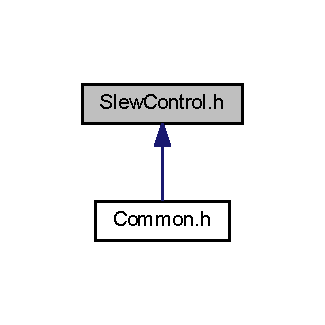
\includegraphics[width=156pt]{_slew_control_8h__dep__incl}
\end{center}
\end{figure}
\subsection*{Functions}
\begin{DoxyCompactItemize}
\item 
void \hyperlink{_slew_control_8h_a8f8f2b1ef59b7fa90122e5609e24cd06}{sc\-Slew\-Update} (void)
\item 
Uint16 \hyperlink{_slew_control_8h_acd4f1d77c353f333438ae688a9bcc8fe}{sc\-Set\-Target} (Uint16 chnl, float32 trgt)
\item 
Uint16 \hyperlink{_slew_control_8h_a91e197a77f8f6c05dc478431164114a4}{sc\-Set\-Step} (Uint16 chnl, float32 stp)
\item 
Uint16 \hyperlink{_slew_control_8h_a92578a062af02eb967ca2dfbd68b00cf}{sc\-Set\-State} (Uint16 chnl, Uint16 stt)
\item 
Uint16 \hyperlink{_slew_control_8h_a1e7d07e1a6d9b1e40b1b39d97df638b9}{sc\-Set\-Target\-All} (float32 trgt)
\item 
Uint16 \hyperlink{_slew_control_8h_a2dbe145695a65570ebc1ff5588e08a18}{sc\-Set\-Step\-All} (float32 stp)
\item 
void \hyperlink{_slew_control_8h_ae909cc7b84746fc5d77dc59d0f7d4610}{sc\-Set\-State\-All} (Uint16 stt)
\item 
Uint16 \hyperlink{_slew_control_8h_ab83b8f320a4bf9e8ea1a251fec458032}{sc\-Get\-Target} (Uint16 chnl, float32 $\ast$trgt\-Dest)
\item 
Uint16 \hyperlink{_slew_control_8h_adac64f58de9a029d849e0df2962bad16}{sc\-Get\-Step} (Uint16 chnl, float32 $\ast$stp\-Dest)
\item 
Uint16 \hyperlink{_slew_control_8h_a77a235d70df3aff6a742ff375bd45119}{sc\-Get\-State} (Uint16 chnl, Uint16 $\ast$stt\-Dest)
\end{DoxyCompactItemize}


\subsection{Detailed Description}
Slew control functions. 

\subsection{Function Documentation}
\hypertarget{_slew_control_8h_a77a235d70df3aff6a742ff375bd45119}{\index{Slew\-Control.\-h@{Slew\-Control.\-h}!sc\-Get\-State@{sc\-Get\-State}}
\index{sc\-Get\-State@{sc\-Get\-State}!SlewControl.h@{Slew\-Control.\-h}}
\subsubsection[{sc\-Get\-State}]{\setlength{\rightskip}{0pt plus 5cm}Uint16 sc\-Get\-State (
\begin{DoxyParamCaption}
\item[{Uint16}]{chnl, }
\item[{Uint16 $\ast$}]{stt\-Dest}
\end{DoxyParamCaption}
)}}\label{_slew_control_8h_a77a235d70df3aff6a742ff375bd45119}
Queries the current reference net enable state for the specified channel. 
\begin{DoxyParams}[1]{Parameters}
\mbox{\tt in}  & {\em chnl} & Specifies the channel the setting is to be read from. \\
\hline
\mbox{\tt out}  & {\em stt\-Dest} & Address of the memory location at which to place the query result (0\-:O\-F\-F $|$ non-\/zero\-:O\-N). \\
\hline
\end{DoxyParams}
\begin{DoxyReturn}{Returns}
Error status. 
\end{DoxyReturn}
\hypertarget{_slew_control_8h_adac64f58de9a029d849e0df2962bad16}{\index{Slew\-Control.\-h@{Slew\-Control.\-h}!sc\-Get\-Step@{sc\-Get\-Step}}
\index{sc\-Get\-Step@{sc\-Get\-Step}!SlewControl.h@{Slew\-Control.\-h}}
\subsubsection[{sc\-Get\-Step}]{\setlength{\rightskip}{0pt plus 5cm}Uint16 sc\-Get\-Step (
\begin{DoxyParamCaption}
\item[{Uint16}]{chnl, }
\item[{float32 $\ast$}]{stp\-Dest}
\end{DoxyParamCaption}
)}}\label{_slew_control_8h_adac64f58de9a029d849e0df2962bad16}
Queries the current slew step size of the specified channel. 
\begin{DoxyParams}[1]{Parameters}
\mbox{\tt in}  & {\em chnl} & Specifies the channel the setting is to be read from. \\
\hline
\mbox{\tt out}  & {\em stp\-Dest} & Address of the memory location at which to place the query result (amps or volts). \\
\hline
\end{DoxyParams}
\begin{DoxyReturn}{Returns}
Error status. 
\end{DoxyReturn}
\hypertarget{_slew_control_8h_ab83b8f320a4bf9e8ea1a251fec458032}{\index{Slew\-Control.\-h@{Slew\-Control.\-h}!sc\-Get\-Target@{sc\-Get\-Target}}
\index{sc\-Get\-Target@{sc\-Get\-Target}!SlewControl.h@{Slew\-Control.\-h}}
\subsubsection[{sc\-Get\-Target}]{\setlength{\rightskip}{0pt plus 5cm}Uint16 sc\-Get\-Target (
\begin{DoxyParamCaption}
\item[{Uint16}]{chnl, }
\item[{float32 $\ast$}]{trgt\-Dest}
\end{DoxyParamCaption}
)}}\label{_slew_control_8h_ab83b8f320a4bf9e8ea1a251fec458032}
Queries the current slew target setting for the specified channel. 
\begin{DoxyParams}[1]{Parameters}
\mbox{\tt in}  & {\em chnl} & Specifies the channel the setting is to be read from. \\
\hline
\mbox{\tt out}  & {\em trgt\-Dest} & Address of the memory location at which to place the query result (amps or volts). \\
\hline
\end{DoxyParams}
\begin{DoxyReturn}{Returns}
Error status. 
\end{DoxyReturn}
\hypertarget{_slew_control_8h_a92578a062af02eb967ca2dfbd68b00cf}{\index{Slew\-Control.\-h@{Slew\-Control.\-h}!sc\-Set\-State@{sc\-Set\-State}}
\index{sc\-Set\-State@{sc\-Set\-State}!SlewControl.h@{Slew\-Control.\-h}}
\subsubsection[{sc\-Set\-State}]{\setlength{\rightskip}{0pt plus 5cm}Uint16 sc\-Set\-State (
\begin{DoxyParamCaption}
\item[{Uint16}]{chnl, }
\item[{Uint16}]{stt}
\end{DoxyParamCaption}
)}}\label{_slew_control_8h_a92578a062af02eb967ca2dfbd68b00cf}
Sets the reference net enable state for the specified channel. 
\begin{DoxyParams}[1]{Parameters}
\mbox{\tt in}  & {\em chnl} & Specifies the channel the setting is to be applied to. \\
\hline
\mbox{\tt in}  & {\em stt} & Specifies the reference net state to be applied (0\-:O\-F\-F $|$ non-\/zero\-:O\-N). \\
\hline
\end{DoxyParams}
\begin{DoxyReturn}{Returns}
Error Status. 
\end{DoxyReturn}
\hypertarget{_slew_control_8h_ae909cc7b84746fc5d77dc59d0f7d4610}{\index{Slew\-Control.\-h@{Slew\-Control.\-h}!sc\-Set\-State\-All@{sc\-Set\-State\-All}}
\index{sc\-Set\-State\-All@{sc\-Set\-State\-All}!SlewControl.h@{Slew\-Control.\-h}}
\subsubsection[{sc\-Set\-State\-All}]{\setlength{\rightskip}{0pt plus 5cm}void sc\-Set\-State\-All (
\begin{DoxyParamCaption}
\item[{Uint16}]{stt}
\end{DoxyParamCaption}
)}}\label{_slew_control_8h_ae909cc7b84746fc5d77dc59d0f7d4610}
Sets all channels' reference net enable state. 
\begin{DoxyParams}[1]{Parameters}
\mbox{\tt in}  & {\em stt} & Specifies the refernce net state to be applied (0\-:O\-F\-F $|$ non-\/zero\-:O\-N). \\
\hline
\end{DoxyParams}
\hypertarget{_slew_control_8h_a91e197a77f8f6c05dc478431164114a4}{\index{Slew\-Control.\-h@{Slew\-Control.\-h}!sc\-Set\-Step@{sc\-Set\-Step}}
\index{sc\-Set\-Step@{sc\-Set\-Step}!SlewControl.h@{Slew\-Control.\-h}}
\subsubsection[{sc\-Set\-Step}]{\setlength{\rightskip}{0pt plus 5cm}Uint16 sc\-Set\-Step (
\begin{DoxyParamCaption}
\item[{Uint16}]{chnl, }
\item[{float32}]{stp}
\end{DoxyParamCaption}
)}}\label{_slew_control_8h_a91e197a77f8f6c05dc478431164114a4}
Sets the slew step size for the specified channel. 
\begin{DoxyParams}[1]{Parameters}
\mbox{\tt in}  & {\em chnl} & Specifies the channel the setting is to be applied to. \\
\hline
\mbox{\tt in}  & {\em stp} & Specifies the value of the slew step size to be applied (amps or volts). \\
\hline
\end{DoxyParams}
\begin{DoxyReturn}{Returns}
Error status. 
\end{DoxyReturn}
\hypertarget{_slew_control_8h_a2dbe145695a65570ebc1ff5588e08a18}{\index{Slew\-Control.\-h@{Slew\-Control.\-h}!sc\-Set\-Step\-All@{sc\-Set\-Step\-All}}
\index{sc\-Set\-Step\-All@{sc\-Set\-Step\-All}!SlewControl.h@{Slew\-Control.\-h}}
\subsubsection[{sc\-Set\-Step\-All}]{\setlength{\rightskip}{0pt plus 5cm}Uint16 sc\-Set\-Step\-All (
\begin{DoxyParamCaption}
\item[{float32}]{stp}
\end{DoxyParamCaption}
)}}\label{_slew_control_8h_a2dbe145695a65570ebc1ff5588e08a18}
Sets all channels' slew step size. 
\begin{DoxyParams}[1]{Parameters}
\mbox{\tt in}  & {\em stp} & Specifies the value of the slew step size to be applied (amps or volts). \\
\hline
\end{DoxyParams}
\begin{DoxyReturn}{Returns}
Error status. 
\end{DoxyReturn}
\hypertarget{_slew_control_8h_acd4f1d77c353f333438ae688a9bcc8fe}{\index{Slew\-Control.\-h@{Slew\-Control.\-h}!sc\-Set\-Target@{sc\-Set\-Target}}
\index{sc\-Set\-Target@{sc\-Set\-Target}!SlewControl.h@{Slew\-Control.\-h}}
\subsubsection[{sc\-Set\-Target}]{\setlength{\rightskip}{0pt plus 5cm}Uint16 sc\-Set\-Target (
\begin{DoxyParamCaption}
\item[{Uint16}]{chnl, }
\item[{float32}]{trgt}
\end{DoxyParamCaption}
)}}\label{_slew_control_8h_acd4f1d77c353f333438ae688a9bcc8fe}
Sets the slew target for the specified channel. 
\begin{DoxyParams}[1]{Parameters}
\mbox{\tt in}  & {\em chnl} & Specifies the channel the setting is to be applied to. \\
\hline
\mbox{\tt in}  & {\em trgt} & Specifies the value of the slew target to be applied (amps or volts). \\
\hline
\end{DoxyParams}
\begin{DoxyReturn}{Returns}
Error status. 
\end{DoxyReturn}
\hypertarget{_slew_control_8h_a1e7d07e1a6d9b1e40b1b39d97df638b9}{\index{Slew\-Control.\-h@{Slew\-Control.\-h}!sc\-Set\-Target\-All@{sc\-Set\-Target\-All}}
\index{sc\-Set\-Target\-All@{sc\-Set\-Target\-All}!SlewControl.h@{Slew\-Control.\-h}}
\subsubsection[{sc\-Set\-Target\-All}]{\setlength{\rightskip}{0pt plus 5cm}Uint16 sc\-Set\-Target\-All (
\begin{DoxyParamCaption}
\item[{float32}]{trgt}
\end{DoxyParamCaption}
)}}\label{_slew_control_8h_a1e7d07e1a6d9b1e40b1b39d97df638b9}
Sets all channels' slew target 
\begin{DoxyParams}[1]{Parameters}
\mbox{\tt in}  & {\em trgt} & Specifies the value of the slew target to be applied (amps or volts). \\
\hline
\end{DoxyParams}
\begin{DoxyReturn}{Returns}
Error status. 
\end{DoxyReturn}
\hypertarget{_slew_control_8h_a8f8f2b1ef59b7fa90122e5609e24cd06}{\index{Slew\-Control.\-h@{Slew\-Control.\-h}!sc\-Slew\-Update@{sc\-Slew\-Update}}
\index{sc\-Slew\-Update@{sc\-Slew\-Update}!SlewControl.h@{Slew\-Control.\-h}}
\subsubsection[{sc\-Slew\-Update}]{\setlength{\rightskip}{0pt plus 5cm}void sc\-Slew\-Update (
\begin{DoxyParamCaption}
\item[{void}]{}
\end{DoxyParamCaption}
)}}\label{_slew_control_8h_a8f8f2b1ef59b7fa90122e5609e24cd06}
Advances the slew ramps for all relevant channels. Does not apply to channels that use sine references 
\hypertarget{_state_machine_8h}{\section{State\-Machine.\-h File Reference}
\label{_state_machine_8h}\index{State\-Machine.\-h@{State\-Machine.\-h}}
}


State machine functions.  


This graph shows which files directly or indirectly include this file\-:\nopagebreak
\begin{figure}[H]
\begin{center}
\leavevmode
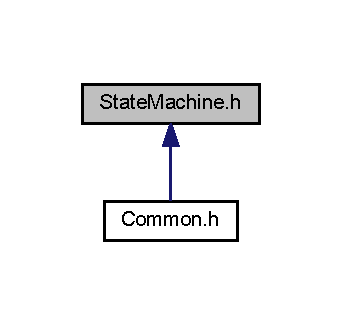
\includegraphics[width=164pt]{_state_machine_8h__dep__incl}
\end{center}
\end{figure}
\subsection*{Functions}
\begin{DoxyCompactItemize}
\item 
void \hyperlink{_state_machine_8h_a8c307b607d4931ec1214de3592c93df4}{sm\-Init} (void)
\end{DoxyCompactItemize}
\subsection*{Variables}
\begin{DoxyCompactItemize}
\item 
void($\ast$ \hyperlink{_state_machine_8h_af1d16f7a57d6ced065765dcbb355fcde}{Alpha\-\_\-\-State\-\_\-\-Ptr} )(void)
\end{DoxyCompactItemize}


\subsection{Detailed Description}
State machine functions. 

\subsection{Function Documentation}
\hypertarget{_state_machine_8h_a8c307b607d4931ec1214de3592c93df4}{\index{State\-Machine.\-h@{State\-Machine.\-h}!sm\-Init@{sm\-Init}}
\index{sm\-Init@{sm\-Init}!StateMachine.h@{State\-Machine.\-h}}
\subsubsection[{sm\-Init}]{\setlength{\rightskip}{0pt plus 5cm}void sm\-Init (
\begin{DoxyParamCaption}
\item[{void}]{}
\end{DoxyParamCaption}
)}}\label{_state_machine_8h_a8c307b607d4931ec1214de3592c93df4}
Sets up the state machine (incl. timers) ready for use. 

\subsection{Variable Documentation}
\hypertarget{_state_machine_8h_af1d16f7a57d6ced065765dcbb355fcde}{\index{State\-Machine.\-h@{State\-Machine.\-h}!Alpha\-\_\-\-State\-\_\-\-Ptr@{Alpha\-\_\-\-State\-\_\-\-Ptr}}
\index{Alpha\-\_\-\-State\-\_\-\-Ptr@{Alpha\-\_\-\-State\-\_\-\-Ptr}!StateMachine.h@{State\-Machine.\-h}}
\subsubsection[{Alpha\-\_\-\-State\-\_\-\-Ptr}]{\setlength{\rightskip}{0pt plus 5cm}void($\ast$ Alpha\-\_\-\-State\-\_\-\-Ptr)(void)}}\label{_state_machine_8h_af1d16f7a57d6ced065765dcbb355fcde}
Runs the next iteration of the state machine. Should be called from the main super-\/loop. 
\hypertarget{_timers_8h}{\section{Timers.\-h File Reference}
\label{_timers_8h}\index{Timers.\-h@{Timers.\-h}}
}


Real and virtual timer functions.  


This graph shows which files directly or indirectly include this file\-:\nopagebreak
\begin{figure}[H]
\begin{center}
\leavevmode
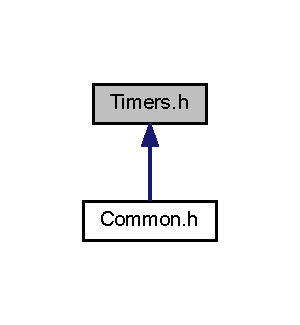
\includegraphics[width=144pt]{_timers_8h__dep__incl}
\end{center}
\end{figure}
\subsection*{Functions}
\begin{DoxyCompactItemize}
\item 
void \hyperlink{_timers_8h_a0a2d06085a127591efdccbedc7b5c4e0}{timers\-Setup\-Virtual} (void)
\item 
void \hyperlink{_timers_8h_a366f5c2927c6a77c9704bee58468a042}{timers\-Setup\-Real} (void)
\end{DoxyCompactItemize}
\subsection*{Variables}
\begin{DoxyCompactItemize}
\item 
int16 \hyperlink{_timers_8h_ade3020803ed700fa7b59b55ca96f2afc}{V\-Timer0} \mbox{[}4\mbox{]}
\item 
int16 \hyperlink{_timers_8h_a2ed6cc170ce3607cf0b5ef1030f11609}{V\-Timer1} \mbox{[}4\mbox{]}
\item 
int16 \hyperlink{_timers_8h_a5e759d74d2b7c1553ba8b2a88122e3a1}{V\-Timer2} \mbox{[}4\mbox{]}
\end{DoxyCompactItemize}


\subsection{Detailed Description}
Real and virtual timer functions. These functions should be run as part of the state machine setup.

\begin{DoxySeeAlso}{See Also}
\hyperlink{_state_machine_8h}{State\-Machine.\-h} 
\end{DoxySeeAlso}


\subsection{Function Documentation}
\hypertarget{_timers_8h_a366f5c2927c6a77c9704bee58468a042}{\index{Timers.\-h@{Timers.\-h}!timers\-Setup\-Real@{timers\-Setup\-Real}}
\index{timers\-Setup\-Real@{timers\-Setup\-Real}!Timers.h@{Timers.\-h}}
\subsubsection[{timers\-Setup\-Real}]{\setlength{\rightskip}{0pt plus 5cm}void timers\-Setup\-Real (
\begin{DoxyParamCaption}
\item[{void}]{}
\end{DoxyParamCaption}
)}}\label{_timers_8h_a366f5c2927c6a77c9704bee58468a042}
Sets up the real timers that run the state machine This should be called as part of the state machine initialisation. \begin{DoxySeeAlso}{See Also}
\hyperlink{_state_machine_8h_a8c307b607d4931ec1214de3592c93df4}{sm\-Init()} 
\end{DoxySeeAlso}
\hypertarget{_timers_8h_a0a2d06085a127591efdccbedc7b5c4e0}{\index{Timers.\-h@{Timers.\-h}!timers\-Setup\-Virtual@{timers\-Setup\-Virtual}}
\index{timers\-Setup\-Virtual@{timers\-Setup\-Virtual}!Timers.h@{Timers.\-h}}
\subsubsection[{timers\-Setup\-Virtual}]{\setlength{\rightskip}{0pt plus 5cm}void timers\-Setup\-Virtual (
\begin{DoxyParamCaption}
\item[{void}]{}
\end{DoxyParamCaption}
)}}\label{_timers_8h_a0a2d06085a127591efdccbedc7b5c4e0}
Sets up the virtual timers for use in the state machine. This should be called as part of the state machine initialisation and before the real timers are setup. \begin{DoxySeeAlso}{See Also}
\hyperlink{_state_machine_8h_a8c307b607d4931ec1214de3592c93df4}{sm\-Init()} 
\end{DoxySeeAlso}


\subsection{Variable Documentation}
\hypertarget{_timers_8h_ade3020803ed700fa7b59b55ca96f2afc}{\index{Timers.\-h@{Timers.\-h}!V\-Timer0@{V\-Timer0}}
\index{V\-Timer0@{V\-Timer0}!Timers.h@{Timers.\-h}}
\subsubsection[{V\-Timer0}]{\setlength{\rightskip}{0pt plus 5cm}int16 V\-Timer0\mbox{[}4\mbox{]}}}\label{_timers_8h_ade3020803ed700fa7b59b55ca96f2afc}
First set of virtual timers. \hypertarget{_timers_8h_a2ed6cc170ce3607cf0b5ef1030f11609}{\index{Timers.\-h@{Timers.\-h}!V\-Timer1@{V\-Timer1}}
\index{V\-Timer1@{V\-Timer1}!Timers.h@{Timers.\-h}}
\subsubsection[{V\-Timer1}]{\setlength{\rightskip}{0pt plus 5cm}int16 V\-Timer1\mbox{[}4\mbox{]}}}\label{_timers_8h_a2ed6cc170ce3607cf0b5ef1030f11609}
Second set of virtual timers. \hypertarget{_timers_8h_a5e759d74d2b7c1553ba8b2a88122e3a1}{\index{Timers.\-h@{Timers.\-h}!V\-Timer2@{V\-Timer2}}
\index{V\-Timer2@{V\-Timer2}!Timers.h@{Timers.\-h}}
\subsubsection[{V\-Timer2}]{\setlength{\rightskip}{0pt plus 5cm}int16 V\-Timer2\mbox{[}4\mbox{]}}}\label{_timers_8h_a5e759d74d2b7c1553ba8b2a88122e3a1}
Third set of virtual timers. 
\hypertarget{_tmp_8h}{\section{Tmp.\-h File Reference}
\label{_tmp_8h}\index{Tmp.\-h@{Tmp.\-h}}
}


Temperature sensor functions.  


This graph shows which files directly or indirectly include this file\-:\nopagebreak
\begin{figure}[H]
\begin{center}
\leavevmode
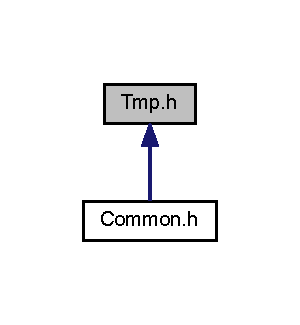
\includegraphics[width=144pt]{_tmp_8h__dep__incl}
\end{center}
\end{figure}
\subsection*{Macros}
\begin{DoxyCompactItemize}
\item 
\#define \hyperlink{_tmp_8h_a5fd3aabe18504a5314a5d0e71e3bc495}{A\-D\-C\-\_\-\-I2\-C\-\_\-\-A\-D\-D\-R}~0x48
\item 
\#define \hyperlink{_tmp_8h_a448e8a52be570dfe9fdddb2045039534}{A\-D\-C\-\_\-\-N\-U\-M\-\_\-\-C\-H\-N\-L}~0x08
\item 
\#define \hyperlink{_tmp_8h_a5a03d0b939a8dda552c9fe3319a82485}{A\-D\-C\-\_\-\-V\-R\-E\-F}~5.\-0
\item 
\#define \hyperlink{_tmp_8h_a9be6401f8c9339711816bec5ca55dd88}{A\-D\-C\-\_\-\-S\-T\-P\-S}~256
\item 
\#define \hyperlink{_tmp_8h_a6d41a70e126c748f2c99c3ff8228eb1b}{T\-M\-P\-\_\-\-V0\-C\-\_\-\-O\-F\-S\-T}~0.\-4
\item 
\#define \hyperlink{_tmp_8h_a0f910bb108922c8686a139977510af53}{T\-M\-P\-\_\-\-S\-C\-L\-\_\-\-O\-F\-S\-T}~\hyperlink{_tmp_8h_a6d41a70e126c748f2c99c3ff8228eb1b}{T\-M\-P\-\_\-\-V0\-C\-\_\-\-O\-F\-S\-T} $\ast$ \hyperlink{_tmp_8h_a9be6401f8c9339711816bec5ca55dd88}{A\-D\-C\-\_\-\-S\-T\-P\-S} / \hyperlink{_tmp_8h_a5a03d0b939a8dda552c9fe3319a82485}{A\-D\-C\-\_\-\-V\-R\-E\-F}
\item 
\#define \hyperlink{_tmp_8h_acc66f9f90ea4746679f5d26c834ddea5}{T\-M\-P\-\_\-\-E\-\_\-\-T\-\_\-\-C\-O\-L\-D}~1.\-5
\end{DoxyCompactItemize}
\subsection*{Functions}
\begin{DoxyCompactItemize}
\item 
Uint16 \hyperlink{_tmp_8h_a4f10186d5fb8a3069cc30c9d0c7e716f}{tmp\-Init} (void)
\item 
Uint16 \hyperlink{_tmp_8h_a10e85d2f2d7cce42822ea65e69601dfa}{tmp\-Set\-Otp} (Uint16 chnl, float32 tmp)
\item 
Uint16 \hyperlink{_tmp_8h_a9aedec904a421fed1823a16846b7841d}{tmp\-Get\-Otp} (Uint16 chnl, float32 $\ast$tmp\-Dest)
\item 
Uint16 \hyperlink{_tmp_8h_adf839085f18308f90ee198a96bbac364}{tmp\-Check\-Otp} (void)
\item 
Uint16 \hyperlink{_tmp_8h_a3f542f4bc433dfd2c1073a5e8308f99f}{tmp\-Read} (Uint16 chnl, float32 $\ast$tmp\-Dest)
\end{DoxyCompactItemize}


\subsection{Detailed Description}
Temperature sensor functions. The temperature sensor (M\-C\-P9701) output is read via an external A\-D\-C (A\-D\-S7830) that is connected to the I2\-C bus at address 10010xx where 'xx' is dependent upon the configuration of resistors R75 -\/ R78. All temperatures are in degrees Celcius.

\begin{DoxyWarning}{Warning}
Before any temperature functions can be used the I2\-C peripheral M\-U\-S\-T be initialised and \hyperlink{_tmp_8h_a4f10186d5fb8a3069cc30c9d0c7e716f}{tmp\-Init()} must be run -\/ \hyperlink{_tmp_8h_a4f10186d5fb8a3069cc30c9d0c7e716f}{tmp\-Init()} will require the interrupts to be enabled globally.
\end{DoxyWarning}
\begin{DoxySeeAlso}{See Also}
\hyperlink{_i2c_8h_a1e0a81a1ad1fd7710ca189236e3e5476}{i2c\-Init()} 
\end{DoxySeeAlso}


\subsection{Macro Definition Documentation}
\hypertarget{_tmp_8h_a5fd3aabe18504a5314a5d0e71e3bc495}{\index{Tmp.\-h@{Tmp.\-h}!A\-D\-C\-\_\-\-I2\-C\-\_\-\-A\-D\-D\-R@{A\-D\-C\-\_\-\-I2\-C\-\_\-\-A\-D\-D\-R}}
\index{A\-D\-C\-\_\-\-I2\-C\-\_\-\-A\-D\-D\-R@{A\-D\-C\-\_\-\-I2\-C\-\_\-\-A\-D\-D\-R}!Tmp.h@{Tmp.\-h}}
\subsubsection[{A\-D\-C\-\_\-\-I2\-C\-\_\-\-A\-D\-D\-R}]{\setlength{\rightskip}{0pt plus 5cm}\#define A\-D\-C\-\_\-\-I2\-C\-\_\-\-A\-D\-D\-R~0x48}}\label{_tmp_8h_a5fd3aabe18504a5314a5d0e71e3bc495}
Slave I2\-C address (A\-D\-S7830 8-\/channel A\-D\-C -\/ A0 = 0, A1 = 0). \hypertarget{_tmp_8h_a448e8a52be570dfe9fdddb2045039534}{\index{Tmp.\-h@{Tmp.\-h}!A\-D\-C\-\_\-\-N\-U\-M\-\_\-\-C\-H\-N\-L@{A\-D\-C\-\_\-\-N\-U\-M\-\_\-\-C\-H\-N\-L}}
\index{A\-D\-C\-\_\-\-N\-U\-M\-\_\-\-C\-H\-N\-L@{A\-D\-C\-\_\-\-N\-U\-M\-\_\-\-C\-H\-N\-L}!Tmp.h@{Tmp.\-h}}
\subsubsection[{A\-D\-C\-\_\-\-N\-U\-M\-\_\-\-C\-H\-N\-L}]{\setlength{\rightskip}{0pt plus 5cm}\#define A\-D\-C\-\_\-\-N\-U\-M\-\_\-\-C\-H\-N\-L~0x08}}\label{_tmp_8h_a448e8a52be570dfe9fdddb2045039534}
Number of temperature channels. The program expects a 50/50 split with first half for the on-\/board temperature channels. \hypertarget{_tmp_8h_a9be6401f8c9339711816bec5ca55dd88}{\index{Tmp.\-h@{Tmp.\-h}!A\-D\-C\-\_\-\-S\-T\-P\-S@{A\-D\-C\-\_\-\-S\-T\-P\-S}}
\index{A\-D\-C\-\_\-\-S\-T\-P\-S@{A\-D\-C\-\_\-\-S\-T\-P\-S}!Tmp.h@{Tmp.\-h}}
\subsubsection[{A\-D\-C\-\_\-\-S\-T\-P\-S}]{\setlength{\rightskip}{0pt plus 5cm}\#define A\-D\-C\-\_\-\-S\-T\-P\-S~256}}\label{_tmp_8h_a9be6401f8c9339711816bec5ca55dd88}
Number of A\-D\-S7830 A\-D\-C steps. \hypertarget{_tmp_8h_a5a03d0b939a8dda552c9fe3319a82485}{\index{Tmp.\-h@{Tmp.\-h}!A\-D\-C\-\_\-\-V\-R\-E\-F@{A\-D\-C\-\_\-\-V\-R\-E\-F}}
\index{A\-D\-C\-\_\-\-V\-R\-E\-F@{A\-D\-C\-\_\-\-V\-R\-E\-F}!Tmp.h@{Tmp.\-h}}
\subsubsection[{A\-D\-C\-\_\-\-V\-R\-E\-F}]{\setlength{\rightskip}{0pt plus 5cm}\#define A\-D\-C\-\_\-\-V\-R\-E\-F~5.\-0}}\label{_tmp_8h_a5a03d0b939a8dda552c9fe3319a82485}
A\-D\-S7830 A\-D\-C reference voltage (volts). \hypertarget{_tmp_8h_acc66f9f90ea4746679f5d26c834ddea5}{\index{Tmp.\-h@{Tmp.\-h}!T\-M\-P\-\_\-\-E\-\_\-\-T\-\_\-\-C\-O\-L\-D@{T\-M\-P\-\_\-\-E\-\_\-\-T\-\_\-\-C\-O\-L\-D}}
\index{T\-M\-P\-\_\-\-E\-\_\-\-T\-\_\-\-C\-O\-L\-D@{T\-M\-P\-\_\-\-E\-\_\-\-T\-\_\-\-C\-O\-L\-D}!Tmp.h@{Tmp.\-h}}
\subsubsection[{T\-M\-P\-\_\-\-E\-\_\-\-T\-\_\-\-C\-O\-L\-D}]{\setlength{\rightskip}{0pt plus 5cm}\#define T\-M\-P\-\_\-\-E\-\_\-\-T\-\_\-\-C\-O\-L\-D~1.\-5}}\label{_tmp_8h_acc66f9f90ea4746679f5d26c834ddea5}
M\-C\-P9701 Error at lowest operating temperature ( $ ^\circ$ C), calculated as shown in Microchip A\-N1001. \hypertarget{_tmp_8h_a0f910bb108922c8686a139977510af53}{\index{Tmp.\-h@{Tmp.\-h}!T\-M\-P\-\_\-\-S\-C\-L\-\_\-\-O\-F\-S\-T@{T\-M\-P\-\_\-\-S\-C\-L\-\_\-\-O\-F\-S\-T}}
\index{T\-M\-P\-\_\-\-S\-C\-L\-\_\-\-O\-F\-S\-T@{T\-M\-P\-\_\-\-S\-C\-L\-\_\-\-O\-F\-S\-T}!Tmp.h@{Tmp.\-h}}
\subsubsection[{T\-M\-P\-\_\-\-S\-C\-L\-\_\-\-O\-F\-S\-T}]{\setlength{\rightskip}{0pt plus 5cm}\#define T\-M\-P\-\_\-\-S\-C\-L\-\_\-\-O\-F\-S\-T~{\bf T\-M\-P\-\_\-\-V0\-C\-\_\-\-O\-F\-S\-T} $\ast$ {\bf A\-D\-C\-\_\-\-S\-T\-P\-S} / {\bf A\-D\-C\-\_\-\-V\-R\-E\-F}}}\label{_tmp_8h_a0f910bb108922c8686a139977510af53}
Scaled temperature offset. \hypertarget{_tmp_8h_a6d41a70e126c748f2c99c3ff8228eb1b}{\index{Tmp.\-h@{Tmp.\-h}!T\-M\-P\-\_\-\-V0\-C\-\_\-\-O\-F\-S\-T@{T\-M\-P\-\_\-\-V0\-C\-\_\-\-O\-F\-S\-T}}
\index{T\-M\-P\-\_\-\-V0\-C\-\_\-\-O\-F\-S\-T@{T\-M\-P\-\_\-\-V0\-C\-\_\-\-O\-F\-S\-T}!Tmp.h@{Tmp.\-h}}
\subsubsection[{T\-M\-P\-\_\-\-V0\-C\-\_\-\-O\-F\-S\-T}]{\setlength{\rightskip}{0pt plus 5cm}\#define T\-M\-P\-\_\-\-V0\-C\-\_\-\-O\-F\-S\-T~0.\-4}}\label{_tmp_8h_a6d41a70e126c748f2c99c3ff8228eb1b}
M\-C\-P9701 Temperature sensor $ V_{0{^\circ}C}$ (volts). 

\subsection{Function Documentation}
\hypertarget{_tmp_8h_adf839085f18308f90ee198a96bbac364}{\index{Tmp.\-h@{Tmp.\-h}!tmp\-Check\-Otp@{tmp\-Check\-Otp}}
\index{tmp\-Check\-Otp@{tmp\-Check\-Otp}!Tmp.h@{Tmp.\-h}}
\subsubsection[{tmp\-Check\-Otp}]{\setlength{\rightskip}{0pt plus 5cm}Uint16 tmp\-Check\-Otp (
\begin{DoxyParamCaption}
\item[{void}]{}
\end{DoxyParamCaption}
)}}\label{_tmp_8h_adf839085f18308f90ee198a96bbac364}
Tests the current on-\/board temperature sensor readings against the O\-T\-P limits. \begin{DoxyReturn}{Returns}
Error status. 
\end{DoxyReturn}
\hypertarget{_tmp_8h_a9aedec904a421fed1823a16846b7841d}{\index{Tmp.\-h@{Tmp.\-h}!tmp\-Get\-Otp@{tmp\-Get\-Otp}}
\index{tmp\-Get\-Otp@{tmp\-Get\-Otp}!Tmp.h@{Tmp.\-h}}
\subsubsection[{tmp\-Get\-Otp}]{\setlength{\rightskip}{0pt plus 5cm}Uint16 tmp\-Get\-Otp (
\begin{DoxyParamCaption}
\item[{Uint16}]{chnl, }
\item[{float32 $\ast$}]{tmp\-Dest}
\end{DoxyParamCaption}
)}}\label{_tmp_8h_a9aedec904a421fed1823a16846b7841d}
Queries the on-\/board over temperature limit for the specified channel. The I2\-C peripheral and temperature reading interface M\-U\-S\-T be initialised before this function is used. 
\begin{DoxyParams}[1]{Parameters}
\mbox{\tt in}  & {\em chnl} & Specifies the channel the setting is to be read from. \\
\hline
\mbox{\tt out}  & {\em tmp\-Dest} & Address of the memory location at which to place the query result ( $ ^\circ$ C). \\
\hline
\end{DoxyParams}
\begin{DoxyReturn}{Returns}
Error status. 
\end{DoxyReturn}
\hypertarget{_tmp_8h_a4f10186d5fb8a3069cc30c9d0c7e716f}{\index{Tmp.\-h@{Tmp.\-h}!tmp\-Init@{tmp\-Init}}
\index{tmp\-Init@{tmp\-Init}!Tmp.h@{Tmp.\-h}}
\subsubsection[{tmp\-Init}]{\setlength{\rightskip}{0pt plus 5cm}Uint16 tmp\-Init (
\begin{DoxyParamCaption}
\item[{void}]{}
\end{DoxyParamCaption}
)}}\label{_tmp_8h_a4f10186d5fb8a3069cc30c9d0c7e716f}
Initialises the system for temperature readings. The I2\-C peripheral must be initialised before this function is used \begin{DoxySeeAlso}{See Also}
\hyperlink{_i2c_8h_a1e0a81a1ad1fd7710ca189236e3e5476}{i2c\-Init()}. 
\end{DoxySeeAlso}
\begin{DoxyReturn}{Returns}
Error status. 
\end{DoxyReturn}
\hypertarget{_tmp_8h_a3f542f4bc433dfd2c1073a5e8308f99f}{\index{Tmp.\-h@{Tmp.\-h}!tmp\-Read@{tmp\-Read}}
\index{tmp\-Read@{tmp\-Read}!Tmp.h@{Tmp.\-h}}
\subsubsection[{tmp\-Read}]{\setlength{\rightskip}{0pt plus 5cm}Uint16 tmp\-Read (
\begin{DoxyParamCaption}
\item[{Uint16}]{chnl, }
\item[{float32 $\ast$}]{tmp\-Dest}
\end{DoxyParamCaption}
)}}\label{_tmp_8h_a3f542f4bc433dfd2c1073a5e8308f99f}
Queries the current on-\/board temperature of the specified channel. 
\begin{DoxyParams}[1]{Parameters}
\mbox{\tt in}  & {\em chnl} & Specifies the channel the temperature is to be read from. \\
\hline
\mbox{\tt out}  & {\em tmp\-Dest} & Address of the memory location at which to place the query result ( $ ^\circ$ C). \\
\hline
\end{DoxyParams}
\begin{DoxyReturn}{Returns}
Error status. 
\end{DoxyReturn}
\hypertarget{_tmp_8h_a10e85d2f2d7cce42822ea65e69601dfa}{\index{Tmp.\-h@{Tmp.\-h}!tmp\-Set\-Otp@{tmp\-Set\-Otp}}
\index{tmp\-Set\-Otp@{tmp\-Set\-Otp}!Tmp.h@{Tmp.\-h}}
\subsubsection[{tmp\-Set\-Otp}]{\setlength{\rightskip}{0pt plus 5cm}Uint16 tmp\-Set\-Otp (
\begin{DoxyParamCaption}
\item[{Uint16}]{chnl, }
\item[{float32}]{tmp}
\end{DoxyParamCaption}
)}}\label{_tmp_8h_a10e85d2f2d7cce42822ea65e69601dfa}
Sets the on-\/board over temperature limit for the specified channel. The I2\-C peripheral and temperature reading interface M\-U\-S\-T be initialised before this function is used. 
\begin{DoxyParams}[1]{Parameters}
\mbox{\tt in}  & {\em chnl} & Specifies the channel the setting is to be applied to. \\
\hline
\mbox{\tt in}  & {\em tmp} & Specifies the value of the limit to be applied ( $ ^\circ$ C). \\
\hline
\end{DoxyParams}
\begin{DoxyReturn}{Returns}
Error status. 
\end{DoxyReturn}

%--- End generated contents ---

% Index
\newpage
\phantomsection
\addcontentsline{toc}{part}{Index}
\printindex

\end{document}
